% Welcome to graphblas-1.0.tex. This is the master LaTex file for the GraphBLAS specification.
%
% The files in this set include:
%
%    ocr-1.0.tex              - this file, the master file
%   ocr.sty                  - the main style file
%   ocr-index.ist            - the index style file
%    titlepage.tex               - the title page
%    ch*.tex                     - the main chapters
%    appendix*.tex               - the appendices
%
% When editing this file:
%
%    1. To change formatting, appearance, or style, please edit ocr.sty.
%
%    2. Custom commands and macros are defined in ocr.sty.
%
%    3. Be kind to other editors -- keep a consistent style by copying-and-pasting to
%       create new content.
%
%    4. We use semantic markup, e.g. (see ocr.sty for a full list):
%         \code{}     % for bold monospace keywords, code, operators, etc.
%         \plc{}      % for italic placeholder names, grammar, etc.
%
%    5. Other recommendations:
%         Use the convenience macros defined in graphblas.sty for the minor headers
%         such as Comments, Syntax, etc.
%
%         To keep items together on the same page, prefer the use of
%         \begin{samepage}.... Avoid \parbox for text blocks as it interrupts line numbering.
%         When possible, avoid \filbreak, \pagebreak, \newpage, \clearpage unless that's
%         what you mean. Use \needspace{} cautiously for troublesome paragraphs.
%
%         Avoid absolute lengths and measures in this file; use relative units when possible.
%         Vertical space can be relative to \baselineskip or ex units. Horizontal space
%         can be relative to \linewidth or em units.
%
%         Prefer \emph{} to italicize terminology, e.g.:
%             This is a \emph{definition}, not a placeholder.
%             This is a \plc{var-name}.
%
%  Acknowlegements: this latex document and style sheet are based on those from the OpenMP 4.0 specification
%

% The following says letter size, but the style sheet may change the size
\documentclass[10pt,letterpaper,twoside,makeidx,hidelinks]{scrreprt}

% Text to appear in the footer on even-numbered pages:
\newcommand{\footerText}{OCR -- Version 1.1.0 -- March 2016}

% Style sheet:
% This is openmp.sty, the preamble and style definitions for the ocr specification.
% This is an include file. Please see the master file for more information.
%
% Quick list of the environments, commands and macros supported. Search below for more details.
%
%    \binding                   % makes header of the same name
%    \comments
%    \constraints
%    \crossreferences
%    \descr
%    \effect
%    \format
%    \restrictions
%    \returns
%    \summary
%    \syntax
%
%    \code{}                    % monospace, bold
%    \plc{}                     % for any kind of placeholder: italic
%    \begin{codepar}            % for blocks of verbatim code: monospace, bold
%    \begin{boxedcode}          % outlined verbatim code for syntax definitions, prototypes, etc.
%    \begin{indentedcodelist}   % used with,e.g., "where clause is one of the following:"
%
%    \specref{}                 % formats the cross-reference "Section X on page Y"
%
%    \notestart                 % black horizontal rule for Notes
%    \noteend
%
%    \cspecificstart            % blue horizontal rule for C-specific text
%    \cspecificend
%
%    \cppspecificstart          % blue horizontal rule for C++ -specific text
%    \cppspecificend
%
%    \ccppspecificstart         % blue horizontal rule for C / C++ -specific text
%    \ccppspecificend
%
%    \fortranspecificstart      % blue horizontal rule for Fortran-specific text
%    \fortranspecificend
%
%    \glossaryterm              % for use in formatting glossary entries
%    \glossarydefstart
%    \glossarydefend
%
%    \compactitem               % single-spaced itemized lists for the Examples doc
%    \cexample                  % C/C++ code example for the Examples doc
%    \fexample                  % Fortran code example for the Examples doc
%
%  Acknowlegement: this style document was borrowed from the OpenMP 4.0 specification
%\include{ocr_doxygen/refman.sty}

\usepackage{comment}            % allow use of \begin{comment}
\usepackage{ifpdf,ifthen}       % allow conditional tests in LaTeX definitions


%%%%%%%%%%%%%%%%%%%%%%%%%%%%%%%%%%%%%%%%%%%%%%%%%%%%%%%%%%%%%%%%%%%%%%%%%%%%%%%%%%%%%%%%%%%%%%
% Document data
%
\author{}


%%%%%%%%%%%%%%%%%%%%%%%%%%%%%%%%%%%%%%%%%%%%%%%%%%%%%%%%%%%%%%%%%%%%%%%%%%%%%%%%%%%%%%%%%%%%%
% Fonts

\usepackage{amsmath}
\usepackage{amsfonts}
\usepackage{amssymb}
\usepackage{courier}
\usepackage{helvet}
\usepackage[utf8]{inputenc}

% Main body serif font:
\usepackage{tgtermes}
\usepackage[T1]{fontenc}


%%%%%%%%%%%%%%%%%%%%%%%%%%%%%%%%%%%%%%%%%%%%%%%%%%%%%%%%%%%%%%%%%%%%%%%%%%%%%%%%%%%%%%%%%%%%%
% Graphic elements

\usepackage{graphicx}
\usepackage{framed}    % for making boxes with \begin{framed}
\usepackage{tikz}      % for flow charts, diagrams, arrows


%%%%%%%%%%%%%%%%%%%%%%%%%%%%%%%%%%%%%%%%%%%%%%%%%%%%%%%%%%%%%%%%%%%%%%%%%%%%%%%%%%%%%%%%%%%%%
% Page formatting

\usepackage[paperwidth=7.5in, paperheight=9in,
            top=0.75in, bottom=1.0in, left=1.4in, right=0.6in]{geometry}

\usepackage{changepage}   % allows left/right-page margin readjustments

\setlength{\oddsidemargin}{0.45in}
\setlength{\evensidemargin}{0.185in}
\raggedbottom


%%%%%%%%%%%%%%%%%%%%%%%%%%%%%%%%%%%%%%%%%%%%%%%%%%%%%%%%%%%%%%%%%%%%%%%%%%%%%%%%%%%%%%%%%%%%%
% Paragraph formatting

\usepackage{setspace}     % allows use of \singlespacing, \onehalfspacing
\usepackage{needspace}    % allows use of \needspace to keep lines together
\usepackage{parskip}      % removes paragraph indenting

\raggedright
\usepackage[raggedrightboxes]{ragged2e}  % is this needed?

\lefthyphenmin=60         % only hyphenate if the left part is >= this many chars
\righthyphenmin=60        % only hyphenate if the right part is >= this many chars


%%%%%%%%%%%%%%%%%%%%%%%%%%%%%%%%%%%%%%%%%%%%%%%%%%%%%%%%%%%%%%%%%%%%%%%%%%%%%%%%%%%%%%%%%%%%%%
% Bulleted (itemized) lists
%    Align bullets with section header
%    Align text left
%    Small bullets
%    \compactitem for single-spaced lists (used in the Examples doc)

\usepackage{enumitem}     % for setting margins on lists
\setlist{leftmargin=*}    % don't indent bullet items
\renewcommand{\labelitemi}{{\normalsize$\bullet$}} % bullet size

% There is a \compactitem defined in package parlist (and perhaps others), however,
% we'll define our own version of compactitem in terms of package enumitem that
% we already use:
\newenvironment{compactitem}
{\begin{itemize}[itemsep=-1.2ex]}
{\end{itemize}}


%%%%%%%%%%%%%%%%%%%%%%%%%%%%%%%%%%%%%%%%%%%%%%%%%%%%%%%%%%%%%%%%%%%%%%%%%%%%%%%%%%%%%%%%%%%%%%
% Tables

% This allows tables to flow across page breaks, headers on each new page, etc.
\usepackage{supertabular}
\usepackage{caption}


%%%%%%%%%%%%%%%%%%%%%%%%%%%%%%%%%%%%%%%%%%%%%%%%%%%%%%%%%%%%%%%%%%%%%%%%%%%%%%%%%%%%%%%%%%%%%
% Line numbering

\usepackage[pagewise]{lineno}       % for line numbers on left side of the page
\pagewiselinenumbers
\setlength\linenumbersep{6em}
\renewcommand\linenumberfont{\normalfont\small\sffamily}
\nolinenumbers            % start with line numbers off


%%%%%%%%%%%%%%%%%%%%%%%%%%%%%%%%%%%%%%%%%%%%%%%%%%%%%%%%%%%%%%%%%%%%%%%%%%%%%%%%%%%%%%%%%%%%%
% Footers

\usepackage{fancyhdr}     % makes right/left footers
\pagestyle{fancy}
\fancyhead{} % clear all header fields
\cfoot{}
\renewcommand{\headrulewidth}{0pt}

% Left side on even pages:
% This requires that \footerText be defined in the master document:
\fancyfoot[LE]{\bfseries \thepage \mdseries \hspace{2em} \footerText}
\fancyhfoffset[E]{4em}

% Right side on odd pages:
\fancyfoot[RO]{\mdseries  \leftmark \hspace{2em} \bfseries \thepage}


%%%%%%%%%%%%%%%%%%%%%%%%%%%%%%%%%%%%%%%%%%%%%%%%%%%%%%%%%%%%%%%%%%%%%%%%%%%%%%%%%%%%%%%%%%%%%
% Section header format - we use four levels: \chapter \section \subsection \subsubsection.

\usepackage{titlesec}     % format headers with \titleformat{}

% Format and spacing for chapter, section, subsection, and subsubsection headers:

\setcounter{secnumdepth}{4}          % show numbers down to subsubsection level

\titleformat{\chapter}[display]%
{\normalfont\sffamily\upshape\Huge\bfseries\fontsize{20}{20}\selectfont}%
{\normalfont\sffamily\scshape\large\bfseries \hspace{-0.7in} \MakeUppercase%
    {\chaptertitlename} \thechapter}%
{0.8in}{}[\vspace{2ex}\hrule]
\titlespacing{\chapter}{0ex}{0em plus 1em minus 1em}{3em plus 1em minus 1em}[10em]

\titleformat{\section}[hang]{\huge\bfseries\sffamily\fontsize{16}{16}\selectfont}{\thesection}{1.0em}{}
\titlespacing{\section}{-5em}{5em plus 1em minus 1em}{1em plus 0.5em minus 0em}[10em]

\titleformat{\subsection}[hang]{\LARGE\bfseries\sffamily\fontsize{14}{14}\selectfont}{\thesubsection}{1.0em}{}
\titlespacing{\subsection}{-5em}{4em plus 1em minus 2.0em}{0.75em plus 0.5em minus 0em}[10em]

\titleformat{\subsubsection}[hang]{\needspace{1\baselineskip}%
\Large\bfseries\sffamily\fontsize{12}{12}\selectfont}{\thesubsubsection}{1.0em}{}
\titlespacing{\subsubsection}{-5em}{3em plus 1em minus 1em}{0.5em plus 0.5em minus 0em}[10em]


%%%%%%%%%%%%%%%%%%%%%%%%%%%%%%%%%%%%%%%%%%%%%%%%%%%%%%%%%%%%%%%%%%%%%%%%%%%%%%%%%%%%%%%%%%%%%%
% Macros for minor headers: Summary, Syntax, Description, etc.
% These headers are defined in terms of \paragraph

\titleformat{\paragraph}[block]{\large\bfseries\sffamily\fontsize{11}{11}\selectfont}{}{}{}
\titlespacing{\paragraph}{0em}{1.5em plus 0.55em minus 0.5em}{0.0em plus 0.55em minus 0.0em}

% Use one of the convenience macros below, or \littleheader{} for an arbitrary header
\newcommand{\littleheader}[1] {\paragraph*{#1}}

\newcommand{\binding} {\littleheader{Binding}}
\newcommand{\comments} {\littleheader{Comments}}
\newcommand{\constraints} {\littleheader{Constraints on Arguments}}
\newcommand{\crossreferences} {\littleheader{Cross References}}
\newcommand{\descr} {\littleheader{Description}}
\newcommand{\effect} {\littleheader{Effect}}
\newcommand{\format} {\littleheader{Format}}
\newcommand{\restrictions} {\littleheader{Restrictions}}
\newcommand{\returns} {\littleheader{Returns}}
\newcommand{\summary} {\littleheader{Summary}}
\newcommand{\syntax} {\littleheader{Syntax}}


%%%%%%%%%%%%%%%%%%%%%%%%%%%%%%%%%%%%%%%%%%%%%%%%%%%%%%%%%%%%%%%%%%%%%%%%%%%%%%%%%%%%%%%%%%%%%%
% Code and placeholder semantic tagging.
%
% When possible, prefer semantic tags instead of typographic tags. The
% following semantics tags are defined here:
%
%     \code{}     % for bold monospace keywords, code, operators, etc.
%     \plc{}      % for italic placeholder names, grammar, etc.
%
% For function prototypes or other code snippets, you can use \code{} as
% the outer wrapper, and use \plc{{} inside. Example:
%
%     \code{\#pragma omp directive ( \plc{some-placeholder-identifier} :}
%
% To format text in italics for emphasis (rather than text as a placeholder),
% use the generic \emph{} command. Example:
%
%     This sentence \emph{emphasizes some non-placeholder words}.

% Enable \alltt{} for formatting blocks of code:
\usepackage{alltt}

% This sets the default \code{} font to tt (monospace) and bold:
\newcommand{\code}[1]{{\texttt{\textbf{#1}}}}
\newcommand{\nspace}[1]{{\textrm{\textmd{ }}}}

% This defines the \plc{} placeholder font to be tt normal slanted:
\newcommand{\plc}[1] {{\textrm{\textmd{\itshape{#1}}}}}

% Environment for a paragraph of literal code, single-spaced, no outline, no indenting:
\newenvironment{codepar}[1]
{\begin{alltt}\bfseries #1}
{\end{alltt}}

% For blocks of code inside a box frame:
\newenvironment{boxedcode}[1]
{\vspace{0.25em plus 5em minus 0.25em}\begin{framed}\begin{minipage}[t]{\textwidth}\begin{alltt}\bfseries #1}
{\end{alltt}\end{minipage}\end{framed}\vspace{0.25em plus 5em minus 0.25em}}

% This sets the margins in the framed box:
\setlength{\FrameSep}{0.6em}

% For indented lists of verbatim code at a relaxed line spacing,
% e.g., for use after "where clause is one of the following:"
\usepackage{setspace}
\newenvironment{indentedcodelist}{%
    \begin{adjustwidth}{0.25in}{}\begin{spacing}{1.5}\begin{alltt}\bfseries}
    {\end{alltt}\end{spacing}\vspace{-0.25\baselineskip}\end{adjustwidth}}


%%%%%%%%%%%%%%%%%%%%%%%%%%%%%%%%%%%%%%%%%%%%%%%%%%%%%%%%%%%%%%%%%%%%%%%%%%%%%%%%%%%%%%%%%%%%%%
% Macros for the black and blue lines and arrows delineating language-specific
% and notes sections. Example:
%
%   \fortranspecificstart
%   This is text that applies to Fortran.
%   \fortranspecificend

% local parameters for use \linewitharrows and \notelinewitharrows:
\newlength{\sbsz}\setlength{\sbsz}{0.05in}  % size of arrows
\newlength{\sblw}\setlength{\sblw}{1.35pt}  % line width (thickness)
\newlength{\sbtw}                           % text width
\newlength{\sblen}                          % total width of horizontal rule
\newlength{\sbht}                           % height of arrows
\newlength{\sbhadj}                         % vertical adjustment for aligning arrows with the line
\newlength{\sbns}\setlength{\sbns}{7\baselineskip}       % arg for \needspace for downward arrows

% \notelinewitharrows is a helper command that makes a black Note marker:
%     arg 1 = 1 or -1 for up or down arrows
%     arg 2 = solid or dashed or loosely dashed, etc.
\newcommand{\notelinewitharrows}[2]{%
    \needspace{0.1\baselineskip}%
    \vbox{\begin{tikzpicture}%
        \setlength{\sblen}{\linewidth}%
        \setlength{\sbht}{#1\sbsz}\setlength{\sbht}{1.4\sbht}%
        \setlength{\sbhadj}{#1\sblw}\setlength{\sbhadj}{0.25\sbhadj}%
        \filldraw (\sblen, 0) -- (\sblen - \sbsz, \sbht) -- (\sblen - 2\sbsz, 0) -- (\sblen, 0);
        \draw[line width=\sblw, #2] (2\sbsz - \sblw, \sbhadj) -- (\sblen - 2\sbsz + \sblw, \sbhadj);
        \filldraw (0, 0) -- (\sbsz, \sbht) -- (0 + 2\sbsz, 0) -- (0, 0);
    \end{tikzpicture}}}

% \linewitharrows is a helper command that makes a blue horizontal line, up or down arrows, and some text:
% arg 1 = 1 or -1 for up or down arrows
% arg 2 = solid or dashed or loosely dashed, etc.
% arg 3 = text
% arg 4 = text width
\newcommand{\linewitharrows}[4]{%
    \needspace{0.1\baselineskip}%
    \vbox to 1\baselineskip {\begin{tikzpicture}%
        \setlength{\sbtw}{#4}%
        \setlength{\sblen}{\linewidth}%
        \setlength{\sbht}{#1\sbsz}\setlength{\sbht}{1.4\sbht}%
        \setlength{\sbhadj}{#1\sblw}\setlength{\sbhadj}{0.25\sbhadj}%
        \filldraw[color=blue!40] (\sblen, 0) -- (\sblen - \sbsz, \sbht) -- (\sblen - 2\sbsz, 0) -- (\sblen, 0);
        \draw[line width=\sblw, color=blue!40, #2] (2\sbsz - \sblw, \sbhadj) -- (0.5\sblen - 0.5\sbtw, \sbhadj);
        \draw[line width=\sblw, color=blue!40, #2] (0.5\sblen + 0.5\sbtw, \sbhadj) -- (\sblen - 2\sbsz + \sblw, \sbhadj);
        \filldraw[color=blue!40] (0, 0) -- (\sbsz, \sbht) -- (0 + 2\sbsz, 0) -- (0, 0);
        \node[color=blue!90] at (0.5\sblen, 0) {\large  \textsf{\textup{#3}}};
    \end{tikzpicture}}}

\newcommand{\VSPb}{\vspace{0.5ex plus 5ex minus 0.25ex}}
\newcommand{\VSPa}{\vspace{0.25ex plus 5ex minus 0.25ex}}

% C
\newcommand{\cspecificstart}{\needspace{\sbns}\linewitharrows{-1}{solid}{C}{3em}}
\newcommand{\cspecificend}{\linewitharrows{1}{solid}{C}{3em}\bigskip}

% C/C++
\newcommand{\ccppspecificstart}{\VSPb\linewitharrows{-1}{solid}{C / C++}{6em}\VSPa}
\newcommand{\ccppspecificend}{\VSPb\linewitharrows{1}{solid}{C / C++}{6em}\VSPa}

% C++
\newcommand{\cppspecificstart}{\needspace{\sbns}\linewitharrows{-1}{solid}{C++}{6em}}
\newcommand{\cppspecificend}{\linewitharrows{1}{solid}{C++}{6em}\bigskip}

% C90
\newcommand{\cNinetyspecificstart}{\needspace{\sbns}\linewitharrows{-1}{solid}{C90}{4em}}
\newcommand{\cNinetyspecificend}{\linewitharrows{1}{solid}{C90}{4em}\bigskip}

% C99
\newcommand{\cNinetyNinespecificstart}{\needspace{\sbns}\linewitharrows{-1}{solid}{C99}{4em}}
\newcommand{\cNinetyNinespecificend}{\linewitharrows{1}{solid}{C99}{4em}\bigskip}

% Fortran
\newcommand{\fortranspecificstart}{\VSPb\linewitharrows{-1}{solid}{Fortran}{6em}\VSPa}
\newcommand{\fortranspecificend}{\VSPb\linewitharrows{1}{solid}{Fortran}{6em}\VSPa}

% Note
\newcommand{\notestart}{\VSPb\notelinewitharrows{-1}{solid}\VSPa}
\newcommand{\noteend}{\VSPb\notelinewitharrows{1}{solid}\VSPa}

% convenience macro for formatting the word "Note:" at the beginning of note blocks:
\newcommand{\noteheader}{{\textrm{\textsf{\textbf\textup\normalsize{{{{Note }}}}}}}}


%%%%%%%%%%%%%%%%%%%%%%%%%%%%%%%%%%%%%%%%%%%%%%%%%%%%%%%%%%%%%%%%%%%%%%%%%%%%%%%%%%%%%%%%%%%%%%
% Glossary formatting

\newcommand{\glossaryterm}[1]{\needspace{1ex}
\begin{adjustwidth}{-0.75in}{0.0in}
\parbox[b][-0.95\baselineskip][t]{1.4in}{\flushright \textbf{#1}}
\end{adjustwidth}}

\newcommand{\glossarydefstart}{
\begin{adjustwidth}{0.79in}{0.0in}}

\newcommand{\glossarydefend}{
\end{adjustwidth}\vspace{-1.5\baselineskip}}


%%%%%%%%%%%%%%%%%%%%%%%%%%%%%%%%%%%%%%%%%%%%%%%%%%%%%%%%%%%%%%%%%%%%%%%%%%%%%%%%%%%%%%%%%%%%%
% Indexing and Table of Contents

\usepackage{makeidx}
\usepackage[nodotinlabels]{titletoc}   % required for its [nodotinlabels] option

% Clickable links in TOC and index:
\usepackage{ifpdf}
\ifpdf
\usepackage[pdftex,pagebackref=true,colorlinks=true,
            linkcolor=blue,unicode,hyperindex=true,linktocpage=true]{hyperref}
\else
\usepackage[ps2pdf,pagebackref=true,colorlinks=true,
            linkcolor=blue,unicode,hyperindex=true,linktocpage=true]{hyperref}
\usepackage{pspicture}
\fi
\hypersetup{
  colorlinks  = true, % Colors links instead of red boxes
  urlcolor    = blue, % Color for external links
  linkcolor   = blue  % Color for internal links
}


%%%%%%%%%%%%%%%%%%%%%%%%%%%%%%%%%%%%%%%%%%%%%%%%%%%%%%%%%%%%%%%%%%%%%%%%%%%%%%%%%%%%%%%%%%%%%
% Formats a cross reference label as "Section X on page Y".

\newcommand{\specref}[1]{Section~\ref{#1} on page~\pageref{#1}}


%%%%%%%%%%%%%%%%%%%%%%%%%%%%%%%%%%%%%%%%%%%%%%%%%%%%%%%%%%%%%%%%%%%%%%%%%%%%%%%%%%%%%%%%%%%%%
% Code example formatting for the Examples document
% This defines:
%     /cexample       formats blue markers, caption, and code for C/C++ examples
%     /fexample       formats blue markers, caption, and code for Fortran examples
% Thanks to Jin, Haoqiang H. for the original definitions of the following:

\usepackage{color,fancyvrb}  % for \VerbatimInput
\usepackage{toolbox}         % for \toolboxMakeSplit

\newcommand{\myreplace}[3]{\bgroup\toolboxMakeSplit*{#1}{DoSplit}%
   \long\def\DoReplace##1{\DoSplit{##1}\lefttext\righttext
   \lefttext
   \toolboxIfElse{\ifx\righttext\undefined}{}%
      {#2\expandafter\DoReplace\expandafter{\righttext}}}%
   \DoReplace{#3}\egroup}

\newcommand{\escstr}[1]{\myreplace{_}{\_}{#1}}

\def\exampleheader#1#2{%
   \ifthenelse{ \equal{#1}{} }{
      \def\cname{#2}
      \def\ename\cname
   }{
      \def\cname{#1.#2}
% Use following line for old numbering
%      \def\ename{\thesection.#2}
% Use following for mneumonics
      \def\ename{\escstr{#1}.#2}
   }
   \noindent
   \textit{Example \ename}
   %\vspace*{-3mm}
}

\def\cnexample#1#2{%
   \exampleheader{#1}{#2}
   %\code{\VerbatimInput[numbers=left,numbersep=14ex,firstnumber=\thelinenumber,firstline=8,fontsize=\small]%
   %\code{\VerbatimInput[numbers=left,firstnumber=1,firstline=8,fontsize=\small]%
   \code{\VerbatimInput[firstline=8,fontsize=\small]%
      {sources/Example_\cname.c}}
}

\def\fnexample#1#2{%
   \exampleheader{#1}{#2}
   %\code{\VerbatimInput[numbers=left,numbersep=14ex,firstnumber=\thelinenumber,firstline=6,fontsize=\small]%
   %\code{\VerbatimInput[numbers=left,firstnumber=1,firstline=8,fontsize=\small]%
   \code{\VerbatimInput[firstline=8,fontsize=\small]%
      {sources/Example_\cname.f}}
}

\newcommand\cexample[2]{%
\needspace{5\baselineskip}\ccppspecificstart
\cnexample{#1}{#2}
\ccppspecificend
}

\newcommand\fexample[2]{%
\needspace{5\baselineskip}\fortranspecificstart
\fnexample{#1}{#2}
\fortranspecificend
}

%% OCR specific macros
\usepackage{listings} % Code snipets

% Some colors we may need
\definecolor{Blue}{rgb}{0.2,0.2,0.8}
\definecolor{Green}{rgb}{0.1,0.5,0.1}
\definecolor{DkBlue}{rgb}{0.1,0.1,0.5}
\definecolor{darkbrown}{rgb}{0.30, 0.30, 0.00}
\definecolor{postit}{rgb}{0.97,1.0,0.54}

% Code environment
\lstdefinelanguage{OCRC}[]{C} {
  morekeywords=[1]{u8, u16, u32, u64, s8, s16, s32, s64, ocrGuid_t,
    ocrEdt_t, ocrEdtDep_t}
}

\lstnewenvironment{ocrsnip}
{
  \lstset{language=OCRC, basicstyle=\scriptsize, breaklines=true,
    breakatwhitespace=true, showstringspaces=false,
    escapeinside={(@}{@)}, numbers=left, numberstyle=\tiny,
    stepnumber=5, numbersep=5pt, frame=single,
    keywordstyle=\bfseries\color{green!40!black},
    commentstyle=\itshape\color{purple!40!black},
    identifierstyle=\color{blue},
    stringstyle=\color{orange}}
}
{
}


%%%%%%%%%%%%%%%%%%%%%%%%%%%%%%%%%%%%%%%%%%%%%%%%%%%%%%%%%%%%%%%%%%%%%%%%%%%%%%%%%%%%%%%%%%%%%
% Support for doxygen generation

\NeedsTeXFormat{LaTeX2e}

\usepackage{array}
\usepackage{calc}
\usepackage{multirow}
\usepackage{longtable}
\usepackage[square,sort,comma,numbers]{natbib}
\usepackage{multicol}
\usepackage{float}
\usepackage{color}
\usepackage{ifthen}
\usepackage{textcomp}
\usepackage{mathptmx}
\usepackage{sectsty}
\usepackage[titles]{tocloft}
\lstset{language=C++,inputencoding=utf8,basicstyle=\footnotesize,breaklines=true,breakatwhitespace=true,tabsize=4,numbers=left }
\hfuzz=15pt
\setlength{\emergencystretch}{15pt}
\hbadness=750
\tolerance=750

\newcommand{\clearemptydoublepage}{%
  \newpage{\pagestyle{empty}\cleardoublepage}%
}
\renewcommand{\chaptermark}[1]{%
  \markboth{#1}{}%
}
\renewcommand{\sectionmark}[1]{%
  \markright{\thesection\ #1}%
}

\newcommand\tabfill[1]{%
  \dimen@\linewidth%
  \advance\dimen@\@totalleftmargin%
  \advance\dimen@-\dimen\@curtab%
  \parbox[t]\dimen@{\raggedright #1\ifhmode\strut\fi}%
}

\newcommand{\ensurespace}[1]{%
  \begingroup
    \setlength{\dimen@}{#1}%
    \vskip\z@\@plus\dimen@
    \penalty -100\vskip\z@\@plus -\dimen@
    \vskip\dimen@
    \penalty 9999%
    \vskip -\dimen@
    \vskip\z@skip % hide the previous |\vskip| from |\addvspace|
  \endgroup
}

% Generic environment used by all paragraph-based environments defined
% below. Note that the command \title{...} needs to be defined inside
% those environments!
\newenvironment{DoxyDesc}[1]{%
  %\ensurespace{4\baselineskip}%
  \begin{list}{}%
  {%
    \settowidth{\labelwidth}{40pt}%
    \setlength{\leftmargin}{\labelwidth}%
    \setlength{\parsep}{0pt}%
    \setlength{\itemsep}{-4pt}%
    \renewcommand{\makelabel}{\entrylabel}%
  }%
  \item[#1]%
}{%
  \end{list}%
}

%---------- Commands used by doxygen LaTeX output generator ----------

% Used by <pre> ... </pre>
\newenvironment{DoxyPre}{%
  \small%
  \begin{alltt}%
}{%
  \end{alltt}%
  \normalsize%
}

% Used by @code ... @endcode
\newenvironment{DoxyCode}{%


\begin{scriptsize}\begin{alltt}%
}{%
\end{alltt}\end{scriptsize}%
}

% Used by @example, @include, @includelineno and @dontinclude
\newenvironment{DoxyCodeInclude}{%
  \DoxyCode%
}{%
  \endDoxyCode%
}

% Used by @verbatim ... @endverbatim
\newenvironment{DoxyVerb}{%
  \footnotesize%
  \verbatim%
}{%
  \endverbatim%
  \normalsize%
}

% Used by @verbinclude
\newenvironment{DoxyVerbInclude}{%
  \DoxyVerb%
}{%
  \endDoxyVerb%
}

% Used by numbered lists (using '-#' or <ol> ... </ol>)
\newenvironment{DoxyEnumerate}{%
  \enumerate%
}{%
  \endenumerate%
}

% Used by bullet lists (using '-', @li, @arg, or <ul> ... </ul>)
\newenvironment{DoxyItemize}{%
  \itemize%
}{%
  \enditemize%
}

% Used by description lists (using <dl> ... </dl>)
\newenvironment{DoxyDescription}{%
  \description%
}{%
  \enddescription%
}

% Used by @image, @dotfile, and @dot ... @enddot
% (only if caption is specified)
\newenvironment{DoxyImage}{%
  \begin{figure}[H]%
  \begin{center}%
}{%
  \end{center}%
  \end{figure}%
}

% Used by @image, @dotfile, @dot ... @enddot, and @msc ... @endmsc
% (only if no caption is specified)
\newenvironment{DoxyImageNoCaption}{%
}{%
}

% Used by @attention
\newenvironment{DoxyAttention}[1]{%
  \begin{DoxyDesc}{#1}%
}{%
  \end{DoxyDesc}%
}

% Used by @author and @authors
\newenvironment{DoxyAuthor}[1]{%
  \begin{DoxyDesc}{#1}%
}{%
  \end{DoxyDesc}%
}

% Used by @date
\newenvironment{DoxyDate}[1]{%
  \begin{DoxyDesc}{#1}%
}{%
  \end{DoxyDesc}%
}

% Used by @invariant
\newenvironment{DoxyInvariant}[1]{%
  \begin{DoxyDesc}{#1}%
}{%
  \end{DoxyDesc}%
}

% Used by @note
\newenvironment{DoxyNote}[1]{%
  \begin{DoxyDesc}{#1}%
}{%
  \end{DoxyDesc}%
}

% Used by @post
\newenvironment{DoxyPostcond}[1]{%
  \begin{DoxyDesc}{#1}%
}{%
  \end{DoxyDesc}%
}

% Used by @pre
\newenvironment{DoxyPrecond}[1]{%
  \begin{DoxyDesc}{#1}%
}{%
  \end{DoxyDesc}%
}

% Used by @copyright
\newenvironment{DoxyCopyright}[1]{%
  \begin{DoxyDesc}{#1}%
}{%
  \end{DoxyDesc}%
}

% Used by @remark
\newenvironment{DoxyRemark}[1]{%
  \begin{DoxyDesc}{#1}%
}{%
  \end{DoxyDesc}%
}

% Used by @return
\newenvironment{DoxyReturn}[1]{%
  \begin{DoxyDesc}{#1}%
}{%
  \end{DoxyDesc}%
}

% Used by @since
\newenvironment{DoxySince}[1]{%
  \begin{DoxyDesc}{#1}%
}{%
  \end{DoxyDesc}%
}

% Used by @see
\newenvironment{DoxySeeAlso}[1]{%
  \begin{DoxyDesc}{#1}%
}{%
  \end{DoxyDesc}%
}

% Used by @version
\newenvironment{DoxyVersion}[1]{%
  \begin{DoxyDesc}{#1}%
}{%
  \end{DoxyDesc}%
}

% Used by @warning
\newenvironment{DoxyWarning}[1]{%
  \begin{DoxyDesc}{#1}%
}{%
  \end{DoxyDesc}%
}

% Used by @internal
\newenvironment{DoxyInternal}[1]{%
  \paragraph*{#1}%
}{%
}

% Used by @par and @paragraph
\newenvironment{DoxyParagraph}[1]{%
  \begin{list}{}%
  {%
    \settowidth{\labelwidth}{40pt}%
    \setlength{\leftmargin}{\labelwidth}%
    \setlength{\parsep}{0pt}%
    \setlength{\itemsep}{-4pt}%
    \renewcommand{\makelabel}{\entrylabel}%
  }%
  \item[#1]%
}{%
  \end{list}%
}

% Used by parameter lists
\newenvironment{DoxyParams}[2][]{%
  \begin{DoxyDesc}{#2}%
    \item[] \hspace{\fill} \vspace{-40pt}%
    \settowidth{\labelwidth}{40pt}%
    \setlength{\LTleft}{0pt}%
    \setlength{\tabcolsep}{0.01\textwidth}%
    \ifthenelse{\equal{#1}{}}%
    {\begin{longtable}{|>{\raggedleft\hspace{0pt}}p{0.15\textwidth}|%
                        p{0.815\textwidth}|}}%
    {\ifthenelse{\equal{#1}{1}}%
      {\begin{longtable}{|>{\centering}p{0.10\textwidth}|%
                         >{\raggedleft\hspace{0pt}}p{0.15\textwidth}|%
                         p{0.685\textwidth}|}}%
      {\begin{longtable}{|>{\centering}p{0.10\textwidth}|%
                         >{\centering\hspace{0pt}}p{0.15\textwidth}|%
                         >{\raggedleft\hspace{0pt}}p{0.15\textwidth}|%
                         p{0.515\textwidth}|}}%
    }\hline%
}{%
    \end{longtable}%
  \end{DoxyDesc}%
}

% Used for fields of simple structs
\newenvironment{DoxyFields}[1]{%
  \begin{DoxyDesc}{#1}%
    \item[] \hspace{\fill} \vspace{-40pt}%
    \settowidth{\labelwidth}{40pt}%
    \setlength{\LTleft}{0pt}%
    \setlength{\tabcolsep}{0.01\textwidth}%
    \begin{longtable}{|>{\raggedleft\hspace{0pt}}p{0.15\textwidth}|%
                         p{0.15\textwidth}|%
                         p{0.635\textwidth}|}%
    \hline%
}{%
    \end{longtable}%
  \end{DoxyDesc}%
}

% is used for parameters within a detailed function description
\newenvironment{DoxyParamCaption}{%
  \renewcommand{\item}[2][]{##1 {\em ##2}}%
  }{%
}

% Used by return value lists
\newenvironment{DoxyRetVals}[1]{%
  \begin{DoxyDesc}{#1}%
    \begin{description}%
      \item[] \hspace{\fill} \vspace{-25pt}%
      \setlength{\tabcolsep}{0.01\textwidth}%
      \begin{longtable}{|>{\raggedleft\hspace{0pt}}p{0.25\textwidth}|%
                          p{0.705\textwidth}|}%
      \hline%
}{%
      \end{longtable}%
    \end{description}%
  \end{DoxyDesc}%
}

% Used by exception lists
\newenvironment{DoxyExceptions}[1]{%
  \begin{DoxyDesc}{#1}%
    \begin{description}%
      \item[] \hspace{\fill} \vspace{-25pt}%
      \definecolor{tableShade}{HTML}{F8F8F8}%
      \rowcolors{1}{white}{tableShade}%
      \arrayrulecolor{gray}%
      \setlength{\tabcolsep}{0.01\textwidth}%
      \begin{longtable}{|>{\raggedleft\hspace{0pt}}p{0.25\textwidth}|%
                          p{0.705\textwidth}|}%
      \hline%
}{%
      \end{longtable}%
    \end{description}%
  \end{DoxyDesc}%
}

% Used by template parameter lists
\newenvironment{DoxyTemplParams}[1]{%
  \begin{DoxyDesc}{#1}%
    \begin{description}%
      \item[] \hspace{\fill} \vspace{-25pt}%
      \definecolor{tableShade}{HTML}{F8F8F8}%
      \rowcolors{1}{white}{tableShade}%
      \arrayrulecolor{gray}%
      \setlength{\tabcolsep}{0.01\textwidth}%
      \begin{longtable}{|>{\raggedleft\hspace{0pt}}p{0.25\textwidth}|%
                          p{0.705\textwidth}|}%
      \hline%
}{%
      \end{longtable}%
    \end{description}%
  \end{DoxyDesc}%
}

\newcommand{\doxyref}[3]{\textbf{#1} (\textnormal{#2}\,\pageref{#3})}
\newenvironment{DoxyCompactList}
{\begin{list}{}{
  \setlength{\leftmargin}{0.5cm}
  \setlength{\itemsep}{0pt}
  \setlength{\parsep}{0pt}
  \setlength{\topsep}{0pt}
  \renewcommand{\makelabel}{\hfill}}}
{\end{list}}
\newenvironment{DoxyCompactItemize}
{
  \begin{itemize}
  \setlength{\itemsep}{-3pt}
  \setlength{\parsep}{0pt}
  \setlength{\topsep}{0pt}
  \setlength{\partopsep}{0pt}
}
{\end{itemize}}
\newcommand{\PBS}[1]{\let\temp=\\#1\let\\=\temp}
\newlength{\tmplength}
\newenvironment{TabularC}[1]
{
\setlength{\tmplength}
     {\linewidth/(#1)-\tabcolsep*2-\arrayrulewidth*(#1+1)/(#1)}
      \par\begin{xtabular*}{\linewidth}
             {*{#1}{|>{\PBS\raggedright\hspace{0pt}}p{\the\tmplength}}|}
}
{\end{xtabular*}\par}
\newcommand{\entrylabel}[1]{
   {\parbox[b]{\labelwidth-4pt}{\makebox[0pt][l]{%
   \usefont{OT1}{phv}{bc}{n}\color{darkgray}#1}\vspace{1.5\baselineskip}}}}
\newenvironment{Desc}
{\begin{list}{}
  {
    \settowidth{\labelwidth}{40pt}
    \setlength{\leftmargin}{\labelwidth}
    \setlength{\parsep}{0pt}
    \setlength{\itemsep}{-4pt}
    \renewcommand{\makelabel}{\entrylabel}
  }
}
{\end{list}}
\newsavebox{\xrefbox}
\newlength{\xreflength}
\newcommand{\xreflabel}[1]{%
  \sbox{\xrefbox}{#1}%
  \setlength{\xreflength}{\wd\xrefbox}%
  \ifthenelse{\xreflength>\labelwidth}{%
    \begin{minipage}{\textwidth}%
      \setlength{\parindent}{0pt}%
      \hangindent=15pt\bfseries #1\vspace{1.2\itemsep}%
    \end{minipage}%
  }{%
   \parbox[b]{\labelwidth}{\makebox[0pt][l]{\textbf{#1}}}%
  }}%
\newenvironment{DoxyRefList}{%
  \begin{list}{}{%
    \setlength{\labelwidth}{10pt}%
    \setlength{\leftmargin}{\labelwidth}%
    \addtolength{\leftmargin}{\labelsep}%
    \renewcommand{\makelabel}{\xreflabel}%
    }%
  }%
{\end{list}}
\newenvironment{DoxyRefDesc}[1]
{\begin{list}{}{%
  \renewcommand\makelabel[1]{\textbf{##1}}
  \settowidth\labelwidth{\makelabel{#1}}
  \setlength\leftmargin{\labelwidth+\labelsep}}}
{\end{list}}
\newenvironment{Indent}
  {\begin{list}{}{\setlength{\leftmargin}{0.5cm}}
      \item[]\ignorespaces}
  {\unskip\end{list}}

\definecolor{comment}{rgb}{0.5,0.0,0.0}
\definecolor{keyword}{rgb}{0.0,0.5,0.0}
\definecolor{keywordtype}{rgb}{0.38,0.25,0.125}
\definecolor{keywordflow}{rgb}{0.88,0.5,0.0}
\definecolor{preprocessor}{rgb}{0.5,0.38,0.125}
\definecolor{stringliteral}{rgb}{0.0,0.125,0.25}
\definecolor{charliteral}{rgb}{0.0,0.5,0.5}
\definecolor{vhdldigit}{rgb}{1.0,0.0,1.0}
\definecolor{vhdlkeyword}{rgb}{0.43,0.0,0.43}
\definecolor{vhdllogic}{rgb}{1.0,0.0,0.0}
\definecolor{vhdlchar}{rgb}{0.0,0.0,0.0}
%%%%%%%%%%%%%%%%%%%%%%%%%%%%%%%%%%%%%%%%%%%%%%%%%%%%%%%%%%%%%%%%%%%%%%%%%%%%%%%%%%%%%%%%%%%%%
% package to support including a PDF file
%\usepackage{pdfpages}
%
%include the whole document             \includepdf[pages=-]{file}
%include a range of pages                 \includepdf[pages2-8]{file}
%include sekecred pages                   \includepdf[pages={3, 6, 1]{file}

% Set default fonts:
\rmfamily\mdseries\upshape\normalsize


% This is the end of openmp.sty of the OpenMP specification.


% Enable the next line to display labels and cross-references for debugging:
%\usepackage{showkeys}

\makeindex

\begin{document}
    \pagenumbering{roman}
    %%%%%%%%%%%%%%%%%%%%%%%%%%%%%%%%%%%%%%%%%%%%%%%%%%%%%%%%%%%%%%%%%%%%%%%%%%%%%%%%%%%%%%%%%%%%%%
% Title page

\begin{titlepage}
%  \begin{flushleft}
%    \hspace{-6em} 
\includegraphics[width=0.4\textwidth]{ocr-logo.png}
%  \end{flushleft}

  \begin{adjustwidth}{-0.75in}{0in}
    \begin{center}
      \Huge
      \textsf{OCR\\The Open Community Runtime \\Interface}

      % An optional subtitle can go here:
      \vspace{0.5in}\textsf{ }\vspace{-0.7in}
      \normalsize
      \vspace{1.0in}
      \textbf{Version 1.2.0 (Candidate Release), December, 2016}
      \vspace{1.0in}

Editors: Tim Mattson, Romain Cledat
    \end{center}
  \end{adjustwidth}
  \vspace{2.0in}

  \begin{adjustwidth}{0pt}{1em}\setlength{\parskip}{0.25\baselineskip}%
Copyright © 2016 OCR working group.\\
Permission to copy without fee all or part of this material is granted,
provided the OCR working group copyright notice and
the title of this document appear.
  \end{adjustwidth}
\end{titlepage}

% Blank page

\clearpage
\thispagestyle{empty}
\phantom{a}
This page intentionally left blank
\vfill


    \setcounter{page}{0}
    \setcounter{tocdepth}{2}

    \begin{spacing}{1.3}
        \tableofcontents
    \end{spacing}

    \chapter*{Acknowledgements}
The OCR specification is an ongoing and collaborative effort in which
multiple people have participated. The following is a partial list of
contributors, in alphebetical order as well as the company or
institution they represented at the time of their contribution:

Jorge Bellon Castro, Intel Corporation and Barcelona Supercomputing Center\\
Zoran Budimlic, Rice University\\
Vincent Cav\'e, Rice University and Intel Corporation\\
Sanjay Chatterjee, Intel Corporation\\
Romain Cl\'edat, Intel Corporation\\
Jiri Dokulil, University of Vienna\\
Roger Golliver, Rice University\\
Min Lee, Intel Corporation\\
Timothy Mattson, Intel Corporation\\
Sri Raj Paul, Rice University\\
Nick Pepperling, Intel Corporation\\
Vivek Sarkar, Rice University\\
Bala Seshasayee, Intel Corporation\\
Rob van der Wijngaart, Intel Corporation\\
Nick Vrvilo, Rice University\\

%    \linenumbers\pagewiselinenumbers
    \newpage\pagenumbering{arabic}

    % This is an included file. See the master file for more information.
%
% This is an included file. See the master file for more information.
%

\chapter{Introduction}
\label{chap:introduction}
Extreme scale computers (such as proposed Exascale computers) contain
so many components that the aggregate mean-time-between-failure (MTBF)
is small
compared to the runtime of an application. Programming models (and
supporting compilers and runtime systems) must therefore support a
variety of features unique to these machines:
\begin{itemize}
\item The ability for a programmer to
express O(billion) concurrency in an application program.

\item The ability of a computation to make progress towards a useful
result even as components within the system fail.

\item The ability of a computation to dynamically adapt to a high
degree of variability in the performance and energy consumption of
system components to support efficient execution.

\item The ability to either hide overheads behind useful computation
or have overheads small enough to allow applications to exhibit strong
scaling across the entire exascale system.

\end{itemize}

There are a number of active research projects to develop runtime systems
for extreme scale computers. This specification describes one of
these research runtime systems: the \emph{Open Community Runtime} or \emph{OCR}.

The fundamental idea behind OCR is to consider a computation as a
dynamically generated directed acyclic graph (DAG) \index{DAG}~\cite{
TaSa11,Tasirlar11,Zuckerman:2011:UCP:2000417.2000424} of tasks
operating on relocatable blocks of data (which we call data blocks in
OCR). Task execution is managed by events.
When the data blocks and events a task depends upon are satisfied, the
preconditions for the execution of the task~\cite{SSWS13} are met and the
task will, at some later point, run on the system. OCR tasks are
\emph{non-blocking}\index{Non-blocking}. This means that once all
preconditions of a task have been met, the task will eventually run to completion
regardless of the behavior of any other tasks or events.

Representing a computation in terms of an event-driven DAG of tasks
decouples the work of a computation
from the ``Units of execution'' that carry out the computation. The work
of a computation is virtualized giving OCR the flexibility to relocate tasks and data
to respond to failures in the system~\cite{Vrvilo14}, achieve a better balance of load
among the processing elements of the computer, or to optimize memory
and energy consumption~\cite{GZCS10,Guo10,CTBCCGYS13,SbBS14}.

Representing the data in terms of data-blocks similarly
decouples the data in a computation from the computer's memory subsystem.
This supports transparent placement and dynamic migration of data
across hardware resources.

OCR is a low level runtime system designed to map onto a wide range of scalable
computer systems.
It provides the capabilities needed to support a wide range of programming models
including data-flow (when events are associated with data blocks),
fork-join (when events enable the execution of post-join
continuations), bulk-synchronous processing (when event trees can be
used to build scalable barriers and collective operations), and
combinations thereof. While some programmers will choose to program directly
at the level of the OCR API, we expect most will use higher level
programming environments that map onto OCR; hence why we describe OCR as a
runtime system rather than an application level programming environment.

\section{Scope}
\label{sec:Scope}

OCR is a vehicle to support research on programming models and
runtime systems for extreme scale
computers~\cite{ExascaleSoftwareStudy2009,SaHS10}. This specification
defines the state of OCR at a fixed point in its development. There
are several limitations in OCR that will be addressed as it continues to
mature.

OCR is a runtime system and collection of low level Application
Programming Interfaces (APIs). While some programmers will directly
work with the APIs defined by OCR, the most common use of OCR will be
to support higher level programming models. Therefore, OCR lacks high
level constructs familiar to traditional parallel programmers such as
\code{reductions} and \code{parallel for}\footnote{Reductions can be
supported in OCR using an accumulator/reducer
approach~\cite{Frigo:2009:ROC:1583991.1584017,SCZS13} and
\code{parallel for} can be supported in OCR
using a fork-join decomposition similar to the cilk\_for construct.}.

All parallelism must be specified explicitly in OCR; OCR does not
extract the concurrency in a program on behalf of a programmer. The
OCR execution model is a low level model; abstract enough to support
relocation of tasks and data to support resiliency or to minimize the
energy consumed by a computation, but low level enough to cleanly map
onto the hardware of extreme scale computers.

OCR is designed to handle dynamic task driven algorithms expressed in
terms of a directed acyclic graph (DAG). In an OCR DAG, each node is
visited only once. This makes irregular problems based on dynamic
graphs easier to express. However, it means that OCR may be less
effective for regular problems that benefit from static load balancing
or for problems that depend on iteration over regular control
structures.
%
% Vivek wanted to put a comment here about the use of annotations to support
% regular algorithms. I opted to not include this since at this time, we don't have
% such annotations in OCR. When we add them and show that the address this problem,
% we can update this text accordingly.

OCR is defined in terms of a C library. Programs written in any
language that includes an interface to C should be able to work with
OCR.

OCR tasks are expressed as event driven tasks (EDTs).
The overheads associated with OCR API calls depend on the underlying
system software and hardware. On current systems, the overhead of
creating and scheduling an event driven task can be fairly high.
On system with hardware support for task queues, the
overheads can be significantly lower. An OCR programmer should experiment with their
implementation of OCR to understand the overheads associated with managing EDTs and
assure that the work per EDT is great enough to offset OCR overheads.

OCR is currently a research runtime system, developed as an
open-source community project. It does not as yet have the level of
investment needed to develop a production system that can be used for
serious application deployment.
% This is the end of ch1-intro.tex of the OCR specification.
%
% This is an included file. See the master file for more information.
%

%
\section{Glossary}
\label{sec:Glossary}
\glossaryterm{Acquired}
\index{Acquired}
\glossarydefstart
The state of a data block when its chunk of data is accessible to an
OCR object. For example, an EDT must acquire a data block before it
can read-from or write-to that data block.
\glossarydefend

\glossaryterm{Data Block (DB)}
\index{Data Block}
\glossarydefstart
The data, used by an OCR object such as an EDT, that is intended for
access by other OCR objects. A data block specifies
a chunk of data that is entirely accessible as an offset from a starting address.
\glossarydefend

\glossaryterm{Dependence}
\index{Dependence}
\glossarydefstart
A dependence is a link between the post-slot of a source event or
data-block and the pre-slot of a destination EDT or event. The
satisfaction of the source OCR object's post-slot will trigger the
satisfaction of the destination OCR object's pre-slot.
\glossarydefend

\glossaryterm{Event driven Task (EDT)}
\index{Event Driven Task}\index{EDT}
\glossarydefstart
An OCR object that implements the concept of a task. An EDT with $N$
dependences will have $N$ \emph{pre-slots} numbered from $0$ to $N-1$
and one post-slot.
Each of the \emph{pre-slots} associated with an EDT connects to a
single OCR object, while the EDT’s single \emph{post-slot} can connect
to multiple OCR objects. An EDT transitions to the \emph{ready} state when all its
pre-slots have been satisfied; the pre-slots determine which
data blocks, if any, the EDT may access.  Once an EDT is in the ready state, it will 
eventually run on the OCR platform.
\glossarydefend

% Vivek writes ...
%An EDT may have zero or more pre-slots that serve as preconditions. Each pre-slot is associated with a
% single OCR event. An EDT also has a single post-slot that is associated with the event that represents
%the completion of the EDT's execution.
%
%NOTE: I really like the text below on how the DAG is defined, but I'm not sure that it belongs in
%the glossary. It might be better to create a separate section titled something like "Computation DAG"
%and use that to explicitly define the DAG referred to in Section 1.1. That new subsection should include
%figures, with a graphical notation (e.g.,with input ports for each of the pre-slots) that makes the points
% in the text very clear. I'd be happy to provide text for that  subsection, if needed.
%
% TGM responds ... I like much of what Vivek is saying here, but we don't have time to update the
%definition as he suggested (we'd need to define a continuation for example). We may choose to
% add that section, but we'll have to also discuss that for a later day. The problem is that every
% presentation I've seen that uses the graphical representation vivek alludes to makes things
% less clear, not more clear. This is the same problem I have with CnC which is only clear
% and easy to understand by the handful or people who created it or worked directly with it. To
% an application programmer, their diagrams are just a confusing mess. The same holds for OCR
% so we need to figure out how to fix this before we work it into the spec.
\glossaryterm{EDT function}
\index{EDT function}
\glossarydefstart
The function that defines the code to be executed by an EDT. The function
takes as arguments the number of parameters, the actual array of
parameters, the number of dependences and the actual array of
dependences. \emph{Parameters} are static 64-bit values known at EDT
creation time and \emph{dependences} are dynamic control or data
dependences. The parameter array is copied by value when the EDT is
created and enters the \emph{available} state. The dependences (namely the array of dependences) are
determined at runtime and are fully resolved only when the EDT is launched and 
is ready to execute. The EDT function can optionally return the GUID of a Data Block or
event that will be passed along its ``post'' slot.

\glossarydefend
\glossaryterm{EDT template}
\index{EDT template}
\glossarydefstart
An OCR object from which an EDT instance is created. The EDT template
stores meta-data related to the EDT definition, the EDT function, and
the number of parameters and dependences available to EDTs
instantiated (created) from this template. Multiple EDTs can be created from the
same EDT template.
\glossarydefend


%%
%TGM:  Rob urges us to put all the event definitions together. We may want to organize this glossary along the lines
% of what is done in the OpenMP specification .... a high level topical break-down and alphabetical inside
% at topic.

\glossaryterm{Event}
\index{Event}
\glossarydefstart
An OCR object used as an indirection mechanism between other OCR
objects interested in each other's change of state (unsatisfied to
satisfied). Events are the main synchronization mechanism in OCR.
\glossarydefend

\glossaryterm{Finish EDT}
\index{Finish EDT}
\glossarydefstart
A special class of EDT. As an EDT runs, it may create additional EDTs
which may themselves create even more EDTs. 
For the case of a finish
EDT, the EDTs created within its scope (i.e.\ its child EDTs and further
descendants) complete and satisfy their post-slots
before the finish EDT can satisfy its post-slot. The result is that
any OCR object linked to the post-slot of the finish EDT will by
necessity not be enter the \emph{ready} state (i.e. be scheduled for 
execution) until the finish EDT and all
EDTs created during its execution have completed.
%
% The following text from Vivek is more precise, but it generates a latex error when I 
% try to typeset it.  
%
%For the case of a Finish EDT, F, each EDT created with F identified 
%as its Immediately Enclosing Finish (IEF) 
%must complete execution and satisfy its post-slot before Finish EDT F can satisfy its post-slot.
%The result is that any OCR object linked to the post-slot of 
%the finish~EDT will by necessity
%wait until finish~EDT F and all EDTs that have F as their IEF have completed.

\glossarydefend


\glossaryterm{Globally Unique ID (GUID)}
\index{Globally Unique ID}\index{GUID}
\glossarydefstart
A value generated by the runtime system that uniquely identifies each
OCR object. The GUIDs for the OCR objects reside in a global name
space visible to all EDTs.
\glossarydefend

% Vivek writes ...
%
%  A 64-bit value that uniquely identifies each OCR object. The GUIDs for the OCR
% objects reside in a global name space visible to all EDTs. Creation and management
% of GUIDs is managed by the OCR runtime by default, though user input can also be
% used to influence GUID allocation, if so desired.
%
% TGM responds ... two problem. Why does it have to be 64 bit as defined in the spec?   I don't
% get that. Second, the current API doesn't provice uer input to influce GUID allocation so
% we can't say this yet. Right?

\glossaryterm{Latch Event}
\index{Latch Event}
\glossarydefstart
A special type of event that propagates a satisfy signal to its post-slot
when it has been satisfied an equal number of times on each of its two
pre-slots. In other words, if you imagine a
monotonically increasing counter on each of the two pre-slots, the
latch event's post-slot will be satisfied if and only if both monotonically
increasing counters are non-zero and equal. Note that once the latch
event's post-slot is satisfied, satisfaction on the latch event's
pre-slots will result in undefined behavior; the latch event will
therefore only satisfy its post-slot at most one time.
\glossarydefend

% vivek writes ...
%(See earlier note re. definition of pre-slots and post-slots for events.)
%
%Need to clarify that the post-slot of the latch event can only be triggered once.
%
%Also, a problematic aspect of a latch event is that it appears that a pre-slot can
%be "triggered" multiple times. Maybe it should not be called a pre-slot?
%
%In general, it feels like we need an OO-style abstraction for events, in which an
%event has a void satisfy function with a parameter list that includes the pointer to
%the satisfy function, and an argc, argc pair that represents arguments for the function.
% One challenge is where to store the internal state of the event. Seems like it needs
% to be in a data block?

%TGM responds ... this is another case where I didnt' want to make major changes to
% this without a long discussion with the group. I can't tell you how much time we  spent
%creating the current definition so changes would be problematic.
%
% I wanted to capture Vivek's comments espeically about the OO suggestion. I think he
% is touching on something very important there and we need to dsicuss this in more
% detail.
%
% REC: I agree with his OO-style of abstraction. I have always (but
% probably not very clearly) tried to say that events have a mini
% ``rule'' that determines when its post-slot get satisfied. As for
% the state to store, it's in the metadata

\glossaryterm{OCR object}
\index{OCR object}
\glossarydefstart
A reference counted object managed by OCR. \emph{EDTs}, \emph{events},
\emph{templates}, and \emph{data blocks} are the most frequently
encountered examples of OCR objects. Each OCR object has a unique
identifier, or GUID.
\glossarydefend

\glossaryterm{OCR program}
\index{OCR program}
\glossarydefstart
A program that is conformant to the OCR specification. Statements in
the OCR specification about the OCR program only refer to behaviors
associated with the constructs that make up OCR. For example, if an
OCR program were to use a parallel programming model outside of OCR,
that program is no longer a purely conformant OCR program and its
behavior can no longer be defined by OCR.
\glossarydefend

\glossaryterm{Released}
\index{Released}
\glossarydefstart
The state of a data block that is no longer accessible by a certain OCR
object. For example, after an EDT has finished all of its
modification to a data block and it is ready to make those
modifications accessible by other EDTs, it must release that data
block.
\glossarydefend

\glossaryterm{Slot}
\index{Slot}
\glossarydefstart
Positional end point for a dependence. An OCR object has one or more
slots. Exactly one slot is a \emph{post-slot}. This is used to
communicate the state of the OCR object to other OCR objects. The
other zero of more slots are \emph{pre-slots}, which are used to manage
input dependences of the OCR object. A slot can be:
\begin{itemize}
\item Unconnected: There are no links connecting to the slot;
\item Connected: a link attaches a source post-slot to a destination pre-slot.
\end{itemize}
A slot in the \emph{connected} state can be:
\begin{itemize}
\item Satisfied: the source of the link has been triggered;
%\item Triggered: see 'Trigger';
\item Unsatisfied: the source of the link has not been triggered.
\end{itemize}
\glossarydefend

\glossaryterm{Task}
\index{Task}
\glossarydefstart
A non-blocking set of instructions that constitute the fundamental
``unit of work'' in OCR.  By ``non-blocking'' we mean that once all
preconditions on a task are met, the task is ``ready to execute'' 
and it will execute at some point,
regardless of what any other task in the system does. The concept of
a task is realized by the OCR object ``Event Driven Task'' or EDT.
\glossarydefend

\glossaryterm{Trigger}
\index{Trigger}
\glossarydefstart
This term is used to describe the action of either a ``satisfied''
post-slot or of an event whose trigger rule is satisfied. In the
former case, when a post slot on
an OCR object is satisfied, it triggers any connected
pre-slots causing them to become ``satisfied''. In the latter case,
when an event's trigger rule is satisfied (due to satisfaction(s) on its
pre-slot(s)), it satisfies its post-slot. Therefore, for most events,
when the event's pre-slot becomes satisfied, this will trigger the event and
therefore cause it to satisfy its post-slot which will in turn trigger
the dependence link and satisfy all pre-slots connected to the event's
post-slot. The conjugated form \emph{triggered} is used as an
attributive past participle; that is
``an EDT that has finished executing the code in its EDT function and  
released its data blocks will satisfy the event associated
with its post-slot and become a triggered EDT''.
\glossarydefend


\glossaryterm{Unit of Execution}
\index{Unit of Execution}\index{UE}
\glossarydefstart
A generic term for a process, thread, or any other executable agent
that carries out the work associated with a program.
\glossarydefend

% vivek wants us to consider and more carefully define the idea of the wrok assocaited with a
% computation. See his feedback on the version 1.0 spec for details.


\glossaryterm{Worker}
\index{Worker}
\glossarydefstart
The unit of execution (e.g.\ a process or a thread) that carries out
the sequence of instructions associated with the EDTs in an OCR
program. The details of a worker are tied to a particular
implementation of an OCR platform and are not defined by OCR.
\glossarydefend

% This is the end of ch1-glossary of the OCR specification.
% This is an included file. See the master file for more information.
%

\section{The core elements of OCR}
\label{sec:OCRElements}

clearn this up.  Make sure it clearly states that tasks have transactional semantics
in order to support resiliancy models.

An OCR program\index{OCR program} is best understood as a dynamically created,
directed acyclic graph
(DAG)\index{DAG}~\cite{TaSa11,Tasirlar11,Zuckerman:2011:UCP:2000417.2000424}.
The vertices in the graph are OCR objects that define a computation:
tasks\index{Task} which perform the actual computation and
events\index{Event} which are used to coordinate the
activity of other objects. The edges are dependences between objects
(i.e.\ a \emph{link}) which can represent data dependences (events with
an associated data block) or pure control dependences (events).

The tasks within the DAG represent the work carried out by an OCR
program. Edges impinging on a task define preconditions for the execution of
the task~\cite{SSWS13}. Tasks whose preconditions have been met are
\emph{runnable}\index{Runnable}. Outgoing edges define dependences and
triggers for later objects in the graph. OCR tasks are
\emph{non-blocking}\index{non-blocking}. This means that once all
preconditions on a task have been met, the task becomes runnable, and
when it begins to execute; the task will eventually run to completion
regardless of the behavior of any other OCR objects.

OCR programs can either run alone or be encompassed in other programs
in a library manner. In the following description, ``OCR program'' refers
to either the entire OCR program if it is running alone or the OCR
portion of the program if running library mode.

The OCR program logically starts as a single task, dynamically builds the
DAG corresponding to the executing program, and completes when the
\code{ocrShutdown()} or \code{ocrAbort()} function is called.
This rather simple model can handle a wide range of
design patterns including branch and bound, data flow, and divide and
conquer.
%
%Vivek wanted to add a long discusssion of how you can use to represent
% SPMD algorithms as well. Once again, given the short time to address this,
% I opted to leave it out. This is a specfication not a programmers reference guide. But
% he rasied many good points that we need to develop and docuent somewhere
%
With both data and tasks conceptually decoupled from their realization
on a computer system, OCR has the flexibility to relocate tasks and data
to respond to failures in the system, achieve a better balance of load
among the processing elements of the computer, or to optimize memory
and energy consumption~\cite{GZCS10,Guo10,CTBCCGYS13,SbBS14}.

We will define the execution model in OCR by starting with a model of
the OCR platform. We will then describe the fundamental objects used
to define OCR. Finally, we will describe the details of how an OCR
program executes.


\subsection{OCR objects}
\index{OCR object}
\label{sec:OCRobjects}

An OCR object is a reference counted entity managed by OCR. Every OCR
object has a globally unique ID (GUID) that is used to identify the
object. Objects have two well defined states.
\begin{enumerate}
\item \emph{Created}: Resources associated with an object and its GUID
have been created.
\item \emph{Destroyed}: An object that is destroyed is marked for
destruction when the destruction command executes. A destroyed object
and any resources associated with the destroyed object are no longer
defined. The object is not actually destroyed and the associated
resources are not freed until the reference count is zero\footnote{As
an optimization, the runtime may choose to reuse of the same physical
object for different logical objects~\cite{USBCSS12,SbKS12}.}.
%
%  Vivek suggest we call this "Dead" instead of "destroyed".  He provided new text in his feedback to
% address this. I wouild have put his text here, but I can't cut and paste from his document. But
% if we all agree, we should look at his feedback document and add this later.
\end{enumerate}
Furthermore, for OCR data blocks, we have two additional states:
\begin{enumerate}
\item \emph{Acquired}: the data associated with the data block has
become accessible to the acquiring OCR object thereby incrementing the
acquired objects reference count.
\item \emph{Released}: The object is no longer accessible by the OCR
object that had earlier acquired it. The reference count on the
released object is decremented.
\end{enumerate}

An OCR program is defined in terms of three fundamental objects.
\begin{itemize}
\item \emph{Event Driven Tasks (EDT)} A non-blocking unit of work in an OCR
program.
\item\emph{Data blocks (DB)}A contiguous block of memory managed by the
OCR runtime accessible to any OCR objects to which it is linked.
\item\emph{Events} An object to manage dependences between OCR objects and
to define ordering relationships (synchronization) between them.
\end{itemize}

In addition to these fundamental objects, OCR defines a number of
associated objects that simplify OCR programming or support specific
desired behaviors of the fundamental objects.
%\begin{description}
\begin{itemize}
\item \emph{EDT Template} An OCR object used to manage the resources
required to create an EDT.
\item \emph{Affinity container} An OCR object used to influence the
placement of EDTs in an executing program.
\end{itemize}


\subsection{OCR Platform}
\index{OCR Platform}
\label{sec:OCRPlatform}

An OCR program executes on an abstract machine called the \emph{OCR
Platform}.  The OCR platform is a resource that can carry out
computations. It consists of:
\begin{itemize}
\item A collection of network connected nodes where any two nodes can
communicate with each other.
\item Each node consists of one or more processing elements each of
which has its own private memory\footnote{By ``private'' we mean a
memory region that is not accessible to other processing
elements.}.
\item A globally accessible shared namespace of OCR objects each
denoted by a globally unique ID (GUID).
\end{itemize}
OCR is designed to be portable and scalable, hence, the OCR Platform
places minimal constraints on the physical hardware.

As dependences are met for the tasks in an OCR program's DAG, the
tasks become \emph{runnable}. These tasks and any resources required
to support their execution are then submitted to
\emph{workers}\index{Worker}~\cite{GBRS09} which execute the tasks on
the processing elements within the OCR platform. The workers and the
data-structures used to store tasks waiting to execute
(i.e.\ work-pools) are a low level implementation detail not defined by
the OCR specification. When reasoning about locality and load
balancing, programmers may need to explicitly reason about the
behavior of the workers~\cite{Chatterjee13}, but they do not hold
persistent state visible to an OCR program and are logically opaque to
OCR constructs.
%
% vivek added ...
%Tuning annotations for locality can be specified in OCR in the form of preferred affinities (co-location)
% among EDTs and/or data blocks.
%
% TGM responds ... I didn't see this anywhere in the current API. Did I miss something?  If they aren't there
% we can't put them in the spec. If they are there, we need to talk about this and figure out how
% to add this to the spec.
% REC: They are still being defined and are not solidly fixed
% yet. Zoran, Sanjay and Rob are discussing them.

\subsection{Dependences, Links and slots}
\index{OCR links}
\label{sec:OCRlinks}


An OCR program defines a graph with the three fundamental OCR objects
(EDTs, DBs and Events) as the nodes of the graphs and edges are
\emph{links}\index{Link} between objects. A link defines a dependence
between OCR objects. The links are defined in terms of
\emph{slots}\index{Slot} on the OCR object. A slot defines an end
point for a dependence for an OCR object.

Event, data blocks and EDTs each have a single \emph{post
slot}\index{post-slot}.  used to communicate the state of an OCR
object to other OCR objects. For example, if an EDT wanted to let
another EDT know that it had finished its assigned work, it could do
so by signaling over its post-slot that it is \emph{satisfied} or
equivalently, that the post-slot is \emph{triggered}. The rules
defining when a post slot triggers, the so-called \emph{post-slot
trigger rule}\index{post-slot trigger rule} depends on the type of OCR
object and is discussed in Section~\ref{sec:triggerrule}.

Some OCR objects (such as EDTs) can also have an optional set of
\emph{pre-slots}\index{pre-slot}. A pre-slot defines an incoming
dependence or a pre-condition for execution by an EDT. The post-slot
of one EDT, for example, can be connected to the pre-slot of another
EDT thereby establishing a control dependence\index{control
dependence} between the EDTs. Likewise,
the post-slot of a data block can be connected to the pre-slot of an EDT
to establish an immediately satsified data dependence.

Slots are used along with data block objects to define data
dependences\index{data dependence} between OCR objects. For example,
for producer consumer relationships\index{producer consumer
relationships} the post slot of the producer EDT can be connected to
the pre-slot of the consumer EDT. When the producer finishes its work
and updates the data block it wishes to share, it associates that data
block with the post-slot and signals its ``satisfied'' state to the
consumer who can then safely begin working with the data block from
the producer.

Refer to Section~\ref{sec:Glossary} for a definition of the states of
a Slot. All slots are initially in the \code{unconnected} state. Data
block post slots are immediately \code{satisfied} as soon as they are
connected.

\subsection{EDTs}
\index{EDT}
\label{sec:EDT}

A task defines the basic unit of work within a programming model. As
mentioned earlier, a task is a non-blocking unit of work. Once all
pre-conditions on the OCR task have been met, it becomes
runnable\index{Runnable} or ``available to execute'' and once it
begins execution it executes without waiting on any other OCR
objects. In OCR, we package a task into an Event Driven
Task\index{Event Driven Task} or an EDT\index{EDT}.

The EDT is created as an instance of an \emph{EDT template}\index{EDT
template}. This template stores metadata about EDTs created from the
template, optionally defines the number of dependences and parameters
used when creating an instance of an EDT, and is a container for the
function that will be executed by an EDT. This function is called the
\emph{EDT function}\index{EDT function}.

The OCR API defines the function prototype and return values expected
by an EDT function. These include:
\begin{itemize}
\item The parameters of the EDT function which are copied by value
when the EDT is created.
\item Dynamic dependences expressed through a dependence array that is
formed at runtime from explicit user-specified dependences.
\item An optional GUID of a OCR object holding data (a \emph{data
block}) that will be used to satisfy the EDT’s post slot. This is the
return value of the function.
\end{itemize}
When \code{ocrEdtCreate()} is used to create an EDT, it returns one or
two GUIDs: the first (always returned) is the GUID for the EDT itself;
the second (returned only on programmer request) is the GUID of the
event implied by the post slot of the EDT\footnote{It is important to
  note that although, semantically, an EDT can be the source of a
  dependence, when adding a dependence, the programmer must use the
  GUID of the associated event as the source.}
When the OCR function returns a data block, the GUID of
that data block is used to satisfy the implied event.

Using a post-slot in a link to another object is just one method to
trigger other OCR objects. OCR includes the \code{ocrEventSatisfy()}
API to trigger other OCR objects through explicitly created dependence
links.

OCR defines one special type of EDT; the \emph{finish
EDT}\index{Finish EDT}. An EDT always executes asynchronously and
without blocking once all of its pre-conditions have been met. A
finish EDT, however, will not trigger its post-slot until all EDTs
launched within its scope (i.e.\ its child EDTs and EDTs created
within its child EDTs) have completed.  The finish EDT still executes
asynchronously and without blocking. The implied event associated with
the post slot of a finish EDT is a \emph{latch event}, i.e.\ it is
connected to the post-slots of all EDTs created within its scope and
does not trigger until they have all finished.

\subsection{Events}
\index{Event}
\label{sec:Event}

An event is an OCR object used to coordinate the activity of other OCR
objects. As with any OCR object, events have a single
post-slot. Events may also have one or more pre-slots; the actual
number of which is determined by the type of event.

The post-slot of an event can be connected to multiple OCR objects by
connecting the single post-slot to the pre-slots of other OCR objects.
When the conditions are met indicating that the event should trigger
(according to the \emph{trigger rule}\index{trigger rule}), the event
sets its post-slot to \emph{satisfied} therefore establishing an
ordering relationship between the event and the OCR objects linked to
the event. Events therefore play a key role in establishing the
patterns of synchronization required by a parallel
algorithm~\cite{ImSa14-2}.

When an event is satisfied, it can optionally attach a data block to
the post slot. Hence, events not only provide synchronization
(control dependences) but they are also the mechanism OCR uses to
establish data flow dependences. In other words, a classic data flow
algorithm defines tasks as waiting until data is ``ready''. In OCR
this concept is implemented through events with attached data blocks.

Given the diversity of parallel algorithms, OCR has defined several
types of events:
\begin{enumerate}
\item \emph{Once event}\index{Event, Once}: The event is automatically
destroyed on satisfaction. Any object that has the Once event as a
pre-condition must already have been created and linked by the time
the Once event is satisfied.

\item \emph{Idempotent event}\index{Event, Idempotent}: The event
exists until explicitly destroyed by a call to
\code{ocrEventDestroy()}. It is satisfied once and subsequent attempts
to satisfy (i.e.\ trigger) the event are ignored.

\item \emph{Sticky event}\index{Event, Sticky}: The event exists until
explicitly destroyed with a call to \code{ocrEventDestroy()}. It is
satisfied once and subsequent attempts to satisfy (i.e.\ trigger) the
event result in an error code being returned when trying to satisfy
the event.
%
%  Vivek writes:  Need to state the meaning of an error in OCR. Does it result in program
% termination, or some sort of error code (since there is no support for exceptions in C),
% or is it simply undefined?
%
%  TGM respondes ... yes, I am in violent agreement with Vivek. I just don't know
% how to do this right now in fits in with the overall design of OCR. This shojld be
% a major discussion point following the apps workshop
% REC: I added a small note saying it is an error code
%
\item \emph{Latch event}\index{Event, Latch}: The latch event has two
pre-slots and triggers when the conditions defined by the latch
trigger rule are met. The event is automatically destroyed once it
triggers; in this regard, it is similar to a \emph{once event}.
\end{enumerate}
Events have one pre-slot except for latch-events which have two pre-slots.

\subsubsection{Trigger rule}
\label{sec:triggerrule}
Events ``trigger'' when the appropriate \emph{trigger
rule}\index{trigger rule} is met. The default trigger rule for events
is when the link on their pre-slot is satisfied, the event triggers
and passes the state from the pre-slot to its post slot. For example,
if the pre-slot has an associated data block GUID, that data block
GUID will be propagated through the event's post slot.

The trigger rule for a latch event is somewhat more complicated. The
latch event has two pre-slots; an increment slot and a decrement
slot. The latch event will trigger its post-slot when the event
receives an equal but non-zero number of satisfy notifications on each
of the pre-slots. Once a latch event triggers, any subsequent
triggers on the pre-slots of the latch event are undefined. For
regular events, when it is triggered with a data block, the GUID of
that data block is passed along through the post-slot of the
event. For a latch event, however, the GUID of a data block that
triggers a pre-slot is ignored.

\subsection{Data Blocks}
\index{Data Block}
\label{sec:datablocks}
Data blocks are OCR objects used to hold data in an OCR program. A
data block is the only way to store data that persists outside of the
scope of a collection of EDTs. Hence, data blocks are the only way to
share data between EDTs. The data blocks are identified by their
GUIDs and occupy a shared name space of GUIDs. While the name space
is shared and globally visible, however, an EDT can only access {\bf a)}
data blocks passed into the EDT through a pre-slot or {\bf b)} a data block
that is created inside the body of the EDT.

When a data block is created, the default behavior is that the EDT
that created the data block will also acquire the data block. This
increments the reference counter for the data block and plays a key
role in managing the memory of an OCR program. Optionally, an EDT can
create a data block on behalf of another EDT. In this case, a
programmer can request that the data block is created, but not
acquired by the EDT.

Conceptually, data blocks are contiguous chunks of memory
that have a start address and a size. They have the following characteristics:
\begin{itemize}
\item all memory within the data block is accessible from the
start-address using an offset, meaning an EDT can manipulate the
contents of a data block through pointers.
\item The contents of different Data blocks are guaranteed to not
overlap.
\item The pointer to the start of a data block is only valid between
the acquire of the data block (implicit when the EDT starts) and the
corresponding \code{ocrDbRelease()} call (or the end of the acquiring
EDT, whichever comes first)
\end{itemize}

Data blocks can be explicitly connected to other OCR objects through the OCR
dependence API (see Chapter~\ref{chap:OCRAPI}).
The more common usage pattern, however, is
to attach data blocks to events and pass them through the
directed acyclic graph associated with an OCR program to support a
data-flow pattern of execution.

Regardless of how the data blocks are exposed among a collection of
EDTs, a program may benefit by defining constraints over how data
blocks can be used.  This leads to several different modes for how an
EDT may access a data block.  The mode is set when the OCR dependences
API is used to dynamically set dependences between a data block and an
EDT. Currently, OCR supports four modes:
\begin{enumerate}
\item \emph{Read Only}\index{Data Block, read only}: The EDT is
stating that it will only read from the data block. This enables the
runtime to provide a copy but with no need to manage the data blocks
to support a subsequent step to ``merge'' updates upon release of the
data block. Alternatively, the OCR runtime may choose to not schedule
any other EDT that accesses the same read only DB in an \emph{Intent
to write} or \emph{Exclusive write} mode. Note that a write to a read
only data block may or may not become visible to other EDTs (it is
implementation dependent). No error will be flagged but the resulting
state of the data block is undefined.
%
% vivek points ou ttha tthis is too vague.
%
% TGM resonds ... yes, he is right. We need to be clear
%on "undefined" vs. "error" vs. "implementation defined". And in each case we
% need to state what a programmer can depend on in these cases.
% REC: tweaked slightly

\item \emph{Non-coherent read}\index{Data Block, read only}: The EDT
is stating that it will only read from the Data Block. The EDT does
not restrict the ability of other EDTs to write to the data block,
even if the writes from one EDT might overlap with reads by the EDT
with non-coherent read access.

\item \emph{Intent to write} (default mode)\index{Data Block, intent
to write}: The EDT is possibly going to write to the data block but
does not require exclusive access to it. The programmer is
responsible for synchronizing between EDTs that can potentially write
to the same data block at the same time. Note that this theoretically
permits the programmer to write a data race but also enables the
programmer to write programs that update two ``sections'' of the same
data block concurrently and in a race-free manner.

\item \emph{Exclusive write}\index{Data Block, exclusive write}: The
EDT requires that it is the only EDT writing to a data block at a
given time. If multiple EDTs are runnable and want to access the same
data block in \emph{exclusive write} mode, the runtime will serialize
the execution of these EDTs.
\end{enumerate}

% vivek writes ... GENERAL COMMENT: also define the semantics of the events associated with
% data blocks. The semantics of single assignment is clear, but what about the case of multiple
% assignment when the same data block is updated by two (properly synchronized) events?
%
%  TGM responds ... we touch on this in the memory model section. But perhaps we need
% to mention this here.

\subsection{OCR program execution}
\label{sec:ProgExec}
An OCR computation starts as a single EDT called the \code{mainEDT()}.
If a programmer does not provide a \code{main()} function, the OCR
runtime system will create a \code{main()} function that sets up the
OCR environment and calls the user provided \code{mainEDT()}. If a
programmer chooses to provide his or her own \code{main()} function,
then it is his or her responsibility to set up the OCR environment.
The \code{mainEDT()} function has the function prototype:
%  TGM: rob writes ... It is too late to change this now, but it is very unfortunate that types
%  u32 and u64 (which are not defined!) are used for different types of OCR variables.
%  If it becomes necessary to change the type of an OCR variable (which Sanjay, Zoran
%  and I discovered would have been very nice to accommodate hints), all other variables
%  using the same type will also change. In the final spec, i.e. the one to be written
%  after the apps workshop, and which will also do away with the Event object, I propose
%   that we use different opaque data types for all OCR variables.
\begin{ocrsnip}
#include <ocr.h>

ocrGuid_t mainEdt(
             u32 paramc,           // number of parameters for mainEDT
             u64* paramv,          // array of parameters for mainEDT
             u32 depc,             // number of dependences for mainEDT
             ocrEdtDep_t depv[] )  // array of parameters for mainEDT
{
    // Put the code for the mainEDT here
    ocrShutdown();         // shut down OCR once all resources have been released
    return NULL_GUID;
}
\end{ocrsnip}
The details behind the parameters and dependences are described in
Chapter~\ref{chap:OCRAPI}.

The advantage of the letting the OCR runtime create the \code{main()}
function is the programmer doesn't need to manage the low level
details of initializing and cleanly shutting down OCR. This approach,
however, does not work if the programmer wishes to use OCR inside a
larger body of software perhaps as part of a library that must
inter-operate with other runtimes. Hence, the OCR specification
defines a set of functions to support this ``library mode'' of
launching an OCR program.

In non-library mode (using just \code{mainEdt}), the arguments
(\code{argc} and \code{argv}) are still communicated through the use
of the first data block passed into \code{mainEdt}. The programmer can
use the functions \code{getArgc} and \code{getArgv} to gain access to
these values. These functions are defined in Chapter~\ref{chap:OCRAPI}.

Once the main EDT is launched, it builds a directed acyclic graph of
OCR objects (such as other EDTs) with the post-slot of one OCR object
connected to the pre-slots of subsequent OCR objects (through
links). These links imply either explicit events or the implied event
associated with the post-slot of an EDT. When an EDT either completes
its task or when it wishes to signal another OCR object, it sets the
associated event to ``satisfied'' which triggers the event to signal
OCR objects connected to the link associated with the event.

Links can imply control dependences or, when a data block is
associated with an event, they imply data flow between OCR objects.
In either case, the events constrain the order of execution of EDTs
typically executing the program as a data flow program.

With the overall structure of an OCR program's DAG defined, we now
turn to the behavior of a single EDT. An EDT waits until all of its
pre-slots are satisfied. At that point the EDT is said to be
\emph{runnable}\index{Runnable}. Since an EDT is non-blocking, once it
becomes runnable it will run on the OCR platform at some point in the
future. During its run:
\begin{itemize}
\item The EDT can only access data blocks that have been passed into
through its pre-slots as well as any data blocks that the EDT creates
internally. This means that before an EDT starts, the OCR runtime
knows all the data blocks that will be accessed (minus the ones
created within the EDT).

\item The EDT can call into the runtime to create and destroy data
blocks, EDTs and events.

\item The EDT can create \emph{links} or \emph{dependences}. This is
accomplished through the \code{ocrAddDependence()} function of the OCR
API. The following types of dependences can be created:
\begin{description}
\item[Event to Event] The destination event’s pre-slot is chained
directly to the source event’s post-slot.
For all events but the latch event, this means that the triggering of
the source event will trigger the destination event.

\item[Event to EDT] One of the destination EDT’s pre-slot is chained
directly to the source event’s post-slot. When the source event is
triggered, this will satisfy the EDT’s pre-slot. If a data-block was
associated with the triggering of the source event, that data-block
will be made available to the EDT in the dependence array in the
position of the pre-slot. This is a “control + data” dependence. In
the other case, no data-block will be made available and the
dependence is akin to a pure control dependence.

\item[DB to Event] Adding a dependence between a data-block and an
event is equivalent to satisfying the event with the data-block.

\item[DB to EDT] Directly adding a dependence between a data-block and
an EDT (a pure data-dependence) immediately satisfies the EDT’s
pre-slot and makes the data-block available to the EDT in the
dependence array in the position of the pre-slot.

\end{description}

\item The EDT cannot perform any synchronization operations that would
cause it to block inside the body of the task (i.e.\ the EDT must be
non-blocking). The only mechanism for synchronization within OCR is
through dependences between OCR objects which are explicit to the
runtime.

\item When an EDT completes, it releases all resources associated with
the EDT. It then satisfies the event implied by its post-slot and
triggers the link to any objects connected to its post-slot. It can
optionally pass a data block along with this event as the return value
from the EDT function.
\end{itemize}

A computation is complete when an EDT terminates the program
(e.g.\ with a call to \code{ocrShutdown()}). Typically, the EDT that
terminates the program is the last EDT in the program DAG, and the
programmer has assured that all other EDTs in the DAG have completed
execution before the function to terminate the program is called.

% This is the end of ch1-ocr-architecture.tex of the OCR specification.

% This is an included file. See the master file for more information.
%

\section{Execution Model}
\index{Execution Model}
\label{sec:ExecutionModel}

OCR is based on an asynchronous task model. The work of an OCR program
is defined in terms of a collection of tasks  organized
into a directed acyclic graph (DAG)\index{DAG}~\cite{TaSa11,Tasirlar11,Zuckerman:2011:UCP:2000417.2000424}.
Task execution is managed by the availability of data (the ``data
blocks'') and events; hence the reason the tasks are called ``Event
Driven Tasks'' or EDTs.

An OCR program executes on an abstract machine called the \emph{OCR
Platform}\index{OCR Platform}. The OCR platform is a resource that can carry out
computations. It consists of:
\begin{itemize}
\item A collection of network connected nodes where any two nodes can
communicate with each other.
\item Each node consists of one or more processing elements each of
which may have its own private memory\footnote{By ``private'' we mean a
memory region that is not accessible to other processing
elements.}.
\item Workers that run on the processing elements to execute enqueued EDTs.
\item A globally accessible shared name space of OCR objects each
denoted by a globally unique ID (GUID).
\end{itemize}
OCR is designed to be portable and scalable, hence, the OCR Platform
places minimal constraints on the physical hardware.


% TODO: Expand on "library mode" vs. "run alone"

The OCR program logically starts as a single EDT called \code{mainEDT()}.
In other words, the programmer does not provide a \code{main()} function.
The OCR runtime system creates the \code{main()} function on the programmer`s
behalf to set up the OCR environment and then calls the user provided
\code{mainEDT()}. The expected function prototype for the
\code{mainEDT()} is described in section~\ref{sec:mainEDT}.

The DAG corresponding to the executing program is constructed
dynamically and completes when the
\code{ocrShutdown()} or \code{ocrAbort()} function is called.
This rather simple model can handle a wide range of
design patterns including branch and bound, data flow, and divide and
conquer.
%
% TODO: Expression of SPMD algorithms in OCR

To understand the execution model of OCR, consider the discrete states and
transitions of an executing EDT as defined in figure~\ref{fig:EDTexec}. An
EDT is created and once its GUID is available for use in API
functions, the EDT is said to be \emph{Available}\index{EDT state,
  available}. At some point, the dependences are fully defined (all
pre-slots of the EDT are ``connected'') for the EDT and it becomes
\emph{Resolved}\index{EDT state, resolved}.
Note that the transition from \emph{Available} to \emph{Resolved} is
not called out as a named transition. This implies that it is not
generally possible for the system to set a distinct time-stamp
corresponding to when the transition occurred. In this case, the transition is un-named
because dependences may be added dynamically up until the
EDT \emph{Launch}\index{Launch} transition. At this point the
EDT is \emph{Runnable}\index{Runable}.

Once an EDT is runnable, it will execute at some point during the normal execution
of the OCR program. At some point all data blocks linked to an EDT
will be acquired and the EDT becomes \emph{Ready}\index{EDT state, ready}. The
EDT and any resources required to support its execution are then submitted to
\emph{workers}\index{Worker}~\cite{GBRS09} which execute the tasks on
the processing elements within the OCR platform. The workers and the
data-structures used to store tasks waiting to execute
(i.e.\ work-pools) are a low level implementation detail not defined by
the OCR specification. When reasoning about locality and load
balancing, programmers may need to explicitly reason about the
behavior of the workers~\cite{Chatterjee13}, but they do not hold
persistent state visible to an OCR program and are logically opaque to
OCR constructs. The scheduler inside the implementation of OCR
will then schedule the EDT for execution and the EDT
\emph{Starts}\index{EDT state, start} to execute and
becomes a \emph{Running}\index{EDT state, running} EDT.

% TODO: Add extra transitions in the graph from certain states to destroyed state,
% for when the user cancels the EDT

\begin{figure*}
\centering
 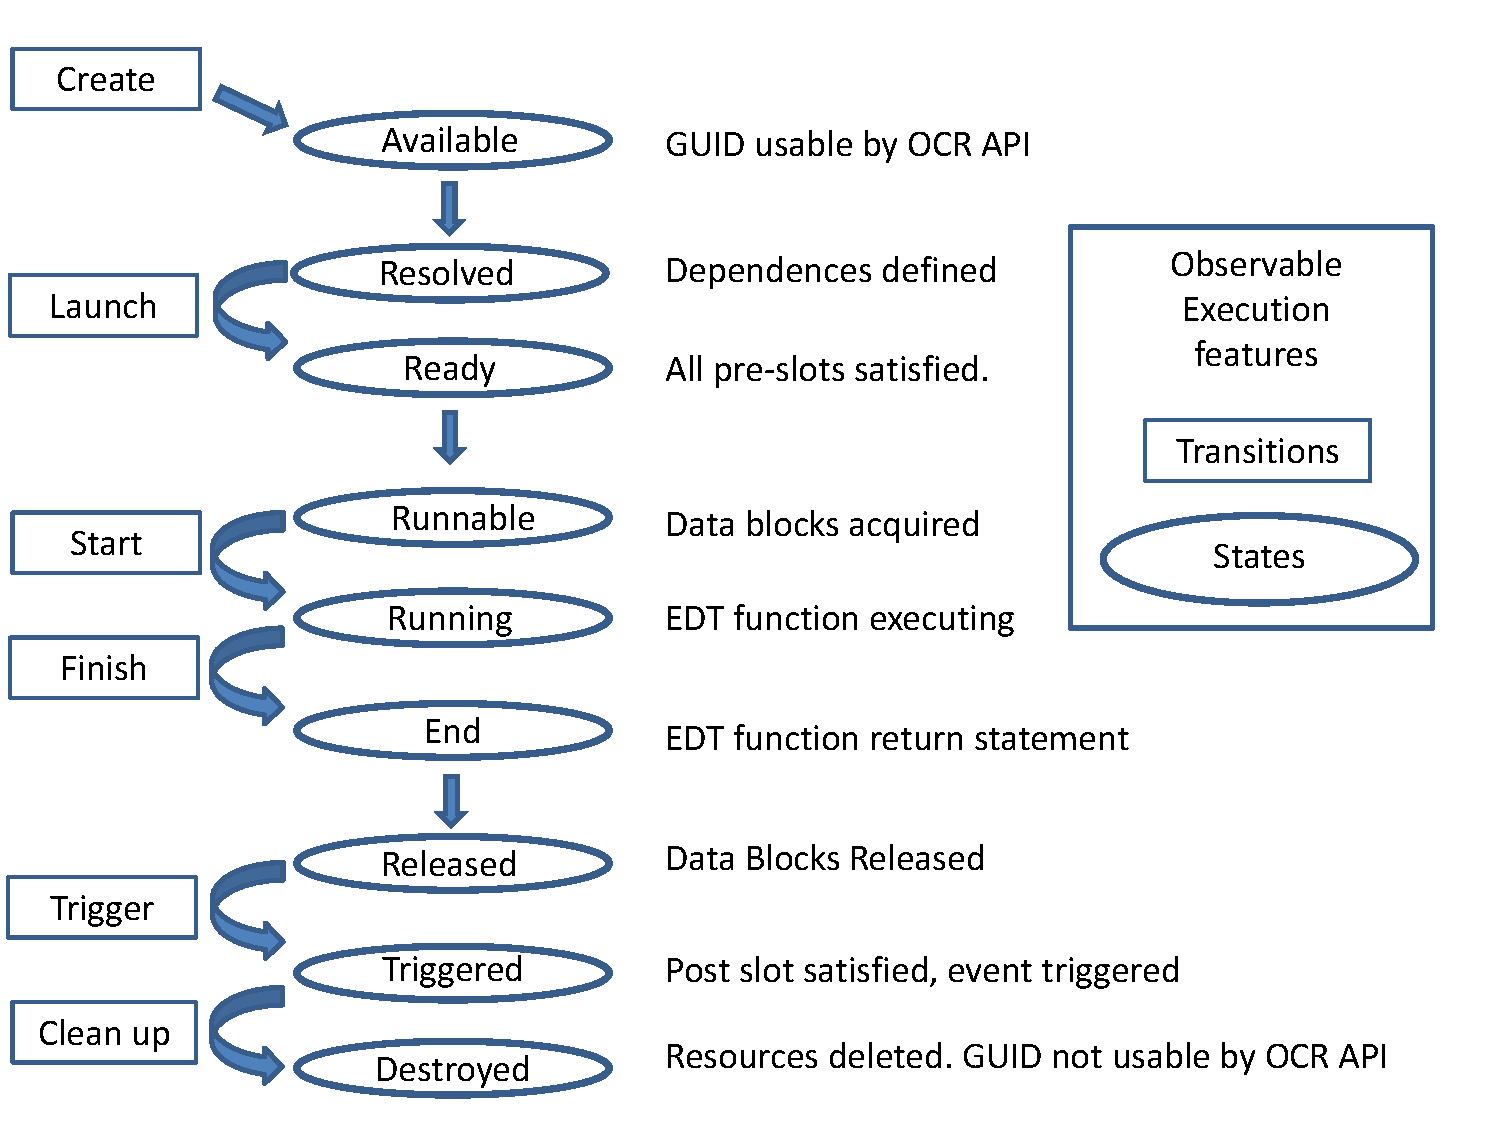
\includegraphics[width=0.9\textwidth]{EDT_exec}
\caption{Observable execution features.}
\label{fig:EDTexec}
\end{figure*}

Normal EDT execution continues until the EDT function returns. The EDT undergoes
a \emph{Finish}\index{EDT transition, finish} transition and the EDT is in
the \emph{End}\index{EDT state, end} state. At some point the EDT will
release the data blocks associated with the EDTs execution and the
EDT enters the \emph{Released}\index{EDT state, released} state.
At this point, any changes made to data blocks will
be available for use by other OCR objects. Later the EDT will
mark its post-slot as satisfied to \emph{Trigger}\index{Trigger} the event
associated with the EDT; thereby becoming a \emph{Triggered} EDT. At
some later point the
system will \emph{Clean-up}\index{EDT transition, clean-up} resources
used by the EDT (including its GUID) and the EDT is destroyed.

Since an EDT is non-blocking, once it
becomes \emph{Runnable} it will run on the OCR platform at some point in the
future. During its run:
\begin{itemize}
\item The EDT can only access data blocks that have been passed in
through its pre-slots as well as any data blocks that the EDT creates
internally. This means that before an EDT starts, the OCR runtime
knows all the data blocks that will be accessed (minus the ones
created within the EDT).

\item The EDT can call into the runtime to create and destroy data
blocks, EDTs and events.

\item The EDT can create \emph{links} between the various OCR
software constructs, termed \emph{dependences}. This is
accomplished through the \code{ocrAddDependence()} function of the OCR
API. The following types of dependences can be created:
\begin{itemize}
\item \emph{Event to Event}: The destination event’s pre-slot is chained
directly to the source event’s post-slot.
For all events but the latch event, this means that the triggering of
the source event will trigger the destination event.

\item \emph{Event to EDT}: One of the destination EDT’s pre-slot is chained
directly to the source event’s post-slot. When the source event is
triggered, this will satisfy the EDT’s pre-slot. If a data block was
associated with the triggering of the source event, that data block
will be made available to the EDT in the dependence array in the
position of the pre-slot. This is a “control + data” dependence. In
the other case, no data block will be made available and the
dependence is akin to a pure control dependence.

\item \emph{Data Block to Event}: Adding a dependence between a data block and an
event is equivalent to satisfying the event with the data block.

\item \emph{Data Block to EDT}: Directly adding a dependence between a data block and
an EDT (a pure data-dependence) immediately satisfies the EDT’s
pre-slot and makes the data block available to the EDT in the
dependence array in the position of the pre-slot.
\end{itemize}

\item The EDT cannot perform any synchronization operations that would
cause it to block inside the body of the task (i.e.\ the EDT must be
non-blocking). The only mechanism for synchronization within OCR is
through the events that link OCR objects, which are explicit to the
runtime.
\end{itemize}

% TODO: Add clarity to the following paragraph on when a programmer
% calls ocrShutdown to terminate even when a few other EDTs haven't
% completed execution, how much is being presumed.

A computation is complete when an EDT terminates the program
(e.g.\ with a call to \code{ocrShutdown()}). Typically, the EDT that
terminates the program is the last EDT in the program DAG, and the
programmer has assured that all other EDTs in the DAG have completed
execution before the function to terminate the program is called.

Since the OCR runtime creates the \code{main()}
function, the programmer does not need to manage the low level
details of initializing and cleanly shutting down OCR.

With both data and tasks conceptually decoupled from their realization
on a computer system, OCR has the flexibility to relocate tasks and data
to respond to failures in the system, achieve a better balance of load
among the processing elements of the computer, or to optimize memory
and energy consumption~\cite{GZCS10,Guo10,CTBCCGYS13,SbBS14}.
This requires that the state of an OCR program can be defined
strictly in terms of which tasks have completed their execution
and the history of updates to data blocks. By saving a log of updates to Data blocks
relative to the tasks that have completed execution, the system can recover
the state of a computation should components of the system fail. This requires,
however, that EDTs execute with transactional semantics.

% This is the end of ch1-exec.tex of the OCR specification.

%
% This is an included file. See the master file for more information.
%

%vivek writes ...
%
%GENERAL COMMENTS:
%
%
%1) A key challenge in defining a memory model is defining the semantics of a data race. All
% memory models usually have the same semantics for data-race-free programs, but vary vastly
% in their definitions of the semantics of data races. For example, I believe that the original
%Release Consistency model had the "memory coherence" assumption which stated that all
% processors see writes to the same location in the same order, which is likely too strong a
%condition for OCR. For a weaker memory model, see Location Consistency (Gao & Sarkar, IEEE ToC 2000).
%

\section{Memory Model}
\index{Memory Model}
\label{sec:MemoryModel}

A memory model defines the values that can be legally observed in
memory when multiple units of execution (e.g.\ processes or threads)
access a shared memory system. The memory model provides programmers
with the tools they need to understand the state of memory, but it
also places restrictions on what a compiler writer can do (e.g.\ which
aggressive optimizations are allowed) and restrictions on what a
hardware designer is allowed to do (e.g.\ the behavior of write
buffers).

To construct a memory model for OCR, we need to present a few
definitions. The operations inside a task execute in a non-blocking
manner. The order of such operations are defined by the
\emph{sequenced-before}\index{sequenced-before} relations defined by
the host C programming language.

When multiple EDTs are running, they execute asynchronously. Usually,
a programmer can make few assumptions about the relative orders of
operations in two different EDTs. At certain points in the execution
of EDTs, however, the OCR program may need to define ordering
constraints. These constraints define
\emph{synchronized-with}\index{synchronized-with} relations.

The ``transitive closure'' of sequenced-before operations inside each
of two EDTs combined with the synchronized-with relations between two
EDTs defines a \emph{happens-before}\index{happens-before}
relationship. For example:
\begin{itemize}
\item if \code{A} is sequenced-before \code{B} in EDT1
\item  if \code{C} is sequenced-before \code{D} in EDT2
\item and  \code{B} is synchronized-with  \code{C} in EDT2
\item then \code{A} happens-before \code{D}.
\end{itemize}
These basic concepts are enough to define the memory model for OCR.


OCR provides a relatively simple memory model. Before an EDT can read
or write a data block, it must first \emph{acquire}\index{Acquire} the data
block. This is not an exclusive relationship by which we mean it is
possible (depending on the mode of the data block in question) for
multiple EDTs to acquire the same data block at the same
time.  When an EDT has finished with a data block and it is ready
to expose any modifications to the data block to other EDTs, it
must \emph{release}\index{Release} that data block.

\begin{quote}
Any function in the OCR runtime that releases a data block must assure
that all loads and stores to the data block occur before the data
block is released and that the release must complete before the
function returns.
\end{quote}

The only way to establish a synchronized-with relation is through the
behavior of events. If the pre-slot of EDT2 is connected to the post-slot
of EDT1, then EDT2 waits for event associated with the post-slot of EDT1 to
trigger. Therefore, the satisfy event from EDT1 synchronizes-with the
triggering of the pre-slot of EDT2. We can establish a happens-before
relationship between the two EDTs if we define the following rule for
OCR.

\begin{quote}
An EDT must complete the release of all of its resources before it
marks its post-event as satisfied.
\end{quote}

An EDT can use data blocks to satisfy events in the body of the task
in addition to the event associated with its post-slot. We can reason
about the behavior of the memory model and establish happens-before
relationship if we define the following rule.

%Vincent's feedback....
%
%"If an EDT uses a Data Block to satisfy an event, all writes to that data block from the EDT must complete
%before the event is triggered.” => I think we already discussed that but I believe you should wait for all the
%db releases that are sequenced-before the satisfy.
%1) This is in case of a db storing guids. db1 has data the edt has written to,  db2 has the guid of db1. %Satisfying ev1 with db2, potentially enables edt2, which spawns edt3 that depends on db1’s guid read from
%db2. With the current rule, db1 may or may not have been released when edt3 acquires it.
%
%db1[0]=1
%db2[0]=db1Guid
%ocrDbRelease(db1)
%ocrDbRelease(db2)
%ocrEventSatisfy(ev1,db2)
%
% TGM responds:
% I submit that since ocrDbRelease(db1) is sequenced before ocrDbRelease(db2) the rules in the memory
%model forces the releases to occur in that order and therefore the model already covers your case.     Can
%you tell me what I'm missing ... because I agree with you completely that the model must force the releases
%to occur in that order prior to the satisfy ... I just think the normal sequenced before relations cover this.
%




\begin{quote}
If an EDT uses a Data Block to satisfy an event, all writes to that data block
from the EDT must complete before the event is triggered.
\end{quote}

Without this rule we can not assume a release operation followed by
satisfying an event defines a sequenced-before relationship that can
be used to establish a happens-before relation.

The core idea in the OCR memory model is that happens-before
relationships are defined in terms of events (the only synchronization
operation in OCR) and the release of OCR objects (such as data
blocks). This is an instance of a \emph{Release
Consistency}\index{Release Consistency} memory model which has the
advantage of being relatively straightforward to apply to OCR
programs.

The safest course for a programmer is to write programs that can be
defined strictly in terms of the release consistency rules. OCR,
however, lets a programmer write programs in which two or more EDTs can
write to a single data block at the same time (or more precisely, the
two EDTs can issue writes in an unordered manner). This may result in a
data race\index{data race} in that the value that is ultimately stored
in memory depends on how a system chooses to schedule operations from
the two EDTs.

Most modern parallel programming languages state that a program that
has a data race\footnote{A \emph{data race} occurs when loads and
stores by two units of execution operate on overlapping memory regions
without a synchronized-with relation to order them} is an illegal
program and the results produced by such a program are undefined.
These programming models then define a complex set of synchronization
constructs and atomic variables so a programmer has the tools needed
to write race-free programs. OCR, however, does not provide any
synchronization constructs beyond the behavior of events. This is not
an oversight. Rather, this restricted synchronization model helps OCR
to better scale on a wider range of parallel computers.

OCR, therefore, allows a programmer to write legal programs that may
potentially contain data races. OCR deals with this situation by
adding two more rules. In both of these rules, we say that address
range $A$ and $B$ are non-overlapping if and only if the set $A_1$ of
8-byte\footnote{The reference to ``8-byte'' words assumes the processing elements
utilize a 64-bit architecture.  For other cases, all references to an 8-byte
word in this specification must be adjusted to match the architecture of the processing elements.}
aligned 8-byte words fully covering $A$ and the set $B_1$ of
8-byte aligned 8-byte words fully covering $B$ do not overlap. For
example, addresses
$0x0$ and $0x7$ overlap (assuming byte level addressing) whereas
$0x0$ and $0x8$ do not.
The first rule deals with the situation of multiple
EDTs writing to a data block with non-overlapping address ranges.
\begin{quote}
If two EDTs write to a single data block without a well defined order,
if the address ranges of the writes do not overlap, the correct result
of each write operation must appear in memory.
\end{quote}

This behavior may seem obvious making it trivial for a system to
support. However, when addresses are distinct but happen to share the
same cache lines or when aggressive optimization of writes occur
through write buffers, an implementation could mask the updates from
one of the EDTs if this rule were not defined in the OCR
specification.

The last rule addresses the case of overlapping address ranges.  Assume that
a system writes values to memory at an atomicity of N-bytes.  This defines
the fundamental store-atomicity for the system\index{store-atomicity}.
\begin{quote}
If two EDTs write to a single data block without a well defined order,
if the address ranges of the writes overlap, the results written to
memory must correspond to one of the legal interleavings of statements
from the two EDTs at an N-byte aligned granularity. Overlapping writes
to non-aligned or smaller than N-byte granularity are not defined.
\end{quote}
For systems that do not provide store-atomicity at any level, N would be 0
and the above rule states that unordered writes to overlapping address
ranges are undefined.
This rule is the well known \emph{sequential consistency}\index{sequential
consistency} rule. It states that the actual result appearing in
memory may be nondeterministic, but it will be well defined and it
will correspond to values from one EDT or the other.

Release consistency remains the safest and best approach to use in
writing OCR programs. It is conceivable that some of the more
difficult rules may be relaxed in future versions of OCR (especially
the sequential consistency rule), but the relaxed consistency model
will almost assuredly always be supported by OCR.

Any memory in OCR that can be accessed by multiple EDTs resides in data blocks.  As
discussed in section~\ref{sec:datablocks} there
are four access modes for the data blocks in OCR. The modes and how they
interact with the OCR memory model are listed as follows.
\begin{itemize}

\item \emph{Read-Write} (default mode)\index{Data Block, read-write}: The EDT may read
and write to the data block.  Multiple EDTs may
write to the same data block at the same time with values constrained according to the
rules in the OCR memory model.

\item \emph{Exclusive write}\index{Data Block, exclusive write}: The
EDT requires that it is the only EDT that can commit write operations to a data block at a
given time.  Writes must follow a sequential total order; i.e.\ when more than one EDT is writing
to a data block in exclusive write mode, all the writes from one EDT must complete before
a subsequent EDT can acquire and then write to the data block.  This serializes the execution of
EDTs that acquire data blocks in exclusive write mode.

\item \emph{Read only}\index{Data Block, read only}: The EDT
will only read from the Data Block. The OCR Runtime does
not restrict the ability of other EDTs to write to the data block.  The
visibility of those writes are undefined; i.e.\ an implementation may
choose whether or not to make writes by other EDTs visible.

\item \emph{Constant}\index{Data Block,constant}: The EDT will only read from the
data block and the OCR runtime will assure that once the data block is acquired,
writes from other EDTs will not be visible.

\end{itemize}


% This is the end of ch1-memory.tex of the OCR specification.
%%%%%
\section{Organization of this document}
\label{sec:Organization of this document}
% Vivek writes ... Add a new section on OCR semantics that covers properties such as
% deadlock, data races, functional determinism, and structural determinism.
%
%  TGM responds ... I am confused by what you are asking for.  This is a specfication.
%  Do these concepts really belong here?

The remainder of this document is structured as follows:

\begin{itemize}
\item Chapter~\ref{chap:OCRAPI} defines the OCR Application Programming Interface.

\item Appendix~\ref{chap:Appendix A} contains a set of pedagogical examples.

\item Appendix~\ref{chap:Appendix B} contains a set of proposed OCR Extensions.

\item Appendix~\ref{chap:Appendix C} contains notes specific to current implementations of OCR.

\item Appendix~\ref{chap:Appendix D} documents the ``change history''
  for OCR and this specification.
\end{itemize}


% This is the end of ch1-main.tex of the OCR specification.


    % This is an included file. See the master file for more information.
%

% This is an included file. See the master file for more information.
%

% this name sucks ... just call it OCR API
\chapter{The OCR API }
\label{chap:OCRAPI}

This chapter describes the syntax and behavior of the OCR API functions, and is divided
into the following sections:
\begin{itemize}
\item The core types, macros and error codes used in OCR.
(\specref{sec:OCRtypesmacros})

\item A description of OCR main entry point: \code{mainEdt}.
(\specref{sec:mainEDT})

\item Supporting functions.
(\specref{sec:supportFuncs})

\item Functions to create, destroy, and otherwise manage the contents of OCR data blocks.
(\specref{sec:OCRDataBlockManagement})

\item Functions to manage events in OCR.
(\specref{sec:OCREventManagement})

\item Functions to create and destroy tasks in OCR.
(\specref{sec:OCRTaskManagement})

\item Functions to manage dependences between OCR objects.
(\specref{sec:OCRDependenceManagement})
\end{itemize}

Types, constants, function prototypes and anything else required to use the
OCR API are made available through the \code{ocr.h} include file. You do not
need to include any other files unless using extended or experimental
features (described in the appendices).
% This is the end of ch2-intro.tex of the OCR specification.

% This is an included file. See the master file for more information.
%

\section{OCR core types, macros, and error codes}
\index{OCR types, macros, and error codes}
\label{sec:OCRtypesmacros}

The OCR Application Programming Interface (API) is defined in terms of a
C language binding. The functions comprising the OCR API make use of a number of
basic data types defined in the include file \code{ocr.h}.
%%
\paragraph*{Base low-level types}
The lowest level data types are defined in terms of the following C typedef
statements:
\begin{itemize}
\item \hypertarget{type_u64}{\code{typedef uint64\_t u64}} 64-bit unsigned integer;
\item \hypertarget{type_u32}{\code{typedef uint32\_t u32}} 32-bit unsigned integer;
\item \hypertarget{type_u16}{\code{typedef uint16\_t u16}} 16-bit unsigned integer;
\item \hypertarget{type_u8}{\code{typedef uint8\_t u8}} 8-bit unsigned integer;
\item \hypertarget{type_s64}{\code{typedef int64\_t s64}} 64-bit signed integer;
\item \hypertarget{type_s32}{\code{typedef int32\_t s32}} 32-bit signed integer;
\item \hypertarget{type_s8}{\code{typedef int8\_t s8}} 8-bit signed integer;
\item \hypertarget{type_bool}{\code{typedef u8 bool}} 8-bit boolean.
\item \hypertarget{type_ocrEdtDep_t}{\code{ocrEdtDep\_t}}: Type of
  dependences as passed into the EDTs. It contains at least two fields
  that can be used by the programmer: \code{guid} which contains the
  GUID of the data block passed in and \code{ptr} which contains a
  pointer to the aforementioned data block.
\end{itemize}
%%
\paragraph*{OCR opaque types}
In addition to these low level types, OCR defines a number of opaque data types
to manage OCR objects and to interact with the OCR environment:
\begin{itemize}
\item \hypertarget{type_ocrGuid_t}{\code{ocrGuid\_t}}: Opaque handle used to
reference all OCR objects. An \code{ocrGuid\_t} is truly opaque and
the user cannot assume that it is of a given size;
\end{itemize}
%%
\paragraph*{Other constants}
The C API for OCR makes use of a set of basic macros defined
inside \code{ocr.h}:
\begin{itemize}
\item \code{\#define true 1};
\item \code{\#define TRUE 1};
\item \code{\#define false 0};
\item \code{\#define FALSE 0};
\item \code{\#define NULL\_HINT}: A NULL pointer to ocrHint\_t. This value cannot
  be assumed to be equal to zero.
\item \code{\#define NULL\_GUID}: A NULL ocrGuid\_t. This value cannot
  be assumed to be equal to zero. In other words, a programmer should
  explicitly test for equality to NULL\_GUID.
\item \code{\#define UNINITIALIZED\_GUID}: An Unitialized GUID (ie: never set);
\item \code{\#define ERROR\_GUID}: An invalid GUID.
\end{itemize}
%%
\paragraph*{OCR error codes}
The OCR error codes are derived from standard error codes. They are defined
internally to limit OCR's dependence on standard libraries. Most functions in the
OCR API will return a status code where 0 signifies successful completion. A non-zero
return code will be one of the following error codes. These codes are found
in the \code{ocr-errors.h} include file and described in Table~\ref{tab:errorcodes}.
Since OCR aims to be as asynchronous as possible, it is not always
possible or advisable to return an error code as soon as called
function returns. A compliant implementation may therefore not detect
all possible errors. Future revisions of this specification will
provide a more robust mechanism for more accurately checking for error conditions.
\tablefirsthead{%
\hline
\textsf{\textbf{Error code}} & \textsf{\textbf{Generic Interpretation}}\\
\hline \\[-3ex]
}
\tablehead{%
\multicolumn{2}{l}{\small\sl table continued from previous page}\\
\hline
\textsf{\textbf{Error code}} & \textsf{\textbf{Generic Interpretation}}\\
\hline \\[-3ex]
}
\tabletail{%
\hline\\[-1ex]
\multicolumn{2}{l}{\small\sl table continued on next page}\\
}
\tablelasttail{\hline}
\begin{supertabular}{p{1.25in} p{2.75in}}
\label{tab:errorcodes}
\plc{OCR\_EPERM} & Operation not permitted\\
\plc{OCR\_ENOENT} & No such file or directory\\
\plc{OCR\_EINTR} & Interrupted OCR runtime call\\
\plc{OCR\_EIO} & I/O error\\
\plc{OCR\_ENXIO} & No such device or address\\
\plc{OCR\_E2BIG} & Argument list too long\\
\plc{OCR\_ENOEXEC} & Exec format error\\
\plc{OCR\_EAGAIN} & Try again\\
\plc{OCR\_ENOMEM} & Out of memory\\
\plc{OCR\_EACCES} & Permission denied\\
\plc{OCR\_EFAULT} & Bad address\\
\plc{OCR\_EBUSY} & Device or resource busy\\
\plc{OCR\_ENODEV} & No such device\\
\plc{OCR\_EINVAL} & Invalid argument\\
\plc{OCR\_ENOSPC} & No space left on device\\
\plc{OCR\_ESPIPE} & Illegal seek\\
\plc{OCR\_EROFS} & Read-only file system\\
\plc{OCR\_EDOM} & Math argument out of domain of func\\
\plc{OCR\_ERANGE} & Math result not representable\\
\plc{OCR\_ENOSYS} & Function not implemented\\
\plc{OCR\_ENOTSUP} & Function is not supported\\
\plc{OCR\_EGUIDEXISTS} & The objected referred to by GUID already exists\\
\plc{OCR\_EACQ} & Data block is already acquired\\
\plc{OCR\_EPEND} & Operation is pending\\
\plc{OCR\_ECANCELED} & Operation canceled\\
\end{supertabular}
%%%%%%%%%%%%%%%%%%%%%%%%%%%%%%%%%%%%%%%%%%%%%%%%
%% The OCR Main EDT
%%%%%%%%%%%%%%%%%%%%%%%%%%%%%%%%%%%%%%%%%%%%%%%%
\hypertarget{func_mainEdt}{
\section{OCR entry point: \code{mainEdt}}}
\label{sec:mainEDT}

An OCR program's single point of entry is the user-defined main EDT (\code{mainEdt()}).
This EDT has a function prototype that is identical to any other EDT; its parameters
and dependences are however special: the main EDT has no parameters and has a single
input data block that encodes the arguments passed to the program from the
command line. The arguments can be accessed using \hyperlink{func_getArgc}{\code{getArgc()}}
and \hyperlink{func_getArgv}{\code{getArgv()}}.

\begin{boxedcode}
\plc{ocrGuid\_t mainEdt(u32 paramc, u64* paramv, u32 depc, ocrEdtDep\_t depv[])}
\end{boxedcode}

\begin{DoxyParams}[1]{Parameters}
\mbox{\tt in} & \code{paramc} & Parameters count will always be 0.\\
\hline
\mbox{\tt in} & \code{paramv} & Parameter version will always be NULL.\\
\hline
\mbox{\tt in} & \code{depc} & Dependence count will always be 1.\\
\hline
\mbox{\tt in} & \code{depv} & Dependence vector will have exactly 1 entry
containing a data block that encodes the command line arguments.\\
\hline
\end{DoxyParams}

\returns
\code{mainEdt} returns a \hyperlink{type_ocrGuid_t}{\code{ocrGuid\_t}} which is
ignored by the runtime. The returned value of an OCR program is set using
\hyperlink{func_ocrShutdown}{\code{ocrShutdown()}} or \hyperlink{func_ocrAbort}{
  \code{ocrAbort()}}.
%%%%%%%%%%%%%%%%%%%%%%%%%%%%%%%%%%%%%%%%%%%%%%%%
%% Supporting Functions
%%%%%%%%%%%%%%%%%%%%%%%%%%%%%%%%%%%%%%%%%%%%%%%%
\section{Supporting functions}
\label{sec:supportFuncs}

OCR provides a set of basic capabilities to support a program execution environment,
handled through the following functions.

\subsection*{Functions}
\begin{DoxyCompactItemize}
\item
  void \hyperlink{func_ocrShutdown}{\code{ocrShutdown}}(void)
    \begin{DoxyCompactList}
      \small\item \emph{Called by an EDT to indicate the normal end of an OCR program.}
    \end{DoxyCompactList}
\item
  void \hyperlink{func_ocrAbort}{\code{ocrAbort}}(\hyperlink{type_u8}{u8} errorCode)
    \begin{DoxyCompactList}
      \small\item \emph{Called by an EDT to indicate an abnormal end of an OCR program.}
    \end{DoxyCompactList}
\item
  \hyperlink{type_u64}{u64} \hyperlink{func_getArgc}{\code{getArgc}}(void $\ast$dbPtr)
    \begin{DoxyCompactList}
      \small\item \emph{Retrieves the traditional `argc' value from
        \hyperlink{func_mainEdt}{\code{mainEdt()}}'s input data block.}
    \end{DoxyCompactList}
\item
  char $\ast$ \hyperlink{func_getArgv}{\code{getArgv}}(void $\ast$dbPtr,
  \hyperlink{type_u64}{u64} count)
    \begin{DoxyCompactList}
      \small\item \emph{Retrieves the `count' argument from
        \hyperlink{func_mainEdt}{\code{mainEdt()}}'s input data block.}
    \end{DoxyCompactList}
\item
  \hyperlink{type_u32}{u32} \hyperlink{func_PRINTF}{\code{PRINTF}}(const char $\ast$format, ...)
    \begin{DoxyCompactList}
      \small\item \emph{\code{printf()} equivalent for OCR.}
    \end{DoxyCompactList}
\end{DoxyCompactItemize}
%
% ocrShutdown
%
\hypertarget{func_ocrShutdown}{
  \index{Supporting functions@{Supporting function}!ocr\-Shutdown@{ocr\-Shutdown}}
  \subsection[{ocr\-Shutdown}]{\setlength{\rightskip}{0pt plus 5cm}void ocr\-Shutdown(
)}}
\label{func_ocrShutdown}

The user is responsible for indicating the end of an OCR program using an explicit
shutdown call (either this function or \hyperlink{func_ocrAbort}{\code{ocrAbort()}}).
Any EDTs which have not reached the \emph{runnable} state will never be executed.
EDTs in the \emph{runnable} or \emph{ready} state may or may not execute.

\begin{DoxyNote}{Note}
Program behavior after this call is undefined. Specifically:
\begin{itemize}
  \item The statements in the calling EDT \emph{after} this function
    call may or may not be executed;
  \item EDTs in the \emph{runnable} or \emph{ready} state may or may not
    execute.
\end{itemize}

Although most programs will choose to call \code{ocrShutdown()} in the ``last'' EDT,
OCR specifically allows another EDT to call \code{ocrShutdown()} to support, for
example, a computation of the type ``find-first-of''; in such a computation, the
program can successfully complete even if all EDTs have not executed.
\end{DoxyNote}
%
% ocrAbort
%
\hypertarget{func_ocrAbort}{
  \index{Supporting functions@{Supporting functions}!ocr\-Abort@{ocr\-Abort}}
  \subsection[{ocr\-Abort}]{\setlength{\rightskip}{0pt plus 5cm}void ocr\-Abort(
\begin{DoxyParamCaption}
\item[{{\bf u8}}]{error\-Code}
\end{DoxyParamCaption}
)}}
\label{func_ocrAbort}

This function is very similar to \hyperlink{func_ocrShutdown}{\code{ocrShutdown()}}
except that it allows for the return of a non-zero value.

The abort error code is passed back to the runtime and its handling is
implementation dependent

\begin{DoxyParams}[1]{Parameters}
\mbox{\tt in} & \code{errorCode} & User defined error code returned to the runtime.\\
\hline
\end{DoxyParams}

\descr
See notes in Section~\ref{func_ocrShutdown}.
%
% getArgc
%
\hypertarget{func_getArgc}{
  \index{Supporting functions@{Supporting function}!get\-Argc@{get\-Argc}}
  \subsection[{get\-Argc}]{\setlength{\rightskip}{0pt plus 5cm}{\bf u64} get\-Argc(
\begin{DoxyParamCaption}
\item[{void $\ast$}]{db\-Ptr}
\end{DoxyParamCaption}
)}}
\label{func_getArgc}

Returns the number of arguments (traditionally called `argc') passed to the OCR program.
The value is extracted from the unique data block passed to \hyperlink{func_mainEdt}{\code{mainEdt}}.

\begin{DoxyParams}[1]{Parameters}
\mbox{\tt in} & \code{dbPtr} & Pointer to the start of the argument data block\\
\hline
\end{DoxyParams}

\returns
The number of arguments passed to the OCR program on the command line

\descr
When starting, the first EDT (called \hyperlink{func_mainEdt}{\code{mainEdt}}) is
passed a single input data block which encodes the arguments passed to the main
program:
\begin{DoxyItemize}
\item The first 8 bytes encode `argc';
\item The following `argc' 8-byte values encode the offset
  from the start of the data block to the arguments;
\item The arguments are then appended as NULL terminated
  character arrays.
\end{DoxyItemize}
%
% getArgv
%
\hypertarget{func_getArgv}{
  \index{Supporting functions@{Supporting function}!get\-Argv@{get\-Argv}}
  \subsection[{get\-Argv}]{\setlength{\rightskip}{0pt plus 5cm}{\bf char $\ast$} get\-Argv(
\begin{DoxyParamCaption}
\item[{void $\ast$}]{db\-Ptr}
\item[{{\bf u64}}]{count}
\end{DoxyParamCaption}
)}}
\label{func_getArgv}

Returns the `count' argument passed to the OCR program.
The value is extracted from the unique data block passed to \hyperlink{func_mainEdt}{\code{mainEdt}}.

\begin{DoxyParams}[1]{Parameters}
\mbox{\tt in} & \code{dbPtr} & Pointer to the start of the argument data block\\
\hline
\mbox{\tt in} & \code{count} & Index of the argument to extract\\
\hline
\end{DoxyParams}

\returns
A NULL terminated string corresponding to \code{argv[count]}.

\descr
See Section~\ref{func_getArgc} for details.
\begin{DoxyNote}{Note}
Attempting to extract an argument with \code{count} greater or equal to the value
returned by \hyperlink{func_getArgc}{\code{getArgc}} will result in undefined
behavior.
\end{DoxyNote}
%
% PRINTF
%
\hypertarget{func_PRINTF}{
  \index{Supporting functions@{Supporting function}!PRINTF@{PRINTF}}
  \subsection[{PRINTF}]{\setlength{\rightskip}{0pt plus 5cm}{\bf u32} PRINTF(
\begin{DoxyParamCaption}
\item[{const char $\ast$}]{fmt}
\item[{}]{...}
\end{DoxyParamCaption}
)}}
\label{func_PRINTF}

A platform independent limited \code{printf} functionality.

\begin{DoxyParams}[1]{Parameters}
\mbox{\tt in} & \code{fmt} & NULL terminated C format string containing the
format of the output string\\
\hline
\mbox{\tt in} & \code{...} & A variable length list of arguments in agreement with
\code{fmt}\\
\hline
\end{DoxyParams}

\returns
This function returns the number of bytes written out as a
\hyperlink{type_u32}{\code{u32}}.

\descr
OCR must support a wide variety of platforms including simulators that emulate
real systems. Often, core functionality provided by standard C libraries are not
available on all platforms, and, as a result, an OCR program cannot depend on
these functions. There was one case, however, where it was felt support was
critical: basic printf. This function supports basic printing functionality
and supports the following format specifiers:
\begin{itemize}
\item Strings using \code{\%s};
\item 32-bit integers using \code{\%d}, \code{\%u}, \code{\%x} and \code{\%X};
\item 64-bit integers using \code{\%ld}, \code{\%lu}, \code{\%lx}, \code{\%lX},
  and versions with two `l';
\item 64-bit pointers using \code{\%p};
\item Floating point numbers using \code{\%f}, \code{\%e} and \code{\%E};
\item The `\#' flag is supported for \code{\%x}, \code{\%lx} and \code{\%llx};
\item Precision modifiers are also supported for \code{\%f}, \code{\%e} and \code{\%E}.
\end{itemize}

\begin{DoxyNote}{Note}
A conformant implementation may limit the number of characters in the
output string.
\end{DoxyNote}
%%%%%%%%%%%%%%%%%%%%%%%%%%%%%%%%%%%%%%%%%%%%%%%%
%% GUID MANAGEMENT API
%%%%%%%%%%%%%%%%%%%%%%%%%%%%%%%%%%%%%%%%%%%%%%%%
\section{GUID management}
\index{GUID management API}
\label{sec:OCRGuidManagement}

GUIDs are opaque values used to uniquely identify OCR objects. In
previous versions of OCR, GUID values could be safely cast to 64-bit
values. To preserve the runtime's freedom in encoding information into
GUIDs, users can no longer rely on the ability to convert GUIDs to
64-bit values and must instead use the provided functions to
manipulate GUIDs.

\subsection*{Functions}
\begin{DoxyCompactItemize}
\item
  \hyperlink{type_bool}{bool} \hyperlink{func_ocrGuidIsNull}
            {\code{ocrGuidIsNull}}(\hyperlink{type_ocrGuid_t}{ocr\-Guid\-\_\-t} guid)
    \begin{DoxyCompactList}
      \small\item \emph{Checks if the GUID provided is equivalent to NULL\_GUID.}
    \end{DoxyCompactList}
\item
  \hyperlink{type_bool}{bool} \hyperlink{func_ocrGuidIsUninitialized}
            {\code{ocrGuidIsUninitialized}}(\hyperlink{type_ocrGuid_t}{ocr\-Guid\-\_\-t} guid)
    \begin{DoxyCompactList}
      \small\item \emph{Checks if the GUID provided is equivalent to UNINITIALIZED\_GUID.}
    \end{DoxyCompactList}
\item
  \hyperlink{type_bool}{bool} \hyperlink{func_ocrGuidIsError}
            {\code{ocrGuidIsError}}(\hyperlink{type_ocrGuid_t}{ocr\-Guid\-\_\-t} guid)
    \begin{DoxyCompactList}
      \small\item \emph{Checks if the GUID provided is equivalent to ERROR\_GUID.}
    \end{DoxyCompactList}
\item
  \hyperlink{type_bool}{bool} \hyperlink{func_ocrGuidIsEq}
            {\code{ocrGuidIsEq}}(\hyperlink{type_ocrGuid_t}{ocr\-Guid\-\_\-t} guid1,
    \hyperlink{type_ocrGuid_t}{ocr\-Guid\-\_\-t} guid2)
    \begin{DoxyCompactList}
      \small\item \emph{Checks if the two GUIDs provided are equivalent.}
    \end{DoxyCompactList}
\item
  \hyperlink{type_bool}{bool} \hyperlink{func_ocrGuidIsLt}
            {\code{ocrGuidIsLt}}(\hyperlink{type_ocrGuid_t}{ocr\-Guid\-\_\-t} guid1,
    \hyperlink{type_ocrGuid_t}{ocr\-Guid\-\_\-t} guid2)
    \begin{DoxyCompactList}
      \small\item \emph{Checks if guid1 is less than guid2.}
    \end{DoxyCompactList}
\end{DoxyCompactItemize}

%
%  ocrGuidIsNull
%
\hypertarget{func_ocrGuidIsNull}{
  \index{GUID management@{GUID management}!ocr\-Guid\-Is\-Null@{ocr\-Guid\-Is\-Null}}
  \subsection[{ocr\-Guid\-Is\-Null}]{\setlength{\rightskip}{0pt plus 5cm}{\bf bool} ocr\-Guid\-Is\-Null(
\begin{DoxyParamCaption}
\item[{{\bf ocr\-Guid\-\_\-t}}]{guid }
\end{DoxyParamCaption}
)}}
\label{func_ocrGuidIsNull}

NULL\_GUID is a special value representing a NULL ocrGuid\_t. This
returns true if \code{guid} is equivalent to NULL\_GUID.

\begin{DoxyParams}[1]{Parameters}
\mbox{\tt in}  & \code{guid} & GUID to be evaluated.\\
\hline
\end{DoxyParams}

\returns
A boolean:
\begin{DoxyItemize}
\item true: guid is equivalent to NULL\_GUID
\item false: guid is not equivalent to NULL\_GUID
\end{DoxyItemize}

%
%  ocrGuidIsUninitialized
%
\hypertarget{func_ocrGuidIsUninitialized}{
  \index{GUID management@{GUID management}!ocr\-Guid\-Is\-Uninitialized@{ocr\-Guid\-Is\-Uninitialized}}
  \subsection[{ocr\-Guid\-Is\-Uninitialized}]{\setlength{\rightskip}{0pt plus 5cm}{\bf bool} ocr\-Guid\-Is\-Uninitialized(
\begin{DoxyParamCaption}
\item[{{\bf ocr\-Guid\-\_\-t}}]{guid }
\end{DoxyParamCaption}
)}}
\label{func_ocrGuidIsUninitialized}

UNINITIALIZED\_GUID is a special value representing an uninitialized ocrGuid\_t.
This function checks if the GUID provided is equivalent to UNINITIALIZED\_GUID.

\begin{DoxyParams}[1]{Parameters}
\mbox{\tt in}  & \code{guid} & GUID to be evaluated.\\
\hline
\end{DoxyParams}

\returns
A boolean:
\begin{DoxyItemize}
\item true: guid is equivalent to UNINITIALIZED\_GUID
\item false: guid is not equivalent to UNINITIALIZED\_GUID
\end{DoxyItemize}

%
%  ocrGuidIsError
%
\hypertarget{func_ocrGuidIsError}{
  \index{GUID management@{GUID management}!ocr\-Guid\-Is\-Error@{ocr\-Guid\-Is\-Error}}
  \subsection[{ocr\-Guid\-Is\-Error}]{\setlength{\rightskip}{0pt plus 5cm}{\bf bool} ocr\-Guid\-Is\-Error(
\begin{DoxyParamCaption}
\item[{{\bf ocr\-Guid\-\_\-t}}]{guid }
\end{DoxyParamCaption}
)}}
\label{func_ocrGuidIsError}

ERROR\_GUID is a special value representing a invalid ocrGuid\_t. This
function checks if the GUID provided is equivalent to ERROR\_GUID.

\begin{DoxyParams}[1]{Parameters}
\mbox{\tt in}  & \code{guid} & GUID to be evaluated.\\
\hline
\end{DoxyParams}

\returns
A boolean:
\begin{DoxyItemize}
\item true: guid value is equivalent to ERROR\_GUID
\item false: guid value is not equivalent to ERROR\_GUID
\end{DoxyItemize}

%
%  ocrGuidIsEq
%
\hypertarget{func_ocrGuidIsEq}{
  \index{GUID management@{GUID management}!ocr\-Guid\-Is\-Eq@{ocr\-Guid\-Is\-Eq}}
  \subsection[{ocr\-Guid\-Is\-Eq}]{\setlength{\rightskip}{0pt plus 5cm}{\bf bool} ocr\-Guid\-Is\-Eq(
\begin{DoxyParamCaption}
\item[{{\bf ocr\-Guid\-\_\-t}}]{guid1, }
\item[{{\bf ocr\-Guid\-\_\-t}}]{guid2  }
\end{DoxyParamCaption}
)}}
\label{func_ocrGuidIsEq}

This function checks if guid1 and guid2 are equivalent.

\begin{DoxyParams}[1]{Parameters}
\mbox{\tt in}  & \code{guid1} & GUID to be evaluated.\\
\hline
\mbox{\tt in}  & \code{guid2} & GUID to be evaluated.\\
\hline
\end{DoxyParams}

\returns
A boolean:
\begin{DoxyItemize}
\item true: guid1 and guid2 are equivalent
\item false: guid1 and guid2 are not equivalent
\end{DoxyItemize}

%
%  ocrGuidIsLt
%
\hypertarget{func_ocrGuidIsLt}{
  \index{GUID management@{GUID management}!ocr\-Guid\-Is\-Lt@{ocr\-Guid\-Is\-Lt}}
  \subsection[{ocr\-Guid\-Is\-Lt}]{\setlength{\rightskip}{0pt plus 5cm}{\bf bool} ocr\-Guid\-Is\-Lt(
\begin{DoxyParamCaption}
\item[{{\bf ocr\-Guid\-\_\-t}}]{guid1, }
\item[{{\bf ocr\-Guid\-\_\-t}}]{guid2  }
\end{DoxyParamCaption}
)}}
\label{func_ocrGuidIsLt}

This function checks if guid1 is less than guid2.

\begin{DoxyParams}[1]{Parameters}
\mbox{\tt in}  & \code{guid1} & GUID to be evaluated.\\
\hline
\mbox{\tt in}  & \code{guid2} & GUID to be evaluated.\\
\hline
\end{DoxyParams}

\returns
A boolean:
\begin{DoxyItemize}
\item true: guid1 is less than guid2
\item false: guid1 is greater than or equal to guid2
\end{DoxyItemize}

\subsection{Macros for printing GUIDs}
It is often desirable in both applications and runtime to
print the value of a GUID for debugging purposes. Under previous
assumptions that GUIDs were \code{unsigned long} values, they were printed using
the \code{"\%PRIx64"} placeholder. Since GUIDs are opaque, their size
cannot be assumed and format specifiers are therefore provided to
properly print GUIDs.

\begin{itemize}
\item \code{GUIDF}
  \small \emph{Format placeholder representing a GUID.}
\item \code{GUIDA(guid)}
  \small \emph{Expands guid value into format arguments
  corresponding to the GUIDF format placeholder.}
\end{itemize}

The following snippet shows how to print a GUID:
\begin{ocrsnip}
PRINTF("DB Guid "GUIDF" acquired by "GUIDF"\n", GUIDA(db.guid), GUIDA(edt.guid));
\end{ocrsnip}

Note that the \code{GUIDF} format placeholder macro may actually expand into
multiple concrete format placeholders. Likewise, the \code{GUIDA} macro may
expand its single GUID argument into multiple arguments for a format function's
argument list, corresponding to the number of concrete placeholders included
by the \code{GUIDF} macro.
%%%%%%%%%%%%%%%%%%%%%%%%%%%%%%%%%%%%%%%%%%%%%%%%
%% Data Block Management
%%%%%%%%%%%%%%%%%%%%%%%%%%%%%%%%%%%%%%%%%%%%%%%%
\section{Data block management}
\index{Data block management APIs}
\label{sec:OCRDataBlockManagement}

Data blocks are the only form of non-\/ephemeral storage and are therefore
the only way to ``share'' data between E\-D\-Ts. Conceptually, data blocks
are contiguous chunks of memory that have a start address and a size.
They also have the following characteristics\-:
\begin{itemize}
\item all memory within the data block is accessible from the start-\/address
  using an offset (ie\-: addresses \mbox{[}start-\/address; start-\/address+size\mbox{[}
  uniquely and totally address the entire data-\/block);
\item a data block is non-\/overlapping with other distinct data blocks
\item the pointer to the start of a data block is only valid between the start
of the E\-D\-T (or the data block creation) and the corresponding \code{ocrDbRelease}
(or the end of the E\-D\-T).
\end{itemize}

The following macros and enums are used with OCR data blocks.
\begin{itemize}
\item \hypertarget{type_ocrInDbAllocator_t}{\code{enum ocrInDbAllocator\_t}} containing:
  \begin{itemize}
  \item \code{NO\_ALLOC} The data block is not used as a heap
  \end{itemize}
\item \hypertarget{type_ocrDbAccessMode_t}{\code{enum ocrDbAccessMode\_t}}
  containing the four access modes. The
  meaning of the access modes is given in Section~\ref{sec:datablocks}:
  \begin{itemize}
    \item \code{DB\_MODE\_RW}
    \item \code{DB\_MODE\_EW}
    \item \code{DB\_MODE\_RO}
    \item \code{DB\_MODE\_CONST}
  \end{itemize}
\item \code{DB\_DEFAULT\_MODE} which is an alias of \code{DB\_MODE\_RW}
\item \code{DB\_PROP\_NONE} which specifies no special properties on the data block
\item \code{DB\_PROP\_NO\_ACQUIRE} which specifies that the data block should
  not be acquired on creation
\end{itemize}

%% This is a repeat of sec:datablocks. Keeping for now commented.

%% These are the modes with which an EDT can access a data block.
%% OCR currently supports four modes:
%% \begin{itemize}
%% \item \code{DB\_MODE\_RW} Read-Write (default mode): The EDT is stating that it
%% may read from and write-to the data block. The user is responsible for
%% synchronizing between EDTs that could potentially write to the same data block
%% concurrently.
%% \item \code{DB\_MODE\_EW} Exclusive-Write (EW): The EDT requires that it be
%% the only one writing to the data block. The runtime will not schedule any other
%% EDT that accesses the same data block in RW or EW mode concurrently.
%% This can limit parallelism.
%% \item \code{DB\_MODE\_RO} Read-Only: The EDT is stating that it will only read
%% from the data block. The runtime will not enforce this restriction but the
%% visibility of any writes done by the EDT is undefined. The runtime also does
%% not guarantee that concurrent writes to the data block from other EDTs
%% will not be visible. In other words, another concurrent EDT in EW or RW mode may
%% concurrently access the data block and modify it while this EDT is accessing it in
%% RO mode.
%% \item \code{DB\_MODE\_CONST} Constant: Similarly to the RO mode, the EDT is
%% again stating that it will not write to the data block. In this mode, however,
%% the runtime guarantees that the data block seen by the EDT will not be modified
%% by other concurrent EDTs. Similarly to the RO mode, the visibility of any writes
%% by this EDT (in violation of the ``contract'') is undefined.
%% \end{itemize}

\subsection*{Functions}
\begin{DoxyCompactItemize}
\item
  \hyperlink{type_u8}{u8} \hyperlink{func_ocrDbCreate}
            {\code{ocrDbCreate}}(\hyperlink{type_ocrGuid_t}{ocr\-Guid\-\_\-t} $\ast$db,
    void $\ast$$\ast$addr, \hyperlink{type_u64}{u64} len, \hyperlink{type_u16}{u16} flags,
    \hyperlink{type_ocrHint_t}{ocr\-Hint\-\_\-t} $\ast$hint,
    \hyperlink{type_ocrInDbAllocator_t}{ocr\-In\-Db\-Allocator\-\_\-t} allocator)
    \begin{DoxyCompactList}
      \small\item \emph{Request the creation of a data block.}
    \end{DoxyCompactList}
\item
  \hyperlink{type_u8}{u8} \hyperlink{func_ocrDbDestroy}
            {\code{ocrDbDestroy}}(\hyperlink{type_ocrGuid_t}{ocr\-Guid\-\_\-t} db)
    \begin{DoxyCompactList}
      \small\item \emph{Request the destruction of a data block.}
    \end{DoxyCompactList}
\item
  \hyperlink{type_u8}{u8} \hyperlink{func_ocrDbRelease}
            {\code{ocrDbRelease}}(\hyperlink{type_ocrGuid_t}{ocr\-Guid\-\_\-t} db)
    \begin{DoxyCompactList}
      \small\item \emph{Release the data block indicating the end of its use by
        the EDT.}
    \end{DoxyCompactList}
\end{DoxyCompactItemize}
%
%  ocrDbCreate
%
\hypertarget{func_ocrDbCreate}{
  \index{Data block management@{Data block management}!ocr\-Db\-Create@{ocr\-Db\-Create}}
  \subsection[{ocr\-Db\-Create}]{\setlength{\rightskip}{0pt plus 5cm}{\bf u8} ocr\-Db\-Create(
\begin{DoxyParamCaption}
\item[{{\bf ocr\-Guid\-\_\-t} $\ast$}]{db, }
\item[{void $\ast$$\ast$}]{addr, }
\item[{{\bf u64}}]{len, }
\item[{{\bf u16}}]{flags, }
\item[{{\bf ocr\-Hint\-\_\-t} $\ast$}]{hint, }
\item[{{\bf ocr\-In\-Db\-Allocator\-\_\-t}}]{allocator}
\end{DoxyParamCaption}
)}}
\label{func_ocrDbCreate}

Requests the creation of a data block of the specified size. After
a successful call, the runtime will return the GUID for the newly
created data block and a pointer to it (if requested).

\begin{DoxyParams}[1]{Parameters}
\mbox{\tt out}  & \code{db} & On successful creation, contains the GUID
of the data block. If the call fails, the returned value is undefined.\\
\hline
\mbox{\tt out}  & \code{addr} & On successful creation and if the
DB\_PROP\_NO\_ACQUIRE is not specified in \code{flags}, the created
data block will be acquired and its starting address will be
returned in this parameter.
If DB\_PROP\_NO\_ACQUIRE is specified in \code{flags}, the
value returned will be NULL. If the call fails, the returned value is
undefined \\
\hline
\mbox{\tt in}  & \code{len} & Size, in bytes, of the datablock to create \\
\hline
\mbox{\tt in}  & \code{flags} & Flags controlling the behavior of the
data block creation. The supported flags are:
\begin{DoxyItemize}
\item DB\_PROP\_NONE: Default behavior (described in this section)
\item DB\_PROP\_NO\_ACQUIRE: The created data block may not be used by
  this EDT (NULL will be returned in \code{addr}). Note that a conforming
  implementation may delay the creation of the data block until it is
  acquired by another EDT.
\end{DoxyItemize}\\
\hline
\mbox{\tt in}  & \code{hint} & Reserved for future use. This parameter
should be NULL\_HINT \\
\hline
\mbox{\tt in}  & \code{allocator} & A data block can be used as the
backing memory for malloc/free-like operations. This parameter
specifies the allocator to use for these operations inside this
data block. Note that if a data block allocator is used, the user
should not write directly to the data block as this may overwrite the
meta data used by the allocator. The 'NO\_ALLOC' allocator is used to
indicate that the data block is not used by any allocator and is
therefore usable as POD. Supported values for this parameter are given
by \hyperlink{type_ocrInDbAllocator_t}{ocrInDbAllocator\_t}.\\
\hline
\end{DoxyParams}

\returns
A status code:
\begin{DoxyItemize}
\item 0: Successful
\item OCR\_ENOMEM: The runtime could not provide a data-block of size
  'len' due to insufficient memory
\item OCR\_EINVAL: The arguments passed (flags, allocator, etc.) were
  not valid
\item OCR\_EBUSY: A resource required for this call was busy. A retry
  is possible
\end{DoxyItemize}

\descr
This function is used to create the basic unit of data in OCR: the
data block. Unless DB\_PROP\_NO\_ACQUIRE is specified in \code{flags}, this
function also acquires the newly created data block and returns a
pointer to the start of the data block in \code{addr}.

The created data block:
\begin{DoxyItemize}
\item Will always be 8-byte aligned
\item Will not necessarily be zeroed out; the value of the created
  data block is undefined;
\item Will have a GUID that is unique from this call until the user
  calls \code{ocrDbDestroy()} on this data block.
\end{DoxyItemize}

\begin{DoxyNote}{Note}
\begin{DoxyItemize}
\item Using the DB\_PROP\_NO\_ACQUIRE flag is recommended to allow the
  runtime to make placement decisions for newly created
  data blocks. Not specifying this flag may result in a sub-optimal
  memory placement for the created data block.
\item When DB\_PROP\_NO\_ACQUIRE is specified, a conformant
  implementation may choose not to create the data-block immediately
  and instead create it lazily before the using EDT runs.
\item Like all GUIDs, the uniqueness of a data block's GUID is not
  necessarily unique throughout the entire program. A data block's
  GUID is guaranteed unique only as long as the data block exists
  (between \code{ocrDbCreate()} and \code{ocrDbDestroy()}).
\end{DoxyItemize}
\end{DoxyNote}

%
%  ocrDbDestroy
%
\hypertarget{func_ocrDbDestroy}{
  \index{Data block management@{Data block management}!ocr\-Db\-Destroy@{ocr\-Db\-Destroy}}
  \subsection[{ocr\-Db\-Destroy}]{\setlength{\rightskip}{0pt plus 5cm}{\bf u8} ocr\-Db\-Destroy(
\begin{DoxyParamCaption}
\item[{{\bf ocr\-Guid\-\_\-t}}]{db}
\end{DoxyParamCaption}
)}}
\label{func_ocrDbDestroy}

Request for the destruction of a data block. All created data blocks should be
destroyed when no longer needed to reclaim the space they utilize.

\begin{DoxyParams}[1]{Parameters}
\mbox{\tt in}  & \code{db} & GUID of the data block to destroy \\
\hline
\end{DoxyParams}

\returns
A status code:
\begin{DoxyItemize}
\item 0: successful
\item OCR\_EPERM: The data block was already destroyed
\item OCR\_EINVAL: The GUID passed as argument does not refer to
  a valid data block
\end{DoxyItemize}

\descr
OCR does not perform automatic garbage collection; all created data blocks therefore
need to be explicitly destroyed by the user. This function will request the
destruction of a data block but said destruction will be delayed until all
EDTs that have acquired the data block have released it (either explicitly with
\hyperlink{func_ocrDbRelease}{\code{ocrDbRelease()}} or by transitioning to the
\emph{released} state).

This function does not need to be called by an EDT that has acquired the data block.
If the EDT did acquire the data block, however, this function will implicitly
release it (equivalent to calling \hyperlink{func_ocrDbRelease}{\code{ocrDbRelease()}}.

\begin{DoxyNote}{Note}
Not all instances of the errors indicated by the error codes can be caught. In
other words, attempting the destroy a data block multiple times may result in the
return of an error code but may also result in undefined behavior.
\end{DoxyNote}

%
% ocrDbRelease
%
\hypertarget{func_ocrDbRelease}{
  \index{Data block management@{Data-\/block management}!ocr\-Db\-Release@{ocr\-Db\-Release}}
  \subsection[{ocr\-Db\-Release}]{\setlength{\rightskip}{0pt plus 5cm}{\bf u8} ocr\-Db\-Release(
\begin{DoxyParamCaption}
\item[{{\bf ocr\-Guid\-\_\-t}}]{db}
\end{DoxyParamCaption}
)}}
\label{func_ocrDbRelease}

An EDT acquires a data block either on creation with \hyperlink{func_ocrDbCreate}{\code{ocrDbCreate()}}
or implicitly when it transitions to the \emph{ready} state. All acquired data blocks
will be implicitly released by the runtime when the EDT transitions to the
\emph{released} state but they can be released earlier using this function.
Releasing a data block indicates that the EDT no longer has use for it and also
enables other EDTs to ``see'' the eventual changes to the data block (release consistency).

\begin{DoxyParams}[1]{Parameters}
\mbox{\tt in}  & \code{db} & GUID of the data block to release\\
\hline
\end{DoxyParams}

\returns
A status code:
\begin{DoxyItemize}
\item 0: successful
\item OCR\_EINVAL: The GUID passed as argument does not refer to a
  valid data block
\item OCR\_EACCESS: The calling EDT has not acquired the data block
  and therefore cannot release it
\end{DoxyItemize}

\descr
This function is critical in ensuring proper memory ordering in OCR. A data block
can be ``shared'' with another EDT B by satisfying an event that B depends on. B
is only guaranteed to see the changes made to the data block by this EDT if this
EDT releases the data block before satisfying the event B depends on with this
data block.

\begin{DoxyNote}{Note}
Once the EDT releases a data block, it can no longer read or write to it (the
pointer it had to it should be considered invalid). Violating this rule will
result in undefined behavior. A consequence of this is that a data block can
only be released at most once by an EDT.
\end{DoxyNote}
%%%%%%%%%%%%%%%%%%%%%%%%%%%%%%%%%%%%%%%%%%%%%%%%
%% Event Management
%%%%%%%%%%%%%%%%%%%%%%%%%%%%%%%%%%%%%%%%%%%%%%%%
\section{Event Management}
\index{Event management APIs}
\label{sec:OCREventManagement}

Events are used to coordinate the execution of tasks and to
help establish dependences in the directed acyclic graph representing the
execution of an OCR program.

The following macros and enums are used with OCR events:
\begin{itemize}
\item \hypertarget{type_ocrEventTypes_t}{\code{enum ocrEventTypes\_t}} containing the types of supported events. The
meaning of these event types is given in Section~\ref{sec:Event}:
  \begin{itemize}
    \item \code{OCR\_EVENT\_ONCE\_T}
    \item \code{OCR\_EVENT\_IDEM\_T}
    \item \code{OCR\_EVENT\_STICKY\_T}
    \item \code{OCR\_EVENT\_LATCH\_T}
  \end{itemize}
%% \code{OCR\_EVENT\_ONCE\_T} - \emph{Once} Event: A ONCE event simply passes along a satisfaction on its
%% unique pre-slot to its post-slot. Once all OCR objects linked to its post-slot have been satisfied,
%% the ONCE event is automatically destroyed.
%% \item \code{OCR\_EVENT\_IDEM\_T} - \emph{Idempotent} Event: An IDEM event also passes along a satisfaction on its
%% unique pre-slot to its post-slot. The IDEM event persists until ocrEventDestroy() is explicitly called on it.
%% It can only be satisfied once and subsequent satisfactions are ignored.
%% \item \code{OCR\_EVENT\_STICKY\_T} - \emph{Sticky} Event: A STICKY event is identical to an IDEM event except that
%% multiple satisfactions result in an error.
%% \item \code{OCR\_EVENT\_LATCH\_T} - \emph{Latch} Event: A LATCH event has two pre-slots: a INCR and a DECR.
%% Each slot is associated with an internal monotonically increasing counter that starts at 0.
%% On each satisfaction of one of the pre-slots, the counter for that slot is incremented by 1.
%% When both counters are equal (and non-zero), the post-slot of the latch event is triggered.
%% Any data block passed along its pre-slots is ignored. A LATCH event is similarly persistent
%% as a ONCE event and is automatically destroyed when its post-slot is triggered.
\item \code{enum ocrLatchEventSlots\_t} containing constants to identify the two
pre-slots of the latch event type:
  \begin{itemize}
    \item \code{OCR\_EVENT\_LATCH\_DECR\_SLOT} identifying the decrement slot of
      the latch event
    \item \code{OCR\_EVENT\_LATCH\_INCR\_SLOT} identifying the increment slot of
      the latch event
  \end{itemize}
\end{itemize}

\subsection*{Functions}
\begin{DoxyCompactItemize}
\item
  \hyperlink{type_u8}{u8} \hyperlink{func_ocrEventCreate}
            {\code{ocrEventCreate}}(\hyperlink{type_ocrGuid_t}{ocr\-Guid\-\_\-t} $\ast$guid,
    \hyperlink{type_ocrEventTypes_t}{ocr\-Event\-Types\-\_\-t} event\-Type,
    \hyperlink{type_u16}{u16} flags)
    \begin{DoxyCompactList}
      \small\item \emph{Request the creation of an event.}
    \end{DoxyCompactList}
\item
  \hyperlink{type_u8}{u8} \hyperlink{func_ocrEventDestroy}
            {\code{ocrEventDestroy}}(\hyperlink{type_ocrGuid_t}{ocr\-Guid\-\_\-t} guid)
    \begin{DoxyCompactList}
      \small\item \emph{Explicitly destroys an event.}
    \end{DoxyCompactList}
\item
  \hyperlink{type_u8}{u8} \hyperlink{func_ocrEventSatisfy}
            {\code{ocrEventSatisfy}}(\hyperlink{type_ocrGuid_t}{ocr\-Guid\-\_\-t} event\-Guid,
   \hyperlink{type_ocrGuid_t}{ocr\-Guid\-\_\-t} data\-Guid)
   \begin{DoxyCompactList}
     \small\item \emph{Satisfy the first pre-slot of an event and optionally pass
       a data block to the event.}
   \end{DoxyCompactList}
\item
  \hyperlink{type_u8}{u8} \hyperlink{func_ocrEventSatisfySlot}
            {\code{ocrEventSatisfySlot}}(\hyperlink{type_ocrGuid_t}{ocr\-Guid\-\_\-t} event\-Guid,
    \hyperlink{type_ocrGuid_t}{ocr\-Guid\-\_\-t} data\-Guid, \hyperlink{type_u32}{u32} slot)
    \begin{DoxyCompactList}
      \small\item \emph{Satisfy the specified pre-slot of an event and optionally
        pass a data block to the event.}
    \end{DoxyCompactList}
\end{DoxyCompactItemize}
%
% ocrEventCreate
%
\hypertarget{func_ocrEventCreate}{
  \index{Event management@{Event management}!ocr\-Event\-Create@{ocr\-Event\-Create}}
  \subsection[{ocr\-Event\-Create}]{\setlength{\rightskip}{0pt plus 5cm}{\bf u8} ocr\-Event\-Create(
\begin{DoxyParamCaption}
\item[{{\bf ocr\-Guid\-\_\-t} $\ast$}]{guid, }
\item[{{\bf ocr\-Event\-Types\-\_\-t}}]{event\-Type, }
\item[{\bf u16}]{flags}
\end{DoxyParamCaption}
)}}
\label{func_ocrEventCreate}

Requests the creation of an event of the specified type. After a successful call,
the runtime will return the GUID for the newly created event. The returned GUID
is immediately usable.

\begin{DoxyParams}[1]{Parameters}
\mbox{\tt out}  & \code{guid} & On successful creation, contains the GUID of the
event. If the call fails, the returned value is undefined.\\
\hline
\mbox{\tt in}  & \code{eventType} & The type of event to create. See \hyperlink{type_ocrEventTypes_t}.\\
\hline
\mbox{\tt in}  & {\em flags} & Flags impacting the creation of the event. Currently,
the following flags are supported:
\begin{DoxyItemize}
\item EVT\_PROP\_NONE: Default behavior
\item EVT\_PROP\_TAKES\_ARG: The created event will potentially
  carry a data block on satisfaction.
\end{DoxyItemize}\\
\hline
\end{DoxyParams}

\returns
A status code:
\begin{DoxyItemize}
\item 0\-: successful
\item OCR\_ENOMEM: The runtime could not create the event due to insufficient memory
\item OCR\_EINVAL: The \code{eventType} argument is invalid or incompatible
  with \code{flags}
\end{DoxyItemize}

\descr
This function is used to create the basic synchronization mechanism is OCR: the event.
The lifetime of the created event is dependent on its type. See Section~\ref{sec:Event}
for more detail.
%
% ocrEventDestroy
%
\hypertarget{func_ocrEventDestroy}{
  \index{Event management@{Event management}!ocr\-Event\-Destroy@{ocr\-Event\-Destroy}}
  \subsection[{ocr\-Event\-Destroy}]{\setlength{\rightskip}{0pt plus 5cm}{\bf u8} ocr\-Event\-Destroy(
\begin{DoxyParamCaption}
\item[{{\bf ocr\-Guid\-\_\-t}}]{guid}
\end{DoxyParamCaption}
)}}
\label{func_ocrEventDestroy}

Certain event types, specifically \emph{sticky} or \emph{idempotent} events do
not get automatically destroyed when they are satisfied. The user must explicitly
destroy these events when they are no longer needed.

\begin{DoxyParams}[1]{Parameters}
\mbox{\tt in}  & \code{guid} & GUID of the event to destroy.\\
\hline
\end{DoxyParams}

\returns
A status code:
\begin{DoxyItemize}
\item 0: Successful
\item OCR\_EINVAL: The GUID passed as argument does not refer to a
  valid event
\end{DoxyItemize}

\descr
\emph{Once} and \emph{latch} events are automatically destroyed by the runtime
when they trigger and propagate their satisfaction to the objects connected to
their post-slots; those events should not be destroyed using this function. Other
events, however, need to be destroyed when they are no longer needed.
\begin{DoxyNote}{Note}
If, before this call, the event has EDTs waiting on it that are not yet in
the \emph{ready} state, those EDTs will never start unless their
dependences are reset to another event. If the waiting EDTs are
in the \emph{runnable} state, the behavior is undefined.

Using the GUID of an event after it has been destroyed using this call
will result in undefined behavior.
\end{DoxyNote}
%
% ocrEventSatisfy
%
\hypertarget{func_ocrEventSatisfy}{
  \index{Event management@{Event management}!ocr\-Event\-Satisfy@{ocr\-Event\-Satisfy}}
  \subsection[{ocr\-Event\-Satisfy}]{\setlength{\rightskip}{0pt plus 5cm}{\bf u8} ocr\-Event\-Satisfy(
\begin{DoxyParamCaption}
\item[{{\bf ocr\-Guid\-\_\-t}}]{event\-Guid, }
\item[{{\bf ocr\-Guid\-\_\-t}}]{data\-Guid}
\end{DoxyParamCaption}
)}}
\label{func_ocrEventSatisfy}

Equivalent to \code{ocrEventSatisfySlot(eventGuid, dataGuid, 0)}. See Section~\ref{func_ocrEventSatisfySlot}
for more detail.

\begin{DoxyParams}[1]{Parameters}
\mbox{\tt in}  & \code{eventGuid} & GUID of the event to satisfy\\
\hline
\mbox{\tt in}  & \code{dataGuid} & GUID of the data block to pass to the event or
NULL\_GUID if this event does not take any data blocks (pure control dependence)\\
\hline
\end{DoxyParams}

\returns
A status code
\begin{DoxyItemize}
\item 0\-: successful
\item OCR\_ENOMEM: The runtime could not satisfy the event due to insufficent
  memory
\item OCR\_EINVAL: \code{eventGuid} or \code{dataGuid} do not refer
  to valid event or data block GUIDs respectively
\item OCR\_EPERM: The event has already been satisfied and does not support
  multiple satisfactions or a data block was passed to an event which does
  not take arguments
\end{DoxyItemize}

\descr
See Section~\ref{func_ocrEventSatisfySlot} for a detailed discussion of this function.
%
% ocrEventSatisfySlot
%
\hypertarget{func_ocrEventSatisfySlot}{
  \index{Event management@{Event management}!ocr\-Event\-Satisfy\-Slot@{ocr\-Event\-Satisfy\-Slot}}
  \subsection[{ocr\-Event\-Satisfy\-Slot}]{\setlength{\rightskip}{0pt plus 5cm}{\bf u8} ocr\-Event\-Satisfy\-Slot(
\begin{DoxyParamCaption}
\item[{{\bf ocr\-Guid\-\_\-t}}]{event\-Guid, }
\item[{{\bf ocr\-Guid\-\_\-t}}]{data\-Guid, }
\item[{{\bf u32}}]{slot}
\end{DoxyParamCaption}
)}}
\label{func_ocrEventSatisfySlot}

Satisfy the specified pre-slot of an event thereby potentially causing waiting
EDTs to become \emph{runnable}. This function is the primary method of
synchronization in OCR.

\begin{DoxyParams}[1]{Parameters}
\mbox{\tt in}  & \code{eventGuid} & GUID of the event to satisfy\\
\hline
\mbox{\tt in}  & \code{dataGuid} & GUID of the data block to pass to the event or
NULL\_GUID if this event does not take any data blocks (pure control dependence)\\
\hline
\mbox{\tt in}  & \code{slot} & Pre-slot on the destination event to satisfy\\
\hline
\end{DoxyParams}

\returns
A status code
\begin{DoxyItemize}
\item 0\-: successful
\item OCR\_ENOMEM: The runtime could not satisfy the event due to insufficent
  memory
\item OCR\_EINVAL: \code{eventGuid} or \code{dataGuid} do not refer
  to valid event or data block GUIDs respectively
\item OCR\_EPERM: The event has already been satisfied and does not support
  multiple satisfactions or a data block was passed to an event which does
  not take arguments
\end{DoxyItemize}

\descr
Satisfying the pre-slot of an event will potentially trigger the satisfaction of
its post-\/slot depending on its trigger rule:
\begin{DoxyItemize}
\item \emph{Once}, \emph{idempotent} and \emph{sticky} events will
  satisfy their post-slot upon satisfaction of their pre-slot
\item \emph{Latch} events will trigger if and only if the number of
  satisfactions on both their pre-slots is equal. See Section~\ref{sec:Event} for
  more detail.
\end{DoxyItemize}

The \code{dataGuid} argument is used to associate a data block with the event.
\emph{Once}, \emph{idempotent} and \emph{sticky} events will pass this data block
down their post-slot. An EDT connected to the post-slot of the event (or the post-slot
of a chain of events connected to this event) will acquire the data block
associated with this event when it transitions to the \emph{ready} state.
A data block passed to a \emph{latch} event is ignored.

\begin{DoxyNote}{Note}
OCR's memory model (see Section~\ref{sec:MemoryModel}) imposes that, to guarantee
the visibility of the writes to a data block passed to an event (and therefore
potentially immediately acquired by an EDT), data blocks need to be
\emph{released} with \hyperlink{func_ocrDbRelease}{\code{ocrDbRelease}} prior to
the satisfaction of the event. Failure to follow this rule will result in
undefined behavior. Note that data blocks written to by a preceding EDT will already
have been released when that EDT finished and moved to the \emph{release} stage.
\end{DoxyNote}
%%%%%%%%%%%%%%%%%%%%%%%%%%%%%%%%%%%%%%%%%%%%%%%%
%% EDT API
%%%%%%%%%%%%%%%%%%%%%%%%%%%%%%%%%%%%%%%%%%%%%%%%
\section{Task management}
\index{Event Driven Task management API}
\label{sec:OCRTaskManagement}

Event driven tasks -- EDTs -- act as the task abstraction in OCR, and all
program computations are expressed using E\-D\-Ts.

A support type for EDTs is the EDT template which factor out some information
about EDTs. To create an EDT, an EDT template first needs to be created. The EDT
template can be reused for all instances of an EDT of the same type.

The following macros and enums are used with OCR tasks.
\begin{itemize}
\item \code{EDT\_PROP\_NONE} which specifies no special properties
  for the creation of an EDT
\item \code{EDT\_PROP\_FINISH} which specifies that the created EDT
  is a \emph{finish} EDT
\item \code{EDT\_PARAM\_UNK} which specifies that the number of
  parameters or dependences to an EDT template is unknown at this time
\item \code{EDT\_PARAM\_DEF} which specifies that the number of parameters
  or dependences to an EDT is the same as the one specified in its template
\end{itemize}

The prototype of an EDT function is given by
\hypertarget{type_ocrEdt_t}{
  \hypertarget{type_ocrGuid_t}{ocrGuid\_t} (\code{$\ast$ocrEdt\_t})(
  \hypertarget{type_u32}{u32} \code{paramc}, \hypertarget{type_u64}{u64} \code{$\ast$paramv},
  \hypertarget{type_u32}{u32} \code{depc}, \hypertarget{type_ocrEdtDep_t}
              {ocrEdtDep\_t} \code{depv[]})}

\subsection*{Functions}
\begin{DoxyCompactItemize}
\item
  \hyperlink{type_u8}{u8} \hyperlink{func_ocrEdtTemplateCreate}
            {\code{ocrEdtTemplateCreate}}(\hyperlink{type_ocrGuid_t}{ocr\-Guid\-\_\-t} guid,
    ocrEdt\_t funcPtr, \hyperlink{type_u32}{u32} paramc, \hyperlink{type_u32}{u32} depc)
    \begin{DoxyCompactList}
      \small\item \emph{Request the creation of an EDT template.}
    \end{DoxyCompactList}
\item
  \hyperlink{type_u8}{u8} \hyperlink{func_ocrEdtTemplateDestroy}
            {\code{ocrEdtTemplateDestroy}}(\hyperlink{type_ocrGuid_t}{ocr\-Guid\-\_\-t} guid)
  \begin{DoxyCompactList}
    \small\item \emph{Request the destruction of an EDT template.}
  \end{DoxyCompactList}
\item
  \hyperlink{type_u8}{u8} \hyperlink{func_ocrEdtCreate}
            {\code{ocrEdtCreate}}(\hyperlink{type_ocrGuid_t}{ocr\-Guid\-\_\-t} $\ast$guid,
    \hyperlink{type_ocrGuid_t}{ocr\-Guid\-\_\-t} template\-Guid,
    \hyperlink{type_u32}{u32} paramc, \hyperlink{type_u64}{u64} $\ast$paramv,
    \hyperlink{type_u32}{u32} depc, \hyperlink{type_ocrGuid_t}{ocr\-Guid\-\_\-t} $\ast$depv,
    \hyperlink{type_u16}{u16} flags, \hyperlink{type_ocrHint_t}{ocr\-Hint\-\_\-t} $\ast$hint,
    \hyperlink{type_ocrGuid_t}{ocr\-Guid\-\_\-t} $\ast$output\-Event)
    \begin{DoxyCompactList}
      \small\item \emph{Request the creation of an EDT instance using
        the specified EDT template}
    \end{DoxyCompactList}
\item
  \hyperlink{type_u8}{u8} \hyperlink{func_ocrEdtDestroy}
            {\code{ocrEdtDestroy}}(\hyperlink{type_ocrGuid_t}{ocr\-Guid\-\_\-t} guid)
    \begin{DoxyCompactList}
      \small\item \emph{Request the explicit destruction of an EDT.}
    \end{DoxyCompactList}
\end{DoxyCompactItemize}
%
% ocrEdtTemplateCreate (macro)
%
\hypertarget{func_ocrEdtTemplateCreate}{
  \index{Task management@{Task management}!ocr\-Edt\-Template\-Create@{ocr\-Edt\-Template\-Create}}
  \subsection[{ocr\-Edt\-Template\-Create}]{\setlength{\rightskip}{0pt plus 5cm}{\bf u8} ocr\-Edt\-Template\-Create(
\begin{DoxyParamCaption}
\item[{{\bf ocr\-Guid\-\_\-t} $\ast$}]{guid, }
\item[{{\bf ocr\-Edt\-\_\-t}}]{func\-Ptr, }
\item[{{\bf u32}}]{paramc, }
\item[{{\bf u32}}]{depc}
\end{DoxyParamCaption}
)}}
\label{func_ocrEdtTemplateCreate}

The EDT template encapsulates information concerning the basic signature and behavior
of all EDTs created based on the template. This function creates an EDT template.

\begin{DoxyParams}[1]{Parameters}
\mbox{\tt out}  & \code{guid} & On successful creation, contains the GUID of the
EDT template. If the call fails, the returned value is undefined.\\
\hline
\mbox{\tt in}  & \code{funcPtr} & The function the EDT will execute when it runs.
This function must be of type \hyperlink{type_ocrEdt_t}{\code{ocrEdt\_t}}.\\
\hline
\mbox{\tt in}  & \code{paramc} & The number of parameters EDTs created based on
this template will take. If EDTs created based on this template can take a variable
number of arguments, the constant EDT\_PARAM\_UNK can be used.\\
\hline
\mbox{\tt in}  & \code{depc} & The number of pre-slots that EDTs created based on
this template will take. If EDTs created based on this template can take a variable
number of arguments, the constant EDT\_PARAM\_UNK can be used.\\
\hline
\end{DoxyParams}

\returns
A status code:
\begin{DoxyItemize}
\item 0: Successful
\item OCR\_ENOMEM: The runtime could not allocate the template
\end{DoxyItemize}

\descr
An EDT template encapsulates the EDT function and, optionally, the number of
parameters and arguments that EDTs instantiated from this template will use. It needs to
be created only once for each function that will serve as an EDT.
%template from multiple EDTs of the same type may improve performance as this
%allows the runtime to collect information about multiple instances of the same
%type of E\-D\-T.
\begin{DoxyNote}{Note}
If the runtime is compiled with OCR\_ENABLE\_EDT\_NAMING, the name of the function
will also be stored in the EDT template object to aid in debugging.
\end{DoxyNote}
%
%  ocrEdtTemplateDestroy
%
\hypertarget{func_ocrEdtTemplateDestroy}{
  \index{Task management@{Task management}!ocr\-Edt\-Template\-Destroy@{ocr\-Edt\-Template\-Destroy}}
  \subsection[{ocr\-Edt\-Template\-Destroy}]{\setlength{\rightskip}{0pt plus 5cm}{\bf u8} ocr\-Edt\-Template\-Destroy(
\begin{DoxyParamCaption}
\item[{{\bf ocr\-Guid\-\_\-t}}]{guid}
\end{DoxyParamCaption}
)}}
\label{func_ocrEdtTemplateDestroy}

Destroy an EDT template.

\begin{DoxyParams}[1]{Parameters}
\mbox{\tt in}  & \code{guid} & GUID of the EDT template to destroy\\
\hline
\end{DoxyParams}

\returns
A status code:
\begin{DoxyItemize}
\item 0: Successful
\item OCR\_EINVAL: The GUID passed as argument does not refer to a valid
  EDT template
\end{DoxyItemize}

\descr
This function will destroy the EDT template object.

\begin{DoxyNote}{Note}
The destruction of the EDT template can occur even if all
EDTs created from it have not run to completion. The EDT template cannot,
however, be used to create new EDTs once it has been destroyed.
\end{DoxyNote}
%
% ocrEdtCreate
%
\hypertarget{func_ocrEdtCreate}{
  \index{Task management@{Task management}!ocr\-Edt\-Create@{ocr\-Edt\-Create}}
  \subsection[{ocr\-Edt\-Create}]{\setlength{\rightskip}{0pt plus 5cm}{\bf u8} ocr\-Edt\-Create(
\begin{DoxyParamCaption}
\item[{{\bf ocr\-Guid\-\_\-t} $\ast$}]{guid, }
\item[{{\bf ocr\-Guid\-\_\-t}}]{template\-Guid, }
\item[{{\bf u32}}]{paramc, }
\item[{{\bf u64} $\ast$}]{paramv, }
\item[{{\bf u32}}]{depc, }
\item[{{\bf ocr\-Guid\-\_\-t} $\ast$}]{depv, }
\item[{{\bf u16}}]{flags, }
\item[{{\bf ocr\-Hint\-\_\-t} $\ast$}]{hint, }
\item[{{\bf ocr\-Guid\-\_\-t} $\ast$}]{output\-Event}
\end{DoxyParamCaption}
)}}
\label{func_ocrEdtCreate}

Creates a new instance of an EDT based on the specified EDT template. In OCR,
an EDT will run at most once and be automatically destroyed once it completes
execution.

\begin{DoxyParams}[1]{Parameters}
\mbox{\tt out}  & \code{guid} & On successful creation, contains the GUID of the
EDT. If the call fails, the returned value is undefined.\\
\hline
\mbox{\tt in}  & \code{template\-Guid} & GUID of the template to use to
create the EDT.\\
\hline
\mbox{\tt in}  & \code{paramc} & Number of parameters (64-bit values) contained
in the \code{paramv} array. Use \code{EDT\_PARAM\_DEF} to use the value specified
for the EDT template.\\
\hline
\mbox{\tt in}  & \code{paramv} & Pointer to an array of \code{paramc}
\hyperlink{type_u64}{u64} values. The values are copied in and can therefore be
freed/reused after this call returns. If \code{paramc} is 0, this parameter must be
set to NULL.\\
\hline
\mbox{\tt in}  & \code{depc} & Number of pre-slots for this EDT. Use
\code{EDT\_PARAM\_DEF} to use the value specified for the EDT template.\\
\hline
\mbox{\tt in}  & \code{depv} & Pointer to an array of \code{depc}
\hyperlink{type_ocrGuid_t}{ocrGuid\_t} values or NULL. All pre-slots specified
in this way will be acquired using \code{DB\_DEFAULT\_MODE}. Use
\hyperlink{func_ocrAddDependence}{\code{ocrAddDependence()}} to specify an alternate
mode. If you only want to specify some of the pre-slots use
\code{UNINITIALIZED\_GUID} for the unknown ones.\\
\hline
\mbox{\tt in}  & \code{flags} & Flags controlling the behavior of EDT creation.
The supported flags are:
\begin{DoxyItemize}
\item EDT\_PROP\_NONE: Regular EDT
\item EDT\_PROP\_FINISH: Create a \emph{finish} EDT
\end{DoxyItemize}\\
\hline
\mbox{\tt in}  & \code{hint} & Reserved for future use. Set
to NULL\_HINT.\\
\hline
\mbox{\tt in,out}  & \code{outputEvent} & If non-NULL on input, on successful creation,
contains the GUID of the event associated with the post-slot of the EDT. For a
\emph{finish} EDT, the post-slot of this event will be satisfied when the EDT
and all of its descendent EDTs (the closure of all EDTs created in this EDT and
its children) have completed execution. For a non finish EDT, the post-slot of
this event will be satisfied when the EDT completes execution and will carry the
data block returned by the EDT. If NULL, no event will be associated with the
EDT's post-slot. Note that in all cases, the event returned is an event that
is automatically destroyed on satisfaction. It is therefore crucial to ensure that all
waiters on this event are set up properly \emph{before} the EDT transitions to the
\emph{runnable} state.\\
\hline
\end{DoxyParams}

\returns
A status code:
\begin{DoxyItemize}
\item 0: Successful
\item OCR\_ENOMEM: The runtime could not create the EDT
\item OCR\_EINVAL: The GUID specifying the template is invalid or the number
  of parameters or pre-slots are invalid
\end{DoxyItemize}

\descr
The EDT is created based on the function provided during the creation of its template.
It is required that the number of parameters (\code{paramc}) and number of
pre-slots (\code{depc}) be resolved at this time. In other words, if
\code{EDT\_PARAM\_UNK} was specified for either \code{paramc} or \code{depc} when
creating the template, this function may not specify \code{EDT\_PARAM\_DEF}.
\begin{DoxyNote}{Note}
If the EDT is created with all its pre-slots specified and resolved, it may execute
immediately which means that the GUIDs returned (\code{guid} and \code{outputEvent})
may be invalid by the time this function returns. It is the responsability of
the programmer to ensure, if he needs to use these returned values, that the EDT
cannot start until a later time (by inserting a ``fake'' pre-slot for example).
\end{DoxyNote}
%
% ocrEdtDestroy
%
\hypertarget{func_ocrEdtDestroy}{
  \index{Task management@{Task management}!ocr\-Edt\-Destroy@{ocr\-Edt\-Destroy}}
  \subsection[{ocr\-Edt\-Destroy}]{\setlength{\rightskip}{0pt plus 5cm}{\bf u8} ocr\-Edt\-Destroy(
\begin{DoxyParamCaption}
\item[{{\bf ocr\-Guid\-\_\-t}}]{guid}
\end{DoxyParamCaption}
)}}
\label{func_ocrEdtDestroy}

EDTs are automatically destroyed after they execute. This call provides a way
to explicitly destroy a created EDT if the programmer later realizes that it
will never become \emph{runnable}.

\begin{DoxyParams}[1]{Parameters}
\mbox{\tt in}  & \code{guid} & GUID of the EDT to destroy\\
\hline
\end{DoxyParams}

\descr
Most programmers will not have use for this function as OCR implicitly destroys all
EDTs that execute. There are some cases, however, where an EDT is created and the
programmer later realizes that the task will never execute. This function allows the
programmer to reclaim the memory used by the EDT
\begin{DoxyNote}{Note}
Destroying an EDT that is in the \emph{runnable} state or later will result in
undefined behavior.

If the EDT had an associated \code{outputEvent}, that event will also be explicitly
destroyed.
\end{DoxyNote}

\returns
A status code
\begin{DoxyItemize}
\item 0: Successful
\end{DoxyItemize}
%%%%%%%%%%%%%%%%%%%%%%%%%%%%%%%%%%%%%%
%% OCR Dependences
%%%%%%%%%%%%%%%%%%%%%%%%%%%%%%%%%%%%%%
\section{Dependence management}
\label{sec:OCRDependenceManagement}
\index{Dependence management@{Dependence management}}

At the core of OCR is the concept of a directed acyclic graph that represents the evolving
state of an OCR program. EDTs become runnable once their dependences are met.
These dependences can be set explicitly when creating the EDT or dynamically using
the functions from this section of the API.

\subsection*{Functions}
\begin{DoxyCompactItemize}
\item
  \hyperlink{type_u8}{u8} \hyperlink{func_ocrAddDependence}
            {\code{ocrAddDependence}}(\hyperlink{type_ocrGuid_t}{ocr\-Guid\-\_\-t}
    source, \hyperlink{type_ocrGuid_t}{ocr\-Guid\-\_\-t} destination,
    \hyperlink{type_u32}{u32} slot, \hyperlink{type_ocrDbAccessMode_t}{ocr\-Db\-Access\-Mode\-\_\-t} mode)
    \begin{DoxyCompactList}
      \small\item \emph{Adds a dependence between OCR objects}
    \end{DoxyCompactList}
\end{DoxyCompactItemize}
%
%  OcrAddDependence
%
\hypertarget{func_ocrAddDependence}{
  \index{Dependence management@{Dependence management}!ocr\-Add\-Dependence@{ocr\-Add\-Dependence}}
  \subsection[{ocr\-Add\-Dependence}]{\setlength{\rightskip}{0pt plus 5cm}{\bf u8} ocr\-Add\-Dependence(
\begin{DoxyParamCaption}
\item[{{\bf ocr\-Guid\-\_\-t}}]{source, }
\item[{{\bf ocr\-Guid\-\_\-t}}]{destination, }
\item[{{\bf u32}}]{slot, }
\item[{{\bf ocr\-Db\-Access\-Mode\-\_\-t}}]{mode}
\end{DoxyParamCaption}
)}}
\label{func_ocrAddDependence}

Adds a dependence between two OCR objects. Concretely, this will link the post-slot
of the \code{source} object to the \code{slot}$^{th}$ pre-slot of \code{destination}.
When a dependence exists between post-slot $A$ and pre-slot $B$, when $A$ becomes
satisfied, $B$ will also become satisfied.

\begin{DoxyParams}[1]{Parameters}
\mbox{\tt in}  & \code{source} & GUID of the source OCR object. The source
can be a data block or an event or NULL\_GUID\\
\hline
\mbox{\tt in}  & \code{destination} & GUID of the destination OCR object. The
destination can be an event or an EDT\\
\hline
\mbox{\tt in}  & \code{slot} & Index of the pre-slot on \code{destination}\\
\hline
\mbox{\tt in}  & \code{mode} & If \code{destination} is an EDT, access mode with
which the EDT will access the data block. If \code{destination} is an event, this
value is ignored.\\
\hline
\end{DoxyParams}

\returns
A status code
\begin{DoxyItemize}
\item 0\-: successful
\item OCR\_EINVAL: \code{slot} is invalid
\item OCR\_ENOPERM: \code{source} and \code{destination} cannot be linked with
  a dependence (for example, if \code{destination} is a data block)
\end{DoxyItemize}

\descr
The following dependences can be added:
\begin{DoxyItemize}
\item Event to event: The destination event's pre-slot will become satisfied
  upon satisfaction of the source event's post-slot. Any data block associated
  with the source event's post-slot will be associated with the sink event's pre-slot,
  except when the sink event is a latch event. This allows the formation of event chains.
\item Event to EDT: Upon satisfaction of the source event's post-slot, the EDT's
  pre-slot will be satisfied. When the runtime transitions the EDT from the
  \emph{runnable} to \emph{ready} state, the data block associated with the
  post-slot of the event will be acquired using the \code{mode} specified.
\item Data block to event: Equivalent to \hyperlink{func_ocrEventSatisfySlot}{
  \code{ocrEventSatisfySlot}}; \code{ocrAddDependence(db, evt, slot, mode)} is
  equivalent to \code{ocrEventSatisfySlot(evt, db, slot)}.
\item Data block to EDT: This represents a pure data dependence. Adding a
  dependence between a data block and an EDT immediately satisfies the pre-slot
  of the EDT. When the runtime transitions the EDT from the \emph{runnable}
  to the \emph{ready} state, the data block will be acquired using the
  \code{mode} specified.
\item NULL\_GUID to event or EDT: This is equivalent to ``data block to event''
  or ``data block to EDT'' where the data is non-existent.
\end{DoxyItemize}

Note that an EDT instance may legally have multiple pre-slots satisfied with the same
data block if those dependences have the same access mode. An EDT instance acquiring the
same data block through multiple pre-slots, but with differing access modes, results in
undefined behavior. The user is always responsible for ensuring that each data block is
explicitly released (via \hyperlink{func_ocrDbRelease}{\code{ocrDbRelease}}) at most once
per EDT instance.

% This is the end of ch2-ocrAPI.tex of the OCR specification.


% This is the end of ch2-main.tex of the OCR specification.


   % VS: Bibliography can be moved to a different point

    \bibliographystyle{abbrv} \bibliography{bibdbase}


    \setcounter{chapter}{0}  % restart chapter numbering with "letter A"
    \renewcommand{\thechapter}{\Alph{chapter}}%
    \appendix

    % Ideas for putting examples here:
%   - We should figure out what APIs or model characteristics we want
%   to demonstrate in each example (and put it here so we know)
%   - Each code snippet should show that feature and allow for the
%   entire example to be constructed from that snippet and any
%   previous snippets (i.e.: we don't have to put the whole program
%   every time but it should be ``obvious'' how to build it)

%%%%%

\chapter{OCR  Examples}
\label{chap:OCR Examples}
\label{chap:Appendix A}


This chapter demonstrates the use of OCR through a series of
examples. The examples are ordered from the most basic to the most
complicated and frequently make use of previous examples. They are
meant to guide the reader in understanding the fundamental concepts of
the OCR programming model and API.

\section{OCR's ``Hello World!''}
% In this example:
%   - APIs: ocrMain, ocrShutdown, ocrPrintf, ocrGetArgc, ocrGetArgv
%   - Functionality: program entry point, argument passing, shutdown
%   - Concepts: None
This example illustrates the most basic OCR program: a single function
that prints the message ``Hello World!'' on the screen and exits.
%%%%
\subsection{Code example}
The following code will print the string ``Hello World!'' to the
standard output and exit. Note that this program is fully functional
(ie: there is no need for a \texttt{main} function).

\begin{ocrsnip}
#include <ocr.h> (@ \label{line:HW_include} @)

ocrGuid_t mainEdt(u32 paramc, u64* paramv, u32 depc, ocrEdtDep_t depv[]) { (@ \label{line:HW_mainEdt} @)
    PRINTF('Hello World!\n'); (@ \label{line:HW_printf}@)
    ocrShutdown(); (@ \label{line:HW_shutdown}@)
    return NULL_GUID;
}
\end{ocrsnip}
%%%
\subsubsection{Details}
The \texttt{ocr.h} file included on Line~\ref{line:HW_include}
contains all of the main OCR APIs. Other more experimental or extended
APIs are also located in the \texttt{extensions/} folder of the
include directory.

EDT's signature is shown on Line~\ref{line:HW_mainEdt}. A special EDT,
named \texttt{mainEdt} is called by the runtime if the programmer does not
provide a \texttt{main} function\footnote{Note that if the programmer
  \emph{does} provide a \texttt{main} function, it is the
  responsability of the programmer to properly initialize the runtime,
  call the first EDT to execute and properly shutdown the
  runtime. Refer to the legacy mode extension and the
  \texttt{ocr-legacy.h} header file for more detail.}.

The \texttt{ocrShutdown} function called on
Line~\ref{line:HW_shutdown} should be called once and only once by all
OCR programs to indicate that the program has terminated. The runtime
will then shutdown and any non-executed EDTs at that time are not
guaranteed to execute.

%%%%%
\section{Expressing a fork-join pattern}
This example illustrates the creation of a fork-join pattern in OCR.

%%%%
\subsection{Code example}
\begin{ocrsnip}
/* Example of a "fork-join" pattern in OCR
 *
 * Implements the following dependence graph:
 *
 *   mainEdt
 *   /    \
 * fun1   fun2
 *   \    /
 * shutdownEdt
 *
 */

#include "ocr.h"  (@ \label{line:FJ_include} @)

ocrGuid_t fun1(u32 paramc, u64* paramv, u32 depc, ocrEdtDep_t depv[]) {
    int* k;
    ocrGuid_t db_guid;
    ocrDbCreate(&db_guid,(void **) &k, sizeof(int), 0, NULL_HINT, NO_ALLOC); (@ \label{line:FJ_db1}@)
    k[0]=1; (@ \label{line:FJ_k1}@)
    PRINTF("Hello from fun1, sending k = %lu\n",*k);
    return db_guid; (@ \label{line:FJ_retDB1}@)
}

ocrGuid_t fun2(u32 paramc, u64* paramv, u32 depc, ocrEdtDep_t depv[]) {
    int* k;
    ocrGuid_t db_guid;
    ocrDbCreate(&db_guid,(void **) &k, sizeof(int), 0, NULL_HINT, NO_ALLOC); (@ \label{line:FJ_db2}@)
    k[0]=2; (@ \label{line:FJ_k2}@)
    PRINTF("Hello from fun2, sending k = %lu\n",*k);
    return db_guid; (@ \label{line:FJ_retDB2}@)
}

ocrGuid_t shutdownEdt(u32 paramc, u64* paramv, u32 depc, ocrEdtDep_t depv[]) { (@ \label{line:FJ_shutdown}@)
    PRINTF("Hello from shutdownEdt\n");
    int* data1 = (int*) depv[0].ptr;
    int* data2 = (int*) depv[1].ptr;
    PRINTF("Received data1 = %lu, data2 = %lu\n", *data1, *data2);
    ocrDbDestroy(depv[0].guid);
    ocrDbDestroy(depv[1].guid);
    ocrShutdown();
    return NULL_GUID;
}

ocrGuid_t mainEdt(u32 paramc, u64* paramv, u32 depc, ocrEdtDep_t depv[]) { (@ \label{line:FJ_mainEdt} @)
    PRINTF("Starting mainEdt\n");
    ocrGuid_t edt1_template, edt2_template, edt3_template;
    ocrGuid_t edt1, edt2, edt3, outputEvent1, outputEvent2;

    //Create templates for the EDTs
    ocrEdtTemplateCreate(&edt1_template, fun1, 0, 1); (@ \label{line:FJ_edtTemplt1} @)
    ocrEdtTemplateCreate(&edt2_template, fun2, 0, 1); (@ \label{line:FJ_edtTemplt2} @)
    ocrEdtTemplateCreate(&edt3_template, shutdownEdt, 0, 2);  (@ \label{line:FJ_edtTemplt3} @)

    //Create the EDTs
    ocrEdtCreate(&edt1, edt1_template, EDT_PARAM_DEF, NULL, EDT_PARAM_DEF, NULL, EDT_PROP_NONE, NULL_HINT, &outputEvent1); (@ \label{line:FJ_edt1} @)
    ocrEdtCreate(&edt2, edt2_template, EDT_PARAM_DEF, NULL, EDT_PARAM_DEF, NULL, EDT_PROP_NONE, NULL_HINT, &outputEvent2); (@ \label{line:FJ_edt2} @)
    ocrEdtCreate(&edt3, edt3_template, EDT_PARAM_DEF, NULL, 2, NULL, EDT_PROP_NONE, NULL_HINT, NULL); (@ \label{line:FJ_edt3} @)

    //Setup dependences for the shutdown EDT
    ocrAddDependence(outputEvent1, edt3, 0, DB_MODE_CONST); (@ \label{line:FJ_edt3Dep1} @)
    ocrAddDependence(outputEvent2, edt3, 1, DB_MODE_CONST); (@ \label{line:FJ_edt3Dep2} @)

    //Start execution of the parallel EDTs
    ocrAddDependence(NULL_GUID, edt1, 0, DB_DEFAULT_MODE); (@ \label{line:FJ_edt1start} @)
    ocrAddDependence(NULL_GUID, edt2, 0, DB_DEFAULT_MODE); (@ \label{line:FJ_edt2start} @)
    return NULL_GUID;
}
\end{ocrsnip}
%%%
\subsubsection{Details}

%%%%
The \texttt{ocr.h} file included on Line~\ref{line:FJ_include}
contains all of the main OCR APIs. The \texttt{mainEdt} is
shown on Line~\ref{line:FJ_mainEdt}. It is called by the runtime
as a \texttt{main} function is not provided
(more details in \texttt{hello.c}).

The \texttt{mainEdt} creates three templates (Lines~\ref{line:FJ_edtTemplt1}, ~\ref{line:FJ_edtTemplt2}
and ~\ref{line:FJ_edtTemplt3}), respectively for three different EDTs
(Lines~\ref{line:FJ_edt1}, ~\ref{line:FJ_edt2} and ~\ref{line:FJ_edt3}).
An EDT is created as an instance of an EDT template.
This template stores metadata about EDT,
optionally defines the number of dependences and parameters used when
creating an instance of an EDT, and is a container for the function
that will be executed by an EDT. This function is called the EDT function.
For the EDTs, \texttt{edt1}, \texttt{edt2} and \texttt{edt3}, the EDT functions
are, \texttt{fun1}, \texttt{fun2} and \texttt{shutdownEdt}, respectively.
The last parameter to \texttt{ocrEdtTemplateCreate} is the total number of
data blocks on which the EDTs depends. The signature of EDT creation API,
\texttt{ocrEdtCreate}, is shown in Lines~\ref{line:FJ_edt1}, ~\ref{line:FJ_edt2}
and ~\ref{line:FJ_edt3}. When \texttt{edt1} and \texttt{edt2} will complete,
they will satisfy the output events \texttt{outputEvent1} and \texttt{outputEvent2} repectively.
This is not required for \texttt{edt3}. However, \texttt{edt3} should execute only
when the events \texttt{outputEvent1} and \texttt{outputEvent2} are satisfied.
This is done by setting up dependencies on \texttt{edt3} by using the API \texttt{ocrAddDependence},
as shown in Lines~\ref{line:FJ_edt3Dep1} and ~\ref{line:FJ_edt3Dep2}.
This spawns \texttt{edt3} but it will not execute until both the events
are satisfied. Finally, the EDTs \texttt{edt1} and \texttt{edt2} are
spawned in Lines~\ref{line:FJ_edt1start} and ~\ref{line:FJ_edt2start} respectively.
As they do not have any dependencies, they execute the associated EDT functions
in parallel. These functions (\texttt{fun1} and \texttt{fun2}) creates
data-blocks using the API \texttt{ocrDbCreate} (Lines~\ref{line:FJ_db1} and ~\ref{line:FJ_db2}).
The data is written to the data-blocks and the GUID is returned (Lines~\ref{line:FJ_retDB1}
and ~\ref{line:FJ_retDB2}). This will satisfy the events on which the \texttt{edt3}
is waiting. The EDT function \texttt{shutdownEdt} executes
and calls \texttt{ocrShutdown} after reading and destroying the two data-blocks.

%%%%

%%%%%
\section{Expressing unstructured parallelism}
%%%%
\subsection{Code example}
This example illustrates several aspect of the OCR API with regards to
the creation of an irregular task graph. Specifically, it illustrates:
\begin{enumerate}
\item{Adding dependences between {\bf a)} events and EDTs, {\bf b)}
    data-blocks and EDTs, and {\bf c)} the NULL\_GUID and EDTs;}
\item{The use of an EDT's post-slot and how a ``producer'' EDT can
    pass a data-block to a ``consumer'' EDT using this post-slot;}
\item{Several methods of satisfying an EDT's pre-slot: {\bf a)}
    through the use of an explicit dependence array at creation time,
    {\bf b)} through the use of another EDT's post-slot and {\bf c)}
    through the use of an explicitly added dependence followed by an
    \texttt{ocrEventSatisfy} call.}
\end{enumerate}
\begin{ocrsnip}
/* Example of a pattern that highlights the
 * expressiveness of task dependences
 *
 * Implements the following dependence graph:
 * (@ \label{line:task-dep-graph} @)
 * mainEdt
 * |      \
 * stage1a stage1b
 * |     \       |
 * |      \      |
 * |       \     |
 * stage2a  stage2b
 *     \      /
 *     shutdownEdt
 */
#include "ocr.h"

#define NB_ELEM_DB 20

ocrGuid_t shutdownEdt(u32 paramc, u64* paramv, u32 depc, ocrEdtDep_t depv[]) {
    ASSERT(depc == 2);
    u64* data0 = (u64*)depv[0].ptr;
    u64* data1 = (u64*)depv[1].ptr;

    ASSERT(*data0 == 3ULL);
    ASSERT(*data1 == 4ULL);
    PRINTF("Got a DB (GUID 0x%lx) containing %lu on slot 0\n", depv[0].guid, *data0);
    PRINTF("Got a DB (GUID 0x%lx) containing %lu on slot 1\n", depv[1].guid, *data1);

    // Free the data-blocks that were passed in
    ocrDbDestroy(depv[0].guid);
    ocrDbDestroy(depv[1].guid);

    // Shutdown the runtime
    ocrShutdown();
    return NULL_GUID;
}

ocrGuid_t stage2a(u32 paramc, u64* paramv, u32 depc, ocrEdtDep_t depv[]);

ocrGuid_t stage1a(u32 paramc, u64* paramv, u32 depc, ocrEdtDep_t depv[]) {
    ASSERT(depc == 1);
    ASSERT(paramc == 1);
    // paramv[0] is the event that the child EDT has to satisfy
    // when it is done

    // We create a data-block for one u64 and put data in it
    ocrGuid_t dbGuid = NULL_GUID, stage2aTemplateGuid = NULL_GUID,
        stage2aEdtGuid = NULL_GUID;
    u64* dbPtr = NULL;
    ocrDbCreate(&dbGuid, (void**)&dbPtr, sizeof(u64), 0, NULL_GUID, NO_ALLOC);
    *dbPtr = 1ULL;

    // Create an EDT and pass it the data-block we just created
    // The EDT is immediately ready to execute
    ocrEdtTemplateCreate(&stage2aTemplateGuid, stage2a, 1, 1);
    ocrEdtCreate(&stage2aEdtGuid, stage2aTemplateGuid, EDT_PARAM_DEF,(@ \label{line:expDep} @)
                 paramv, EDT_PARAM_DEF, &dbGuid, EDT_PROP_NONE, NULL_GUID, NULL);

    // Pass the same data-block created to stage2b (links setup in mainEdt)
    return dbGuid; (@ \label{line:EdtGuidReturn} @)
}

ocrGuid_t stage1b(u32 paramc, u64* paramv, u32 depc, ocrEdtDep_t depv[]) {
    ASSERT(depc == 1);
    ASSERT(paramc == 0);

    // We create a data-block for one u64 and put data in it
    ocrGuid_t dbGuid = NULL_GUID;
    u64* dbPtr = NULL;
    ocrDbCreate(&dbGuid, (void**)&dbPtr, sizeof(u64), 0, NULL_GUID, NO_ALLOC);
    *dbPtr = 2ULL;

    // Pass the created data-block created to stage2b (links setup in mainEdt)
    return dbGuid;
}

ocrGuid_t stage2a(u32 paramc, u64* paramv, u32 depc, ocrEdtDep_t depv[]) {
    ASSERT(depc == 1);
    ASSERT(paramc == 1);

    u64 *dbPtr = (u64*)depv[0].ptr;
    ASSERT(*dbPtr == 1ULL); // We got this from stage1a

    *dbPtr = 3ULL; // Update the value

    // Pass the modified data-block to shutdown
    ocrEventSatisfy((ocrGuid_t)paramv[0], depv[0].guid); (@ \label{line:expSatisfy} @)

    return NULL_GUID;
}

ocrGuid_t stage2b(u32 paramc, u64* paramv, u32 depc, ocrEdtDep_t depv[]) {
    ASSERT(depc == 2);
    ASSERT(paramc == 0);

    u64 *dbPtr = (u64*)depv[1].ptr;
    // Here, we can run concurrently to stage2a which modifies the value
    // we see in depv[0].ptr. We should see either 1ULL or 3ULL

    // On depv[1], we get the value from stage1b and it should be 2
    ASSERT(*dbPtr == 2ULL); // We got this from stage2a

    *dbPtr = 4ULL; // Update the value

    return depv[1].guid; // Pass this to the shudown EDT
}


ocrGuid_t mainEdt(u32 paramc, u64* paramv, u32 depc, ocrEdtDep_t depv[]) {

    // Create the shutdown EDT
    ocrGuid_t stage1aTemplateGuid = NULL_GUID, stage1bTemplateGuid = NULL_GUID,
        stage2bTemplateGuid = NULL_GUID, shutdownEdtTemplateGuid = NULL_GUID;
    ocrGuid_t shutdownEdtGuid = NULL_GUID, stage1aEdtGuid = NULL_GUID,
        stage1bEdtGuid = NULL_GUID, stage2bEdtGuid = NULL_GUID,
        evtGuid = NULL_GUID, stage1aOut = NULL_GUID, stage1bOut = NULL_GUID,
        stage2bOut = NULL_GUID;

    ocrEdtTemplateCreate(&shutdownEdtTemplateGuid, shutdownEdt, 0, 2);
    ocrEdtCreate(&shutdownEdtGuid, shutdownEdtTemplateGuid, 0, NULL, EDT_PARAM_DEF, NULL,
                 EDT_PROP_NONE, NULL_GUID, NULL);

    // Create the event to satisfy shutdownEdt by stage 2a
    // (stage 2a is created by 1a)
    ocrEventCreate(&evtGuid, OCR_EVENT_ONCE_T, true);

    // Create stages 1a, 1b and 2b
    // For 1a and 1b, add a "fake" dependence to avoid races between
    // setting up the event links and running the EDT
    ocrEdtTemplateCreate(&stage1aTemplateGuid, stage1a, 1, 1);
    ocrEdtCreate(&stage1aEdtGuid, stage1aTemplateGuid, EDT_PARAM_DEF, &evtGuid,
                 EDT_PARAM_DEF, NULL, EDT_PROP_NONE, NULL_GUID, &stage1aOut);

    ocrEdtTemplateCreate(&stage1bTemplateGuid, stage1b, 0, 1);
    ocrEdtCreate(&stage1bEdtGuid, stage1bTemplateGuid, EDT_PARAM_DEF, NULL,
                 EDT_PARAM_DEF, NULL, EDT_PROP_NONE, NULL_GUID, &stage1bOut);

    ocrEdtTemplateCreate(&stage2bTemplateGuid, stage2b, 0, 2);
    ocrEdtCreate(&stage2bEdtGuid, stage2bTemplateGuid, EDT_PARAM_DEF, NULL,
                 EDT_PARAM_DEF, NULL, EDT_PROP_NONE, NULL_GUID, &stage2bOut);

    // Set up all the links
    // 1a -> 2b
    ocrAddDependence(stage1aOut, stage2bEdtGuid, 0, DB_DEFAULT_MODE); (@ \label{line:outEvtToEdtDep} @)

    // 1b -> 2b
    ocrAddDependence(stage1bOut, stage2bEdtGuid, 1, DB_DEFAULT_MODE);

    // Event satisfied by 2a -> shutdown
    ocrAddDependence(evtGuid, shutdownEdtGuid, 0, DB_DEFAULT_MODE);
    // 2b -> shutdown
    ocrAddDependence(stage2bOut, shutdownEdtGuid, 1, DB_DEFAULT_MODE);

    // Start 1a and 1b
    ocrAddDependence(NULL_GUID, stage1aEdtGuid, 0, DB_DEFAULT_MODE); (@ \label{line:nullGuidToEdt} @)
    ocrAddDependence(NULL_GUID, stage1bEdtGuid, 0, DB_DEFAULT_MODE);

    return NULL_GUID;
}
\end{ocrsnip}
%%%
\subsubsection{Details}
%%%%
%\paragraph{The graph construction}
The snippet of code shows one possible way to construct the irregular
task-graph shown starting on
Line~\ref{line:task-dep-graph}. \texttt{mainEdt} will create {\bf a)}
\texttt{stage1a} and \texttt{stage1b} as they are the next things that
need to execute but also {\bf b)} \texttt{stage2b} and
\texttt{shutdownEdt} because it is the immediate dominator of those
EDTs. In general, it is easiest to create an EDT in its immediate
dominator because that allows any other EDTs who need to feed it
information (necessarily between its dominator and the EDT in
question) to be able to know the value of the opaque GUID created for
hte EDT. \texttt{stage2a}, on the other hand, can be created by
\texttt{stage1a} as no-one else needs to feed information to it.

Most of the ``edges'' in the dependence graph are also created in
\texttt{mainEdt} starting at Line~\ref{line:outEvtToEdtDep}. These
are either between the post-slot (output event) of a source EDT and
an EDT or between a regular event and an EDT. Note also the use of
NULL\_GUID as a source for two dependences starting at
Line~\ref{line:nullGuidToEdt}. A NULL\_GUID as a source for a
dependence immediately satisfies the destination slot; in this case,
it satisfies the unique dependence of \texttt{stage1a} and
\texttt{stage1b} and makes them runable. These two dependences do not
exist in the graph shown starting at Line~\ref{line:task-dep-graph}
but are crucial to avoid a potential race in the program: the output
events of EDTs are similar to ONCE events in the sense that they will
disappear once they are satisfied and therefore, any dependence on
them must be properly setup prior to their potential satisfaction. In
other words, the \texttt{ocrAddDependence} calls starting at
Line~\ref{line:outEvtToEdtDep} must \emph{happen-before} the
satisfaction of \texttt{stage1aOut} and \texttt{stage1bOut}.
%%%%
%\paragraph{Satisfying pre-slots}
This example shows three methods of satisfying an EDT's pre-slots:
\begin{itemize}
\item{Through the use of an explicit dependence array known at EDT
    creation time as shown on Line~\ref{line:expDep};}
\item{Through an output event as shown on
    Line~\ref{line:EdtGuidReturn}. The GUID passed as a return value
    of the EDT function will be passed to the EDT's output event (in
    this case \texttt{stage1aOut}). If the GUID is a data-block's
    GUID, the output event will be satisfied with that data-block. If
    it is an event's GUID, the two events will become linked;}
\item{Through an explicit satisfaction as shown on
    Line~\ref{line:expSatisfy}).}
\end{itemize}

%%%%%
\section{Using a Finish EDT}
%%%%
\subsection{Code example}

The following code demonstrates the use of Finish EDTs by performing a Fast Fourier
Transform on a sparse array of length 256 bytes. For the sake of simplicity, the
array contents and sizes are hardcoded, however, the code can be used as a starting
point for adding more functionality.

\begin{ocrsnip}


/* Example usage of Finish EDT in FFT.
 *
 * Implements the following dependence graph:
 *
 * MainEdt
 *    |
 *
 * FinishEdt
 * {
 *       DFT
 *      /   \
 * FFT-odd FFT-even
 *      \   /
 *     Twiddle
 * }
 *    |
 * Shutdown
 *
 */

#include ``ocr.h''
#include ``math.h''

#define N          256
#define BLOCK_SIZE 16

// The below function performs a twiddle operation on an array x_in
// and places the results in X_real & X_imag. The other arguments
// size and step refer to the size of the array x_in and the offset therein
void ditfft2(double *X_real, double *X_imag, double *x_in, u32 size, u32 step) {
    if(size == 1) {
        X_real[0] = x_in[0];
        X_imag[0] = 0;
    } else {
        ditfft2(X_real, X_imag, x_in, size/2, 2 * step);
        ditfft2(X_real+size/2, X_imag+size/2, x_in+step, size/2, 2 * step);
        u32 k;
        for(k=0;k<size/2;k++) {
            double t_real = X_real[k];
            double t_imag = X_imag[k];
            double twiddle_real = cos(-2 * M_PI * k / size);
            double twiddle_imag = sin(-2 * M_PI * k / size);
            double xr = X_real[k+size/2];
            double xi = X_imag[k+size/2];

            // (a+bi)(c+di) = (ac - bd) + (bc + ad)i
            X_real[k] = t_real +
                (twiddle_real*xr - twiddle_imag*xi);
            X_imag[k] = t_imag +

                (twiddle_imag*xr + twiddle_real*xi);
            X_real[k+size/2] = t_real -
                (twiddle_real*xr - twiddle_imag*xi);
            X_imag[k+size/2] = t_imag -
                (twiddle_imag*xr + twiddle_real*xi);
        }
    }
}

// The below function splits the given array into odd & even portions and
// calls itself recursively via child EDTs that operate on each of the portions,
// till the array operated upon is of size BLOCK_SIZE, a pre-defined
// parameter. It then trivially computes the FFT of this array, then spawns
// twiddle EDTs to combine the results of the children.
ocrGuid_t fftComputeEdt(u32 paramc, u64* paramv, u32 depc, ocrEdtDep_t depv[]) { (@ \label{line:HW_ComputeEdt} @)
    ocrGuid_t computeGuid = paramv[0];
    ocrGuid_t twiddleGuid = paramv[1];
    double *data = (double*)depv[0].ptr;
    ocrGuid_t dataGuid = depv[0].guid;
    u64 size = paramv[2];
    u64 step = paramv[3];
    u64 offset = paramv[4];
    u64 step_offset = paramv[5];
    u64 blockSize = paramv[6];
    double *x_in = (double*)data;
    double *X_real = (double*)(data+offset + size*step);
    double *X_imag = (double*)(data+offset + 2*size*step);

    if(size <= blockSize) {
        ditfft2(X_real, X_imag, x_in+step_offset, size, step);
    } else {
        // DFT even side
        u64 childParamv[7] = { computeGuid, twiddleGuid, size/2, 2 * step,
                               0 + offset, step_offset, blockSize };
        u64 childParamv2[7] = { computeGuid, twiddleGuid, size/2, 2 * step,
                                size/2 + offset, step_offset + step, blockSize };

        ocrGuid_t edtGuid, edtGuid2, twiddleEdtGuid, finishEventGuid, finishEventGuid2;

        ocrEdtCreate(&edtGuid, computeGuid, EDT_PARAM_DEF, childParamv,
                     EDT_PARAM_DEF, NULL, EDT_PROP_FINISH, NULL_GUID,
                     &finishEventGuid); (@ \label{line:HW_FinishEdt1} @)
        ocrEdtCreate(&edtGuid2, computeGuid, EDT_PARAM_DEF, childParamv2,
                     EDT_PARAM_DEF, NULL, EDT_PROP_FINISH, NULL_GUID,
                     &finishEventGuid2); (@ \label{line:HW_FinishEdt2} @)

        ocrGuid_t twiddleDependencies[3] = { dataGuid, finishEventGuid, finishEventGuid2 };
        ocrEdtCreate(&twiddleEdtGuid, twiddleGuid, EDT_PARAM_DEF, paramv, 3,
                     twiddleDependencies, EDT_PROP_FINISH, NULL_GUID, NULL); (@ \label{line:HW_FinishEdt3} @)

        ocrAddDependence(dataGuid, edtGuid, 0, DB_MODE_ITW);
        ocrAddDependence(dataGuid, edtGuid2, 0, DB_MODE_ITW);
    }

    return NULL_GUID;
}

// The below function performs the twiddle operation
ocrGuid_t fftTwiddleEdt(u32 paramc, u64* paramv, u32 depc, ocrEdtDep_t depv[]) { (@ \label{line:HW_TwiddleEdt} @)
    double *data = (double*)depv[0].ptr;
    u64 size = paramv[2];
    u64 step = paramv[3];
    u64 offset = paramv[4];
    double *x_in = (double*)data+offset;
    double *X_real = (double*)(data+offset + size*step);
    double *X_imag = (double*)(data+offset + 2*size*step);

    ditfft2(X_real, X_imag, x_in, size, step);

    return NULL_GUID;
}

ocrGuid_t endEdt(u32 paramc, u64* paramv, u32 depc, ocrEdtDep_t depv[]) { (@ \label{line:HW_EndEdt} @)
    ocrGuid_t dataGuid = paramv[0];

    ocrDbDestroy(dataGuid);
    ocrShutdown();
    return NULL_GUID;
}

ocrGuid_t mainEdt(u32 paramc, u64* paramv, u32 depc, ocrEdtDep_t depv[]) {

    ocrGuid_t computeTempGuid, twiddleTempGuid, endTempGuid;
    ocrEdtTemplateCreate(&computeTempGuid, &fftComputeEdt, 7, 1);
    ocrEdtTemplateCreate(&twiddleTempGuid, &fftTwiddleEdt, 7, 3);
    ocrEdtTemplateCreate(&endTempGuid, &endEdt, 1, 1);
    u32 i;
    double *x;

    ocrGuid_t dataGuid;
    ocrDbCreate(&dataGuid, (void **) &x, sizeof(double) * N * 3, DB_PROP_NONE, NULL_GUID, NO_ALLOC); (@ \label{line:HW_DBCreate} @)

    // Cook up some arbitrary data
    for(i=0;i<N;i++) {
        x[i] = 0;
    }
    x[0] = 1;

    u64 edtParamv[7] = { computeTempGuid, twiddleTempGuid, N, 1, 0, 0, BLOCK_SIZE };
    ocrGuid_t edtGuid, eventGuid, endGuid;

    // Launch compute EDT
    ocrEdtCreate(&edtGuid, computeTempGuid, EDT_PARAM_DEF, edtParamv,
                 EDT_PARAM_DEF, NULL, EDT_PROP_FINISH, NULL_GUID,
                 &eventGuid); (@ \label{line:HW_FinishEdt4} @)

    // Launch finish EDT
    ocrEdtCreate(&endGuid, endTempGuid, EDT_PARAM_DEF, &dataGuid,
                 EDT_PARAM_DEF, NULL, EDT_PROP_FINISH, NULL_GUID,
                 NULL); (@ \label{line:HW_FinishEdt5} @)

    ocrAddDependence(dataGuid, edtGuid, 0, DB_MODE_ITW); (@ \label{line:HW_DBDep} @)
    ocrAddDependence(eventGuid, endGuid, 0, DB_MODE_ITW); (@ \label{line:HW_EventDep} @)

    return NULL_GUID;
}
\end{ocrsnip}
%%%
\subsubsection{Details}

The above code contains a total of 5 functions - a \texttt{mainEdt()} required of all
OCR programs, a \texttt{ditfft2()} that acts as the core of the recursive FFT
computation, calling itself on smaller sizes of the array provided to it, and three
other EDTs that are managed by OCR. They include - \texttt{fftComputeEdt()} in
Line~\ref{line:HW_ComputeEdt} that breaks down the FFT operation on an array into
two FFT operations on the two halves of the array (by spawning two other EDTs of
the same template), as well as an instance of \texttt{fftTwiddleEdt()} shown in
Line~\ref{line:HW_TwiddleEdt} that combines the
results from the two spawned EDTs by applying the FFT ``twiddle'' operation on the
real and imaginary portions of the array. The \texttt{fftComputeEdt()} function stops
spawning EDTs once the size of the array it operates on drops below a pre-defined
\texttt{BLOCK\_SIZE} value. This sets up a recursive cascade of EDTs operating on gradually
smaller data sizes till the \texttt{BLOCK\_SIZE} value is reached, at which point the FFT value
is directly computed, followed by a series of twiddle operations on gradualy larger
data sizes till the entire array has undergone the operation. When this is available,
a final EDT termed \texttt{endEdt()} in Line~\ref{line:HW_EndEdt} is called to
optionally output the value of the
computed FFT, and terminate the program by calling \texttt{ocrShutdown()}. All the
FFT operations are performed on a single datablock created in Line~\ref{line:HW_DBCreate}.
This shortcut is taken for the sake of didactic simplicity. While this is
programmatically correct, a user who desires reducing contention on the single array
may want to break down the datablock into smaller units for each of the EDTs to operate
upon.

For this program to execute correctly, it is apparent that each of the
\texttt{fftTwiddleEdt} instances can not start until all its previous instances have
completed execution. Further, for the sake of program simplicity, an instance of
\texttt{fftComputeEdt}-\texttt{fftTwiddleEdt} pair cannot return until the EDTs that
they spawn have completed execution. The above dependences are enforced using the
concept of \emph{Finish EDTs}. As stated before, a Finish EDT does not return until
all the EDTs spawned by it have completed execution. This simplifies programming,
and does not consume computing resources since a Finish EDT that is not running, is
removed from any computing resources it has used. In this program, no instance of
\texttt{fftComputeEdt} or \texttt{fftTwiddleEdt} returns before the corresponding
EDTs that operates on smaller data sizes have returned, as illustrated in
Lines~\ref{line:HW_FinishEdt1},\ref{line:HW_FinishEdt2} and \ref{line:HW_FinishEdt3}.
Finally, the single \texttt{endEdt()} instance in Line~\ref{line:HW_FinishEdt4} is called
only after all the EDTs spawned by the parent \texttt{fftComputeEdt()}
in Line~\ref{line:HW_FinishEdt5}, return.


%%%%%
\section{Accessing a data block with ``Read-Write'' Mode}
%%%%
This example illustrates the usage model for datablocks accessed with the {\tt Read-Write (RW)} mode.
The {\tt RW} mode ensures that only one master copy of the datablock exists at any time inside a shared address space.
Parallel EDTs can concurrently access a datablock under this mode if they execute inside the same address space.
It is the programmer's responsibility to avoid data races. For example, two parallel EDTs can concurrently update
separate memory regions of the same datablock with the {\tt RW} mode.

\subsection{Code example}
\begin{ocrsnip}
/* Example usage of RW (Read-Write)
 * datablock access mode in OCR
 *
 * Implements the following dependence graph:
 *
 *     mainEdt
 *     [ DB ]
 *      /  \
 * (RW)/    \(RW)
 *    /      \
 * EDT1      EDT2
 *    \      /
 *     [ DB ]
 *   shutdownEdt
 *
 */

#include "ocr.h"

#define N 1000

ocrGuid_t exampleEdt(u32 paramc, u64* paramv, u32 depc, ocrEdtDep_t depv[]) {
    u64 i, lb, ub;
    lb = paramv[0];
    ub = paramv[1];
    u32 *dbPtr = (u32*)depv[0].ptr;

    for (i = lb; i < ub; i++)
        dbPtr[i] += i;

    return NULL_GUID;
}

ocrGuid_t awaitingEdt(u32 paramc, u64* paramv, u32 depc, ocrEdtDep_t depv[]) {
    u64 i;
    PRINTF("Done!\n");
    u32 *dbPtr = (u32*)depv[0].ptr;
    for (i = 0; i < N; i++) {
        if (dbPtr[i] != i * 2)
            break;
    }

    if (i == N) {
        PRINTF("Passed Verification\n");
    } else {
        PRINTF("!!! FAILED !!! Verification\n");
    }

    ocrDbDestroy(depv[0].guid);
    ocrShutdown();
    return NULL_GUID;
}

ocrGuid_t mainEdt(u32 paramc, u64* paramv, u32 depc, ocrEdtDep_t depv[]) {
    u32 i;

    // CHECKER DB
    u32* ptr;
    ocrGuid_t dbGuid;
    ocrDbCreate(&dbGuid, (void**)&ptr, N * sizeof(u32), DB_PROP_NONE, NULL_HINT, NO_ALLOC);
    for(i = 0; i < N; i++)
        ptr[i] = i;
    ocrDbRelease(dbGuid);

    // EDT Template
    ocrGuid_t exampleTemplGuid, exampleEdtGuid1, exampleEdtGuid2, exampleEventGuid1, exampleEventGuid2;
    ocrEdtTemplateCreate(&exampleTemplGuid, exampleEdt, 2 /*paramc*/, 1 /*depc*/);
    u64 args[2];

    // EDT1
    args[0] = 0;
    args[1] = N/2;
    ocrEdtCreate(&exampleEdtGuid1, exampleTemplGuid, EDT_PARAM_DEF, args, EDT_PARAM_DEF, NULL,
        EDT_PROP_NONE, NULL_HINT, &exampleEventGuid1);

    // EDT2
    args[0] = N/2;
    args[1] = N;
    ocrEdtCreate(&exampleEdtGuid2, exampleTemplGuid, EDT_PARAM_DEF, args, EDT_PARAM_DEF, NULL,
        EDT_PROP_NONE, NULL_HINT, &exampleEventGuid2);

    // AWAIT EDT
    ocrGuid_t awaitingTemplGuid, awaitingEdtGuid;
    ocrEdtTemplateCreate(&awaitingTemplGuid, awaitingEdt, 0 /*paramc*/, 3 /*depc*/);
    ocrEdtCreate(&awaitingEdtGuid, awaitingTemplGuid, EDT_PARAM_DEF, NULL, EDT_PARAM_DEF, NULL,
        EDT_PROP_NONE, NULL_HINT, NULL);
    ocrAddDependence(dbGuid,            awaitingEdtGuid, 0, DB_MODE_CONST);
    ocrAddDependence(exampleEventGuid1, awaitingEdtGuid, 1, DB_DEFAULT_MODE);
    ocrAddDependence(exampleEventGuid2, awaitingEdtGuid, 2, DB_DEFAULT_MODE);

    // START
    PRINTF("Start!\n");
    ocrAddDependence(dbGuid, exampleEdtGuid1, 0, DB_MODE_RW);
    ocrAddDependence(dbGuid, exampleEdtGuid2, 0, DB_MODE_RW);

    return NULL_GUID;
}
\end{ocrsnip}

%%%
\subsubsection{Details}
The mainEdt creates a datablock ({\tt dbGuid}) that may be concurrently updated by two children EDTs
({\tt exampleEdtGuid1} and {\tt exampleEdtGuid2}) using the {\tt RW} mode.
{\tt exampleEdtGuid1} and {\tt exampleEdtGuid2} are each created with one dependence on each of them,
while after execution, each of them will satisfy an output event ({\tt exampleEventGuid1} and {\tt exampleEventGuid2}).
The satisfaction of these output events will trigger the execution of an awaiting EDT ({\tt awaitingEdtGuid})
that will verify the correctness of the computation performed by the concurrent EDTs.
{\tt awaitingEdtGuid} has three input dependences.
{\tt dbGuid} is passed into the first input, while the other two would be satisfied by {\tt exampleEventGuid1} and {\tt exampleEventGuid2}.
Once {\tt awaitingEdtGuid}'s dependences have been setup,
the {\tt mainEdt} satisfies the dependences on {\tt exampleEdtGuid1} and {\tt exampleEdtGuid2} with the datablock {\tt dbGuid}.

Both {\tt exampleEdtGuid1} and {\tt exampleEdtGuid2} execute the task function called \textit{exampleEdt}.
This function accesses the contents of the datablock passed in through the dependence slot {\tt 0}.
Based on the parameters passed in, the function updates a range of values on that datablock.
After the datablock has been updated, the EDT returns and in turn satisfies the output event.
Once both EDTs have executed and satisfied their ouput events, the {\tt awaitingEdtGuid} executes function \textit{awaitingEdt}.
This function verifies if the updates done on the datablock by the concurrent EDTs are correct.
Finally, it prints the result of its verification and calls {\tt ocrShutdown}.

%%%%%
\section{Accessing a data block with ``Exclusive-Write'' Mode}
The {\tt Exclusive-Write (EW)} mode allows for an easy implementation
of mutual exclusion of EDTs. When an EDT depends on one or several
data blocks in {\tt EW} mode, the runtime guarantees that only one EDT
in the entire system will have write access to the data block Hence,
the {\tt EW} mode is useful when one wants to guarantee there is no
race condition writing to a data block or when ordering among EDTs
does not matter as long as the execution is in mutual exclusion. The
following example shows how two EDTs may share access to a data block
in {\tt RW} mode, while one EDT requires {\tt EW} access. In this
situation the programmer cannot assume the order in which the EDTs are
executed. It might be that EDT1 and EDT2 are executed simultaneously
or independently, while EDT3 happens either before, after or in
between the others.

%%%%

\subsection{Code example}
\begin{ocrsnip}
/* Example usage of EW (Exclusive-Write)
 * data block access mode in OCR
 *
 * Implements the following dependence graph:
 *
 *       mainEdt
 *       [ DB ]
 *      / |     \
 * (RW)/  |(RW)  \(EW)
 *    /   |       \
 * EDT1  EDT2    EDT3
 *    \   |      /
 *     \  |     /
 *      \ |    /
 *       [ DB ]
 *     shutdownEdt
 *
 */

#include "ocr.h"

#define NB_ELEM_DB 20

ocrGuid_t shutdownEdt(u32 paramc, u64* paramv, u32 depc, ocrEdtDep_t depv[]) {
    u64 * data = (u64 *) depv[3].ptr;
    u32 i = 0;
    while (i < NB_ELEM_DB) {
        ocrPrintf("%"PRId32" ",data[i]);
        i++;
    }
    ocrPrintf("\n");
    ocrDbDestroy(depv[3].guid);
    ocrShutdown();
    return NULL_GUID;
}

ocrGuid_t writerEdt(u32 paramc, u64* paramv, u32 depc, ocrEdtDep_t depv[]) {
    u64 * data = (u64 *) depv[0].ptr;
    u64 lb = paramv[0];
    u64 ub = paramv[1];
    u64 value = paramv[2];
    u32 i = lb;
    while (i < ub) {
        data[i] += value;
        i++;
    }
    return NULL_GUID;
}

ocrGuid_t mainEdt(u32 paramc, u64* paramv, u32 depc, ocrEdtDep_t depv[]) {
    void * dbPtr;
    ocrGuid_t dbGuid;
    u32 nbElem = NB_ELEM_DB;
    ocrDbCreate(&dbGuid, &dbPtr, sizeof(u64) * NB_ELEM_DB, 0, NULL_HINT, NO_ALLOC);
    u64 i = 0;
    int * data = (int *) dbPtr;
    while (i < nbElem) {
        data[i] = 0;
        i++;
    }
    ocrDbRelease(dbGuid);

    ocrGuid_t shutdownEdtTemplateGuid;
    ocrEdtTemplateCreate(&shutdownEdtTemplateGuid, shutdownEdt, 0, 4);
    ocrGuid_t shutdownGuid;
    ocrEdtCreate(&shutdownGuid, shutdownEdtTemplateGuid, 0, NULL, EDT_PARAM_DEF, NULL,
                 EDT_PROP_NONE, NULL_HINT, NULL);
    ocrAddDependence(dbGuid, shutdownGuid, 3, DB_MODE_CONST);

    ocrGuid_t writeEdtTemplateGuid;
    ocrEdtTemplateCreate(&writeEdtTemplateGuid, writerEdt, 3, 2);

    ocrGuid_t eventStartGuid;
    ocrEventCreate(&eventStartGuid, OCR_EVENT_ONCE_T, false);

    // RW '1' from 0 to N/2 (potentially concurrent with writer 1, but different range)
    ocrGuid_t oeWriter0Guid;
    ocrGuid_t writer0Guid;
    u64 writerParamv0[3] = {0, NB_ELEM_DB/2, 1};
    ocrEdtCreate(&writer0Guid, writeEdtTemplateGuid, EDT_PARAM_DEF, writerParamv0, EDT_PARAM_DEF, NULL,
                 EDT_PROP_NONE, NULL_HINT, &oeWriter0Guid);
    ocrAddDependence(oeWriter0Guid, shutdownGuid, 0, false);
    ocrAddDependence(dbGuid, writer0Guid, 0, DB_MODE_RW);
    ocrAddDependence(eventStartGuid, writer0Guid, 1, DB_MODE_CONST);

    // RW '2' from N/2 to N (potentially concurrent with writer 0, but different range)
    ocrGuid_t oeWriter1Guid;
    ocrGuid_t writer1Guid;
    u64 writerParamv1[3] = {NB_ELEM_DB/2, NB_ELEM_DB, 2};
    ocrEdtCreate(&writer1Guid, writeEdtTemplateGuid, EDT_PARAM_DEF, writerParamv1, EDT_PARAM_DEF, NULL,
                 EDT_PROP_NONE, NULL_HINT, &oeWriter1Guid);
    ocrAddDependence(oeWriter1Guid, shutdownGuid, 1, false);
    ocrAddDependence(dbGuid, writer1Guid, 0, DB_MODE_RW);
    ocrAddDependence(eventStartGuid, writer1Guid, 1, DB_MODE_CONST);

    // EW '3' from N/4 to 3N/4
    ocrGuid_t oeWriter2Guid;
    ocrGuid_t writer2Guid;
    u64 writerParamv2[3] = {NB_ELEM_DB/4, (NB_ELEM_DB/4)*3, 3};
    ocrEdtCreate(&writer2Guid, writeEdtTemplateGuid, EDT_PARAM_DEF, writerParamv2, EDT_PARAM_DEF, NULL,
                 EDT_PROP_NONE, NULL_HINT, &oeWriter2Guid);
    ocrAddDependence(oeWriter2Guid, shutdownGuid, 2, false);
    ocrAddDependence(dbGuid, writer2Guid, 0, DB_MODE_EW);
    ocrAddDependence(eventStartGuid, writer2Guid, 1, DB_MODE_CONST);

    ocrEventSatisfy(eventStartGuid, NULL_GUID);

    return NULL_GUID;
}
\end{ocrsnip}
%%%

%%%%%
\section{Acquiring contents of a data block as a dependence input}
This example illustrates the usage model for accessing the contents of a data block.
The data contents of a data block are made available to the EDT through the input slots in depv.
The input slots contain two fields: the GUID of the data block and pointer to the contents of the data block.
The runtime process grabs a pointer to the contents through a process called ``acquire''.
The acquires of all data blocks accessed inside the EDT have to happen
before the EDT starts execution. This implies that the runtime requires knowledge of
which data blocks it needs to acquire. That information is given to the runtime through
the process of dependence satisfaction. As a result, a data block's contents are available
to the EDT only if that data block has been passed in as the input on a dependence slot or
if the data block is created inside the EDT.
%%%%
\subsection{Code example}
\begin{ocrsnip}
/* Example to show how DB guids can be passed through another DB.
 * Note: DB contents can be accessed by an EDT only when they arrive
 * in a dependence slot.
 *
 * Implements the following dependence graph:
 *
 *     mainEdt
 *     [ DB1 ]
 *        |
 *       EDT1
 *        |
 *     [ DB0 ]
 *   shutdownEdt
 *
 */

#include "ocr.h"

#define VAL 42

ocrGuid_t exampleEdt(u32 paramc, u64* paramv, u32 depc, ocrEdtDep_t depv[]) {
    ocrGuid_t *dbPtr = (ocrGuid_t*)depv[0].ptr;
    ocrGuid_t passedDb = dbPtr[0];
    ocrPrintf("Passing DB: "GUIDF"\n", GUIDA(passedDb));
    ocrDbDestroy(depv[0].guid);
    return passedDb;
}

ocrGuid_t awaitingEdt(u32 paramc, u64* paramv, u32 depc, ocrEdtDep_t depv[]) {
    u64 i;
    u32 *dbPtr = (u32*)depv[0].ptr;
    ocrPrintf("Received: %"PRIu32"\n", dbPtr[0]);
    ocrDbDestroy(depv[0].guid);
    ocrShutdown();
    return NULL_GUID;
}

ocrGuid_t mainEdt(u32 paramc, u64* paramv, u32 depc, ocrEdtDep_t depv[]) {
    u32 i;

    // Create DBs
    u32* ptr0;
    ocrGuid_t* ptr1;
    ocrGuid_t db0Guid, db1Guid;
    ocrDbCreate(&db0Guid, (void**)&ptr0, sizeof(u32), DB_PROP_NONE, NULL_HINT, NO_ALLOC);
    ocrDbCreate(&db1Guid, (void**)&ptr1, sizeof(ocrGuid_t), DB_PROP_NONE, NULL_HINT, NO_ALLOC);
    ptr0[0] = VAL;
    ptr1[0] = db0Guid;
    ocrPrintf("Sending: %"PRIu32" in DB: "GUIDF"\n", ptr0[0], GUIDA(db0Guid));
    ocrDbRelease(db0Guid);
    ocrDbRelease(db1Guid);

    // Create Middle EDT
    ocrGuid_t exampleTemplGuid, exampleEdtGuid, exampleEventGuid;
    ocrEdtTemplateCreate(&exampleTemplGuid, exampleEdt, 0 /*paramc*/, 1 /*depc*/);
    ocrEdtCreate(&exampleEdtGuid, exampleTemplGuid, EDT_PARAM_DEF, NULL, EDT_PARAM_DEF, NULL,
        EDT_PROP_NONE, NULL_HINT, &exampleEventGuid);

    // Create AWAIT EDT
    ocrGuid_t awaitingTemplGuid, awaitingEdtGuid;
    ocrEdtTemplateCreate(&awaitingTemplGuid, awaitingEdt, 0 /*paramc*/, 1 /*depc*/);
    ocrEdtCreate(&awaitingEdtGuid, awaitingTemplGuid, EDT_PARAM_DEF, NULL, EDT_PARAM_DEF, NULL,
        EDT_PROP_NONE, NULL_HINT, NULL);
    ocrAddDependence(exampleEventGuid, awaitingEdtGuid, 0, DB_DEFAULT_MODE);

    // START Middle EDT
    ocrAddDependence(db1Guid, exampleEdtGuid, 0, DB_DEFAULT_MODE);

    return NULL_GUID;
}
\end{ocrsnip}
%%%
\subsubsection{Details}

The mainEdt creates two data blocks ({\tt db0Guid} and {\tt db1Guid}).
It then sets the content of {\tt db0Guid} to be an user-define value,
while the content of {\tt db1Guid} is set to be the GUID value of {\tt db0Guid}.
The runtime then creates an EDT ({\tt exampleEdtGuid}) that takes one input dependence.
It creates another EDT ({\tt awaitingEdtGuid}) and makes it dependent on the satisfaction of the {\tt exampleEdtGuid}'s output event ({\tt exampleEventGuid}).
Finally, mainEdt satisfies the dependence of {\tt exampleEdtGuid} with the data block {\tt db1Guid}.

Once {\tt exampleEdtGuid} starts executing function ``exampleEdt'', the contents of {\tt db1Guid} are read.
The function then retrieves the GUID of the data block {\tt db0Guid} from the contents of {\tt db1Guid}.
Now in order to read the contents of {\tt db0Guid}, the function satisfies the output event with {\tt db0Guid}.

Inside the final EDT function ``awaitingEdt'', the contents of {\tt db0Guid} can be read.
The function prints the content read from the data block and finally calls ``ocrShutdown''.



    \chapter{OCR API Extensions}
\label{chap:OCR API Extensions}
\label{chap:Appendix B}

This chapter describes API extensions to OCR that are being considered
for inclusion in the specification. The extensions described in this
chapter may not be fully functional on all platforms. Feedback on the
usefulness of these extensions as well as any modifications to them is
welcomed and should be emailed to the OCR User mailing list
(ocr-user@eci.exascale-tech.com).
%%%%%
\section{Labeled GUIDs}
GUIDs are used to identify OCR objects and are opaque to the
programmer. A consequence of this opacity is that if two EDTs need to
use a common object, they both need to have a-priori knowledge of the
GUID for this object. If the object was created much earlier in the
execution flow, both EDTs therefore need to have the GUID passed down
either through data blocks or parameters. This is inconvenient and can
lead to a glut of parameters and data blocks solely dedicated to
passing down GUIDs.

Labeled GUIDs provide a mechanism by which a programmer can
reason about GUIDs; an API is provided to ``translate'' a programmer
defined index range into GUIDs. The transformation is such that all
EDTs invoking this API with the same input will get the same resulting
GUID. In effect, EDTs no longer need to agree on an opaque GUID (which
requires a-priori knowledge) but only on a common index which can be
achieved only through semantic knowledge of the
application. Concretely, this is the difference between ``the
'neighbor' EDT you need to communicate with has GUID X'' and
``give me X, the GUID of my neighbor Y''.
%%%%
\subsection{Usage scenarios}
Several usage scenarios have been identified for labeled GUIDs. These
scenarios are by no means exhaustive but have driven the current
design.
%%%
\subsubsection{Referring to a previously created OCR object}
In this scenario, a root EDT \texttt{R} creates a sink EDT \texttt{S}
(for example a reduction EDT) and then spawns off a whole bunch of
EDTs which will lead to EDTs which will satisfy a slot of
\texttt{S}. Without labeled GUIDs, \texttt{S}'s GUID would need to be
passed down to each and every producer. Labeled GUIDs allow the
producers to ask the runtime for \texttt{S}'s GUID.
%%%
\subsubsection{Unsynchronized object creation}
Traditionally, if an EDT wants to refer to an OCR object, that
object's creation needs to have happened before its use, and,
conversely, the object's eventual destruction needs to happen after
its use. In a situation where two EDTs \texttt{A} and \texttt{B}
need to use an object, that object's creation needs to happen in a
third EDT \texttt{C} which happened before \texttt{A} and
\texttt{B}. In other words, there is a dependence chain between
\texttt{C} and \texttt{A} as well as one between \texttt{C} and
\texttt{B}.

This behavior is not always desired. For example, suppose an algorithm
where, at each iteration, each EDT creates its ``clone'' for the next
iteration; in other words, the algorithm avoids a global barrier
between iterations. Suppose that within an iteration, an EDT \texttt{B}
depends on another EDT \texttt{A}. Without labeled GUIDs, \texttt{B}
and \texttt{A} would have no way on agreeing on the event to use to
synchronize. Labeled GUIDs allow both \texttt{A} and \texttt{B} to
``create'' the event and the runtime will guarrantee that {\bf a)}
only one event is created and {\bf b)} both \texttt{A} and \texttt{B}
get the same GUID for that event.
%%%%
\subsection{API}
The following enum is used to specify the types of objects a GUID can
refer to:
\hypertarget{type_ocrGuidUserKind}{\code{enum ocrGuidUserKind}}
containing:
\begin{itemize}
\item \code{GUID\_USER\_NONE} The GUID is invalid and does not refer
  to any object.
\item \code{GUID\_USER\_DB} The GUID refers to a data block.
\item \code{GUID\_USER\_EDT} The GUID refers to an EDT.
\item \code{GUID\_USER\_EDT\_TEMPLATE} The GUID refers to an EDT
  template.
\item \code{GUID\_USER\_EVENT\_ONCE} The GUID refers to a ONCE event.
\item \code{GUID\_USER\_EVENT\_IDEM} The GUID refers to an IDEMPOTENT
  event.
\item \code{GUID\_USER\_EVENT\_STICKY} The GUID refers to a STICKY
  event.
\item \code{GUID\_USER\_EVENT\_LATCH} The GUID refers to a LATCH
  event.
\end{itemize}

The primary functions supporting labeled GUIDs are listed below.
These functions allow the user to reserve a flat range of GUIDs,
and then retrieve a particular GUID by its index in that range.
The user may decide to map an N-dimensional tuple space
onto the flat index space for a labeled GUID range.
\begin{DoxyCompactItemize}
\item
  \hyperlink{type_u8}{u8}
  \hyperlink{func_ocrGuidRangeCreate}{\code{ocrGuidRangeCreate}}(
  \hyperlink{type_ocrGuid_t}{ocr\-Guid\-\_\-t} $\ast$rangeGuid,
  \hyperlink{type_u64}{u64} guidCount,
  \hyperlink{type_ocrGuidUserKind}{ocrGuidUserKind} kind)
  \begin{DoxyCompactList}
    \small \item \emph{Reserves a range of GUIDs to be used by the
      labeling mechanism.}
  \end{DoxyCompactList}
\item
  \hyperlink{type_u8}{u8}
  \hyperlink{func_ocrGuidRangeDestroy}{\code{ocrGuidRangeDestroy}}(
  \hyperlink{type_ocrGuid_t}{ocr\-Guid\-\_\-t} rangeGuid)
  \begin{DoxyCompactList}
    \small \item \emph{Destroy a GUID range as created by
      \hyperlink{func_ocrGuidRangeCreate}{ocrGuidRangeCreate}.}
  \end{DoxyCompactList}
\item
  \hyperlink{type_u8}{u8}
  \hyperlink{func_ocrGuidFromIndex}{\code{ocrGuidFromIndex}}(
  \hyperlink{type_ocrGuid_t}{ocr\-Guid\-\_\-t} $\ast$outGuid,
  \hyperlink{type_ocrGuid_t}{ocr\-Guid\-\_\-t} rangeGuid,
  \hyperlink{type_u64}{u64} idx)
  \begin{DoxyCompactList}
    \small \item \emph{Converts an index into a GUID. This function is
      used with GUID ranges created using
      \hyperlink{func_ocrGuidRangeCreate}{ocrGuidRangeCreate}.}
  \end{DoxyCompactList}
\item
  \hyperlink{type_u8}{u8}
  \hyperlink{func_ocrGetGuidKind}{\code{ocrGetGuidKind}}(
  \hyperlink{type_ocrGuidUserKind}{ocrGuidUserKind} $\ast$outKind,
  \hyperlink{type_ocrGuid_t}{ocr\-Guid\-\_\-t} guid)
  \begin{DoxyCompactList}
    \small \item \emph{Gets the type from a GUID. This can be used to
      indicate if the GUID refers to a valid object.}
  \end{DoxyCompactList}
\end{DoxyCompactItemize}
%
% ocrGuidRangeCreate
%
\hypertarget{func_ocrGuidRangeCreate}{
  \index{Labeled GUID extension@{Labeled GUID extension}!ocr\-Guid\-Range\-Create@{ocr\-Guid\-Range\-Create}}
  \subsubsection[{ocr\-Guid\-Range\-Create}]{\setlength{\rightskip}{0pt plus 5cm}{\bf u8} ocr\-Guid\-Range\-Create(
\begin{DoxyParamCaption}
\item[{{\bf ocr\-Guid\-\_\-t} $\ast$}]{rangeGuid, }
\item[{{\bf u64}}]{guidCount, }
\item[{{\bf ocrGuidUserKind}}]{kind}
\end{DoxyParamCaption}
)}}
\label{func_ocrGuidRangeCreate}

Creates a new instance of a GUID range which can be used to map
indices (from $0$ to \code{guidCount}) to GUIDs.

\begin{DoxyParams}[1]{Parameters}
\mbox{\tt out}  & \code{rangeGuid} & On successful creation, contains
the GUID of the range created. This GUID should be used with
\code{ocrGuidFromIndex}. If the call fails, the returned value is
undefined.\\
\hline
\mbox{\tt in} & \code{guidCount} & The number of GUIDs to reserve in
this range.\\
\hline
\mbox{\tt in} & \code{kind} & Kind of the GUIDs stored in this range.\\
\hline
\end{DoxyParams}

\returns
A status code:
\begin{DoxyItemize}
\item 0: Successful
\item Other codes are reserved right now
\end{DoxyItemize}

\descr
The \code{rangeGuid} returned by this function should be used with
\hyperlink{func_ocrGuidFromIndex}{ocrGuidFromIndex}.
%
% ocrGuidRangeDestroy
%
\hypertarget{func_ocrGuidRangeDestroy}{
  \index{Labeled GUID extension@{Labeled GUID extension}!ocr\-Guid\-Range\-Destroy@{ocr\-Guid\-Range\-Destroy}}
  \subsubsection[{ocr\-Guid\-Range\-Create}]{\setlength{\rightskip}{0pt plus 5cm}{\bf u8} ocr\-Guid\-Range\-Destroy(
\begin{DoxyParamCaption}
\item[{{\bf ocr\-Guid\-\_\-t} $\ast$}]{rangeGuid}
\end{DoxyParamCaption}
)}}
\label{func_ocrGuidRangeDestroy}

Destroys a range created by
\hyperlink{func_ocrGuidRangeCreate}{ocrGuidRangeCreate}.

\begin{DoxyParams}[1]{Parameters}
\mbox{\tt in}  & \code{rangeGuid} & GUID of the range to destroy.\\
\hline
\end{DoxyParams}

\returns
A status code:
\begin{DoxyItemize}
\item 0: Successful
\item Other codes are reserved right now
\end{DoxyItemize}

\descr
This function does not
affect any of the GUIDs that have already been created with the range or
in the range. It does, however, un-reserve all the ones that have been
reserved but not used.
%
% ocrGuidFromIndex
%
\hypertarget{func_ocrGuidFromIndex}{
  \index{Labeled GUID extension@{Labeled GUID extension}!ocr\-Guid\-From\-Index@{ocr\-Guid\-From\-Index}}
  \subsubsection[{ocr\-Guid\-From\-Index}]{\setlength{\rightskip}{0pt plus 5cm}{\bf u8} ocr\-Guid\-From\-Index(
\begin{DoxyParamCaption}
\item[{{\bf ocr\-Guid\-\_\-t} $\ast$}]{outGuid, }
\item[{{\bf ocr\-Guid\-\_\-t}}]{rangeGuid, }
\item[{{\bf u64}}]{idx}
\end{DoxyParamCaption}
)}}
\label{func_ocrGuidFromIndex}

Uses the range created using
\hyperlink{func_ocrGuidRangeCreate}{ocrGuidRangeCreate} and referenced by
\code{rangeGuid} to convert \code{idx} into a GUID.

\begin{DoxyParams}[1]{Parameters}
\mbox{\tt out} & \code{outGuid} & GUID corresponding to the index.\\
\hline
\mbox{\tt in}  & \code{rangeGuid} & GUID of the range to use.\\
\hline
\mbox{\tt in} & \code{idx} & Index to convert to a GUID.\\
\hline
\end{DoxyParams}

\returns
A status code:
\begin{DoxyItemize}
\item 0: Successful
\item Other codes are reserved right now
\end{DoxyItemize}

\descr
This function assumes that the programmer has already calculated
the target index in the GUID range.
This index is then used to index into the GUID
space reserved by the
\hyperlink{func_ocrGuidRangeCreate}{ocrGuidRangeCreate} call.
%
% ocrGetGuidKind
%
\hypertarget{func_ocrGetGuidKind}{
  \index{Labeled GUID extension@{Labeled GUID extension}!ocr\-Get\-Guid\-Kind@{ocr\-Get\-Guid\-Kind}}
  \subsubsection[{ocr\-Get\-Guid\-Kind}]{\setlength{\rightskip}{0pt plus 5cm}{\bf u8} ocr\-Get\-Guid\-Kind(
\begin{DoxyParamCaption}
\item[{{\bf ocr\-Guid\-User\-Kind} $\ast$}]{outKind, }
\item[{{\bf ocr\-Guid\-\_\-t}}]{guid}
\end{DoxyParamCaption}
)}}
\label{func_ocrGetGuidKind}

This function returns the type of OCR object (event, data block, EDT)
that the GUID refers to or \code{OCR\_GUID\_NONE} if the GUID is
invalid.

\begin{DoxyParams}[1]{Parameters}
\mbox{\tt out} & \code{outKind} & The kind of object this GUID refers to.\\
\hline
\mbox{\tt in}  & \code{guid} & The GUID to get information from.\\
\hline
\hline
\end{DoxyParams}

\returns
A status code:
\begin{DoxyItemize}
\item 0: Successful. Note that returning \code{OCR\_GUID\_NONE} is
  considered a successful execution.
\item Other codes are reserved right now
\end{DoxyItemize}

\descr
With labeled GUIDs, having a GUID does not necessarily mean that it
refers to a valid object. This function addresses this concern by
determining if a GUID refers to a valid object. Note that the
information returned may be stale if concurrent creation/destruction
of the object is happening.
%%%%
\subsection{Other API changes}
The creation calls are all modified to allow them to accept a GUID as
input (as opposed to just output). In the current implementation, only
events can be labeled but this restriction will be lifted. To use
labeled GUIDs, the programmer should pass in the GUID returned by
either \hyperlink{func_ocrGuidFromLabel}{ocrGuidFromLabel} or
\hyperlink{func_ocrGuidFromIndex}{ocrGuidFromIndex} and also add an
additional flag to the properties field:
\begin{itemize}
\item \code{GUID\_PROP\_IS\_LABELED} The input GUID to the call should
  be used as the GUID for the created object. Note that with this
  flag, the user is responsible for ensuring that only one EDT creates
  the object (in other words, this is a ``trust me'' mode) where the
  runtiem incurs very little cost to creating the object.
\item \code{GUID\_PROP\_CHECK} Similar to
  \code{GUID\_PROP\_IS\_LABELED}, this property will also cause the
  use of labeled GUIDs. However, the runtime ensures that the object
  is only created once. In other words, other EDTs trying to create
  the same object (same GUID) will get an error code and know that the
  object has already been created.
\item \code{GUID\_PROP\_BLOCK} This property blocks the creation call
  until the object no longer exists and can therefore be
  recreated. This property is not in line with the non-blocking
  philosophy of OCR but is there to support legacy programming models.
\end{itemize}
%%%%
\subsection{Other considerations}
This extension is a work in progress.
For example,
one issue with this proposal (and with many of the other creation
calls) is that the creation of the GUID may be delayed and require
communication. This is particularly true with labeled GUIDs as the
runtime is constrained in the GUID is can use to create an object. One
proposal is to have the notion of a local identifier which could only
be used inside an EDT. This would allow creation calls to return
immediately and allow the runtime to defer all long-latency calls till
after the EDT finishes.



   % This is an included file. See the master file for more information.
%

\chapter{Implementation Notes}
\label{chap:ImplementationNotes}
\label{chap:Appendix C}
This appendix contains details on the ways in which the various OCR
reference implementations differ from the specification. This section
will keep evolving as the implementations become more compliant.
%%%%
\section{General notes}
This section describes the limitations common to all OCR
implementations.
%
\paragraph*{Data block access modes}
The data block access modes are only supported using the {\code
  lockableDB} implementation of data blocks. The {\code regularDB}
implementation ignores the modes. Furthermore, the read-only mode has
not been fully tested.


    % This is an included file. See the master file for more information.
%

\chapter{OCR Change  History}
\label{chap:OCR Change History}
\label{chap:Appendix D}
\begin{description}
\item[September 2014] Release of OCR 0.9 including the first version
  of this specification.
\item[April 2015] Release of OCR 0.95.  Fixed some typos in the spec and
cleaned up some subtle flaws in the memory model.
\item[June 2015] Release of OCR 1.0.0. Restructured the specification for clarity and
updated the API to make the names of the memory modes more intuitive. Also moved
the API documentation from doxygen to human-readable TEX with proper specification
language.
\item[September 2015] Release of OCR 1.0.1. Added Section B on labeled GUIDs and
hints. Minor other clarifications.
\item[March 2016] Release of OCR 1.1.0 and 1.0.2. Notable changes include:
\begin{itemize}
\item{API changes for \code{ocrDbCreate} and \code{ocrEdtCreate} to
  use hints instead of affinities}
\item{Added GUID management section (\ref{sec:OCRGuidManagement})}
\item{Added counted and channel event extensions}
\item{Clarification on API return codes, multiple acquire of the same
  data block}
\item{Added section on version numbers}
\end{itemize}
\item[December 2016] Release of OCR 1.2.0 (Candidate). This release breaks certain
APIs thuse the naming change to 1.2. This is a candidate release as no implementations
fully implement 1.2.0 as of December 2016. Notable changes include:
\begin{itemize}
\item{Added the ``downgrade release'' of data blocks}
\item{Added the possibility to use hints when creating events}
\item{Added the possibility to self-identify an EDT (and its output event)}
\item{Added the possibility of specifying an output event when creating an EDT}
\item{Made the API calls more ``asynchronous'' friendly in particular by: {\bf a)} removing the
option of using EDT\_PARAM\_DEF, and {\bf b)} relaxing the requirements on the values returned
through error codes.}
\item{Added several clarifications, in particular on: {\bf a)} OCR object lifetimes,
{\bf b)} zero-sized data blocks, {\bf c)} behavior of EDTs destroyed in a finish scope, and
{\bf d)} the flags during event creation.}
\item{Clarified the behavior of several extensions, namely: {\bf a)} hints, {\bf b)} labeled GUIDs,
and {\bf c)} the ELS.}
\end{itemize}
\end{description}

% This is the end of app-D-history


    \nolinenumbers
    \clearpage
    \phantomsection
    \addcontentsline{toc}{chapter}{Index}
    \printindex
\end{document}
